\documentclass[12pt, oneside]{article}   	% use "a msart" instead of "article" for AMSLaTeX format
\usepackage{color}
\usepackage{geometry}                		% See geometry.pdf to learn the layout options. There are lots.
\geometry{letterpaper}                   		% ... or a4paper or a5paper or ... 
%\geometry{landscape}                		% Activate for for rotated page geometry
%\usepackage[parfill]{parskip}    		% Activate to begin paragraphs with an empty line rather than an indent
\usepackage{graphicx}				% Use pdf, png, jpg, or eps§ with pdflatex; use eps in DVI mode
								% TeX will automatically convert eps --> pdf in pdflatex		
\usepackage{amssymb}
\usepackage{amsmath}
\usepackage[compact]{titlesec}
\linespread{1.7}
\usepackage{float}
\usepackage{pdflscape}
%\usepackage{rotating}
\usepackage{soul}
\usepackage{longtable}
\usepackage{caption,setspace}
\captionsetup{font={stretch=1.0}}
%\usepackage{threeparttable}
\usepackage{lineno}
\usepackage[round]{natbib} %round makes parentheses instead of square brackets
\usepackage{url}
%\usepackage{authblk}
\setcounter{secnumdepth}{4}
\titleformat{\paragraph}
{\normalfont\normalsize\bfseries}{\theparagraph}{1em}{}
\titlespacing*{\paragraph}
{0pt}{3.25ex plus 1ex minus .2ex}{1.5ex plus .2ex}
\graphicspath{ {images/} }

\author{}
\author{Allison G.\ Dedrick$^{a, \ast}$ \\
Katrina A.\ Catalano$^a$ \\
Michelle R.\ Stuart$^a$ \\
J.\ Wilson White$^b$ \\
Humberto Montes, Jr.\ $^c$ \\
Malin Pinsky$^a$}

\title{Persistence of a reef fish metapopulation via network connectivity: theory and data}

\date{} 

\begin{document}
\renewcommand{\topfraction}{0.95}
\maketitle{}

\noindent{} a. Department of Ecology Evolution and Natural Resources, Rutgers University, 14 College Farm Road, New Brunswick, NJ 08901 USA;

\noindent{} b. Department of Fisheries and Wildlife, Coastal Oregon Marine Experiment Station, Oregon State University, Newport, OR 97365 USA;

\noindent{} c. Visayas State University

\noindent{} $\ast$ Corresponding author; e-mail: agdedrick@gmail.com

(\textit{Author order not yet determined})

%\noindent{} 1. Present address: Rutgers University, 14 College Farm Rd., New Brunswick, NJ, USA 08901.

\bigskip

%\section*{Abstract}

% If submit to Ecology Letters, max 5000 words, 6 figures/tables/text boxes

\linenumbers{}
\modulolinenumbers[3]

\section*{Introduction}
% Metapopulations exist along a continuum, with dynamics driven by the balance of extinction and colonization of local patches at one extreme and the balance of immigration and emmigration at constantly-occupied local patches at the other \citep{kritzer2006marine}. Terrestrial metapopulations often show extinction-colonization dynamics \citep[e.g.][]{hanski1998metapopulation}, while marine metapopulations tend to exhibit immigration-emmigration dynamics where local extinction of patches is uncommon \citep{kritzer2006marine}. 

Metapopulation dynamics and persistence depend on connectivity among patches and the demographic rates at each patch \citep[e.g.][]{hastings_persistence_2006, hanski1998metapopulation}. Assessing levels of connectivity and demographic parameters has been particularly challenging for marine species, where much of the mortality and movement happens at larval and juvenile stages when individuals are hard to track and have the potential to travel long distances with ocean currents \citep[reviewed in][]{white2019connectivity}. A need to understand metapopulations for conservation and management, such as siting marine protected areas \citep[e.g.][]{botsford_dependence_2001,white_population_2010}, however, has led to a large body of theory describing how marine metapopulations might persist. 

For any population to persist, individuals must on average replace themselves during their lifetime. Assessing replacement must take into account the demographic processes across the whole life cycle, including how likely individuals are to survive to the next age or stage, their expected fecundity at each stage, and the survival of any offspring produced to recruitment. In a spatially structured population, as many marine populations are, in addition to assessing whether the reproductive output and survival of a population is sufficient, we must also consider how the offspring are distributed across space. %Marine larvae were once thought to be well-mixed and dispersed far on ocean currents \citep[e.g.][]{roughgarden_recruitment_1988}, suggesting widespread connectivity among patches and largely open populations. Recent advances in estimating connectivity through natural tags and genetics, however, suggest that dispersal may be more limited \citep[e.g.][]{daloia_self-recruitment_2013, hameed2016inverse, almany2017larval}, and local persistence of marine populations on a small spatial scale possible. % Commenting out these sentences right now per Malin's comment that they are similar to the start of the paragraph two down - might revisit and revise

Considering both the demographic processes within patches and the connectivity among them, a metapopulation can persist in two ways: 1) at least one patch can achieve replacement in isolation, or 2) patches receive enough recruitment to achieve replacement through multi-generational loops of connectivity with other patches in the metapopulation \citep{hastings_persistence_2006, burgess2014beyond}. In the first case (termed self-persistence), enough of the reproductive output produced at one patch is retained at the patch for it to persist. In the second (network persistence), closed loops of connectivity among at least some of the patches - where individuals from one patch settle at another and eventually send offspring back to the first in a future generation - provide the patch with enough recruitment to persist within the network. Though it has been challenging to estimate the parameters necessary to understand how actual metapopulations persist, a large work of theory developed in part to guide marine protected area design helps predict when each type of persistence is likely to occur \citep[i.e., habitat patches or protected areas that are large relative to the mean dispersal distance are likely to be self-persistent,][]{white_population_2010}. % Is this sentence relevant here? %If one patch persists, the metapopulation persists.

% Again, Hameed did not use those new tools (I don’t recall off the top of my head what Carson et al. did in that paper). Perhaps a better way to express this point is to say that new tools allow us to measure the dispersal (Almany, D’Aloia) and a better appreciation of the relevant population dynamic theory have led to measurement of the appropriate demographic factors (Carson, Hameed).

New ways of identifying individuals and determining their origins, such as otolith and shell microchemistry and genetic parentage analysis \citep[e.g.][]{wang2004sibship, wang2014estimation}, now allow us to better measure dispersal \citep[e.g.][]{almany2017larval, daloia_self-recruitment_2013} and a better appreciation of the relevant population dynamic theory has led to measurement of the appropriate demographic factors \citep[e.g.][]{carson2011evaluating, hameed2016inverse} necessary to assess peristence in real metapopulations. We might expect that populations on isolated islands are the most likely to be self-persistent, as they lack nearby populations with which to exchange larvae and would go locally extinct if they did not achive replacement. At isolated Kimbe Island in Papua New Guinea, \cite{salles_coral_2015} find that the population of orange clownfish (\textit{Amphiprion percula}) can likely persist without outside immigration. In contrast, populations of bicolor damselfish (\textit{Stegastes partitus}) at four study sites nested within a larger reef metapopulation in the Bahamas do not appear able to persist without outside input \citep{johnson2018integrating}. Persistence has yet to be assessed in the field for an entire marine metapopulation, such as all of the patches in a coastal metapopulation. 

%For populations that exist in patches along a continuous linear coastline, rather than on separate islands, however, the scale of metapopulation persistence is still an open question.
 %Flow differences along extended coastlines compared to isolated islands likely change the patterns of connectivity and ability of larvae to stay close to their natal site (NEED CITATIONS, EXPLANATION OF FLOW), possibly changing the scale of a metapopulation. % Might be more likely to have flow dominated by currents on coastlines and eddies around remote islands? Is this a discussion point instead?
% Will comment about paragraph above:
% I think we could revise this to be a stronger statement of novelty. So far this has been done for a single isolated island (Salles) and for four sites that were nested within a larger metapopulation (Johnson). That is, Johnson et al are only sampling a small part of the metapopulation. In this paper, the sampling spanned nearly all of the patches in an entire coastal metapopulation (or what we hypothesized to be an isolated metapopulation). In this passage I think we need to replace the last sentence with one that says that persistence has yet to be assessed (in the field) for an entire marine metapopulation. Also perhaps revise the text about Johnson to say “populations at four study sites nested within a larger reef metapopulation”

The number of studies estimating demographic rates and connectivity in marine metapopulations is growing \citep[e.g.][]{carson2011evaluating, salles_coral_2015, johnson2018integrating, garavelli2018population}, but most use data from one or a few years. Longer data sets enable better estimates of long-term average rates, rather than assuming the demographic and dispersal rates from a particular year or two are representative. Long data set are also useful for explicitly considering uncertainty, both to assess how well we understand persistence for a population and to assess which parameters contribute most to our uncertainty. Finally, sampling over many years provides abundance trends to compare with persistence metrics.

% Characterizing and understanding variability is important as it can drive dynamics, even allowing persistence when average rates would not (SEBASTIAN CITATIONS), but using data across several years to get a sense of the range of rates and an average is a first step. Having multiple years of data can provide a range of estimates, rather than one point value, and help us understand which parameters contribute most to uncertainty in persistence. 

Here, we further our understanding of metapopulation dynamics in a network of patches along a coastline through a study of yellowtail clownfish (\textit{Amphiprion clarkii}) in the Philippines. We assess persistence for all patches of habitat within a 30 km stretch of coastline, exceeding estimates of the dispersal spread for this species \citep{pinsky2010using}, suggesting the network is likely to operate as a contained metapopulation. With seven years of annual sampling data, we are able to estimate persistence metrics and replacement over the longer term and investigate abundance through time to compare with the replacement-based persistence metrics. We use our long-term data set from habitat patches on a continuous section of coastline to understand persistence within a local network. We find that our sites have stable abundances through time but are unlikely to persist as an isolated metapopulation and require immigration from outside patches to persist.% Work on last sentence...

\section*{Methods} 

\subsection*{Persistence theory and metrics}

For a population to persist, each individual must on average replace itself \citep[e.g.][]{hastings_persistence_2006, botsford2019population}. In non-spatially structured populations, we use criteria such as the average number of recruiting offspring each individual produces during its life (called $R_0$ when the population is age-structured and density-independent) or the growth rate of the population (such as the dominant eigenvalue $\lambda$ of an age-structured Leslie matrix) \citep{caswell_matrix_2001, burgess2014beyond}. For spatially-structured populations, we must also consider the spatial spread of offspring, often represented through a dispersal kernel or connectivity matrix \citep{burgess2014beyond}. %\citep[e.g.][]{cowen_scaling_2006, buston2011probability, hogan_local_2011, daloia2015patterns}). 

We consider four primary metrics to assess whether and how the population is persistent: 1) lifetime recruit production (LRP), to assess whether the population has enough surviving offspring to achieve replacement, 2) self-persistence (SP), to assess whether any individual patch can persist in isolation without input from other patches, 3) network persistence (NP), to assess whether the metapopulation is persistent as a connected unit, and 4) local replacement (LR), as second assessment of whether individuals replace themselves with recruits retained within population. We explain each metric below in detail. To represent the uncertainty in our estimates, we calculate each metric 1000 times, sampling each input parameter from a distribution that represents the uncertainty in each empirical estimate of demographic rates or connectivity. In our results, we show our best estimate of each persistence metric along with the range of uncertainty values. % Should this have the \% Reference the section with \ref?

\paragraph*{Lifetime recruit production}

We find the estimated number of recruits an individual recruit will produce (lifetime recruit production: LRP) by multiplying the total number of eggs a recruit-sized individual will produce in its lifetime (lifetime egg production: LEP) by the fraction of those eggs that will survive to become recruits (egg-recruit survival: $S_e$) (Fig.\ \ref{FIG_Schematic}):
\begin{equation}
\text{LRP} = \text{LEP} * S_e. \label{EQN_LRP}
\end{equation}
If $LRP \geq 1$, the population has the potential for replacement; indviduals produce enough surviving offspring, before considering dispersal. If $LRP < 1$, the individuals are not replacing themselves and the population cannot persist without input from outside patches and is a sink habitat within a larger metapopulation \citep{pulliam1988sources}. We use all recruits produced by adults in our population to estimate $LRP$, regardless of where they settle.

\paragraph*{Self-persistence} 

A patch is able to persist in isolation (self-persistent) if individuals produce enough offspring that survive to recruitment (LRP) and settle in the natal patch ($i$, with probability of dispersal $p_{i,i}$) to replace themselves:

\begin{equation}
\begin{split}
%SP_i &= \text{LEP} \times \text{LR} \\
%SP_i &= \text{LEP} \times S_e \times \frac{p_{i,i} \times \text{\# recruits from patch i}}{S_e \times \text{\# eggs produced by patch i}} \\ 
%SP_i &= \text{LEP} \times S_e \times \frac{p_{i,i} \times \text{\# recruits from site $i$}}{S_e \times \text{\# eggs produced by patch $i$}} \\
%SP_i &= \text{LEP} \times S_e \times p_{i,i}. \label{EQN_SP}
SP_i &= \text{LRP}_i \times p_{i,i}. \label{EQN_SP}  % check this...
\end{split}
\end{equation}

%where $p_{i,i}$ is the probability that a recruit born in patch $i$ will settle in patch $i$, given that it survives to recruit somewhere. 

A patch $i$ is self-persistent if $\text{SP}_i \geq 1$. If at least one patch is self-persistent, the metapopulation as a whole is persistent as well \citep{hastings_persistence_2006, burgess2014beyond}. Our equation for SP is a modification of that used in \cite{burgess2014beyond}, which uses LEP to represent offspring produced and uses local retention (the number of surviving recruits that disperse back to the natal patch divided by the number of eggs produced by the natal patch) to capture egg-recruit survival and dispersal combined: $\text{LEP} \times \text{local retention} \geq 1$. We modify this to include egg-recruit survival in the offspring term instead, using LRP in place of LEP. %, to assess whether a particular patch $i$ is self-persistent.

\paragraph*{Network persistence}

Network persistence explicitly considers dispersal of individuals among sites, a critical part of the larval life stage, in addition to the reproduction and survival at each site. We represent dispersal with a dispersal kernel, which relates the likelihood of an individual dispersing to the distanced traveled. We find the probabilities of a recruit dispersing between each set of sites ($p_{i,j}$) by integrating the dispersal kernel over the distances between sites. We then create a realized connectivity matrix $C$ by multiplying the dispersal probabilities by the expected number of recruits an individual produces: $C_{i,j} = \text{LRP} \times p_{i,j}$ \citep[][though we include egg-recruit survival in LRP, rather than in $p_{i,j}$ as they do]{burgess2014beyond}. The diagonal entries of $C$, where the origin and destination are the same site, are the values of self-persistence for each individual site. 

Network persistence evaluates the largest real eigenvalue of the realized connectivity matrix $\lambda_C$, which must be greater than $1$ for the network to persist without outside input: $\text{NP} = \lambda_C \geq 1$ \citep[e.g.][]{hastings_persistence_2006, white_population_2010, burgess2014beyond}.

\paragraph*{Local replacement}

Like network persistence, local replacement (LR) asseses whether the population is locally self-sustaining. Rather than considering dispersal explicitly as network persistence does, local replacement modifies LRP to estimate the average number of recruits produced per individual that return to settle within our sites. We estimate LR by multiplying LEP by the proportion of eggs produced that survive and return to recruit at our sites ($R_e$), a modification of egg-recruit survival that implicitly includes dispersal. If $LR \geq 1$, individuals produce enough locally-retained offspring to replace themselves and the population can persist in isolation. % One way we assess whether our population is locally self-sustaining is by estimating the number of recruits produced per individual that return to settle within our sites, local replacement (LR).
\begin{equation}
\text{LR} = \text{LEP} \times R_e. \label{EQN_LR}
\end{equation}

\subsection*{Study system}

We focus on a tropical metapopulation of yellowtail clownfish (\textit{Ampiprion clarkii}, Fig.\ \ref{FIG_Map_and_photo}c) on the west coast of Leyte island facing the Camotes Sea in the Philippines (Fig.\ \ref{FIG_Map_and_photo}a). Like many clownfish species, yellowtail clownfish have a mutualistic relationship with anemones that house small colonies of fish \citep{buston2003social, fautin1992field}. Yellowtail clownfish are protandrous hermaphrodites and maintain a size-strutured hierarchy; within an anemone, the largest fish is the breeding female, the next largest is the breeding male, and any smaller fish are non-breeding juveniles. The fish move up in rank to become breeders only after the larger fish have died. In the tropical patch reef habitat of the Philippines, yellowtail clownfish primarily spawn from November to May, laying clutches of benthic eggs that the parents protect and tend \citep{ochi1989mating, holtswarth2017fecundity}. Larvae hatch after about six days and spend 7-10 days in the water column before returning to reef habitat to settle in an anemone \citep{fautin1992field}.

% % Other possible life histories in temperate areas or depending on the density of anemones
% \cite{hattori1991life}: different life history pathways found in population of \textit{A. clarkii} in Japan in area where they are the only anemonefish:
% \cite{ochi1989mating}: p.258: could be differences in the mating system/behavior of clownfish depending on how dense the host anemones are in the habitat and how costly it is to move between them; \textit{A. clarkii} in temperate areas off coast of Japan "showed many differences in behavior and morphology in comparison with conspecifics and othre anemonefishes from the primary habitats (coral reefs)."

Clownfish are particularly well-suited to metapopulation studies due to their limited movement as adults and well-defined patchy habitat. Once fish have settled, they tend to stay within close proximity of their anemones, which are found on reef patches. This makes fish easier to relocate for mark-recapture studies and simiplifies the exchange between patches to only dispersal during the larval phase. Patches, whether considered to be the reef patch or the anemone territory of the fish, are discrete and easily delineated (Fig.\ \ref{FIG_Map_and_photo}a, b), which makes determining the spatial structure of the metapopulation clear. Additionally, clear patches make it easier to assess how much of the site has been surveyed. These simplifying characterstics in habitat and fish behavior make clownfish and other similarly territorial reef fish useful model systems for studies of metapopulation dynamics and persistence \citep[e.g.][]{buston2013marine, salles_coral_2015, johnson2018integrating}. Our focal species of yellowtail clownfish tends to behave more like larger reef fishes, with wider-ranging territories and stronger swimming abilities \citep{hattori1991life, ochi1989mating}, than the smaller clownfish \textit{A. percula} commonly used in previous metapopulation studies \citep[e.g.][]{buston2011probability, salles_coral_2015}. As we show later, survival in yellowtail clownfish is also lower than \textit{A. percula} and more similar to other damselfishes. MAKE SURE THIS SENTENCE IS TRUE!

\paragraph*{Field data collection}

We focus on a set of nineteen patch reef sites spanning 30 km along the western coast of Leyte island (Fig.\ \ref{FIG_Map_and_photo}a). The sites consist of rocky patches of coral reef separated by sand flats, with reef patches covering approximately 20\% of the sampling region (Fig.\ \ref{FIG_Map_and_photo}b). On the north edge, the sites are isolated from nearby habitat with no substantial reef habitat for at least 20 km. % Pinsky et al. 2010 paper: (4–27 km with median 11 km)

Since 2012, we have sampled fish and habitat at most of the sites annually (Table \ref{APP_TAB_PercHabSampled}). During sampling, divers using SCUBA and tethered to GPS readers swam the extent of each site. Divers visited each anemone inhabited by yellowtail clownfish and tagged anemones. At each anemone, the divers attempted to catch all of the yellowtail clownfish 3.5 cm and larger, took a small tail fin-clip from each for use in genetic analysis, measured the fork length, and noted the tail color (as an indicator of life stage). Starting in the 2015 field season, fish 6.0 cm and larger were also tagged with a passive integrated transponder (PIT) tag, unless already tagged. Divers also looked for eggs around each anemone and measured and photographed any clutches found. In total, we took fin clips from and genotyped 2407 fish and PIT-tagged 1930 fish across all years and sites combined, marking 3053 individual fish. % with an average of XX fish clipped and XX fish tagged per year.  % n_offspring_genotyped (785) + n_parents_genotyped (1719) = 2504, not 2772? CHECK!

\subsection*{Estimating demographic and dispersal parameters from empirical data} 

%\paragraph*{Genotyping and parentage analysis}
\paragraph*{Parentage analysis and dispersal kernel}  % Check with Katrina/Michelle that this captures the highlights and includes the right references

Over seven years of sampling, we genotyped 1719 potential parents and 785 juveniles and found 62 parent-offspring matches \citep[details in][]{catalanoInPrepconnectivity}.
We use a distance-based dispersal kernel fit from the parent-offspring matches \citep{catalanoInPrepconnectivity}, where the relative dispersal $p(d)$ is a function of distance $d$ in kilometers and parameters $\theta = 1.19$ and $z = e^{k_d = -2.33}$ that control the shape and scale of the kernel: $p(d) = ze^{-(zd)^\theta}$. The dispersal kernel estimates the relative dispersal by distance for fish that have survived and recruited so does not estimate pre-settlement mortality. To find the probability of fish dispersing among our sites, we numerically integrate the dispersal kernel using the distance from the middle of the origin site ($i$) to the closest ($d_1$) and farthest ($d_2$) bounds of the destination site ($j$):

\begin{equation} % might not need this equation...
%p_{A, B}(d) = \int_{d_1}^{d_2} e^k e^{-(e^k d)^\theta}  dd. \label{EQN_integratingDK}
p_{i, j}(d) = \int_{d_1}^{d_2} z e^{-(zd)^\theta}  dd. \label{EQN_integratingDK}
\end{equation}

To account for uncertainty in the dispersal kernel, we use sets of the shape parameter $\theta$ and the scale parameter $k_d$ that represent the span of the 95\% confidence interval when $k_d$ and $\theta$ are estimated jointly \citep{catalanoInPrepconnectivity}.

% We genotyped 2772 fish from our tissue samples and used single nucleotide polymorphisms to identify parent-offspring matches with the software program COLONY2 \citep{wang2012computationally} \citep[details on genotyping and parentage analysis in][]{catalanoInPrepconnectivity}. %2772 (# of gen_ids) doesn't match number of parents genotyped (1719) + # offspring genotyped (785) = 2504. Why not? %We digested extracted genomic DNA from our tissue samples using the ddRADseq protocol \citep{peterson2012double}, filtered the sequences with the bioinformatics pipeline dDocent \citep{puritz2014ddocent}, and called singled nucleotide polymorphisms (SNPs) using the program FreeBayes (\textit{is there a citation for this?}) \citep[details and results in][]{catalanoInPrepconnectivity}. 

% We fit a distance-based dispersal kernel \citep{catalanoInPrepconnectivity}, where the relative dispersal is a function of distance $d$ as measured in kilometers and parameters $\theta$ and $z = e^{k_d}$, that control the shape and scale of the kernel:
% \begin{equation}
% %p(d) = e^k e^{-(e^k d)^\theta}. \label{EQN_DispKernel}
% p(d) = ze^{-(zd)^\theta}. \label{EQN_DispKernel}
% \end{equation}

% The best-fit dispersal kernel has shape parameter $\theta = 1.19$ and scale parameter $k_d = -2.33$, with both parameters fit simultaneously (Fig.\ \ref{FIG_ParameterInputs}a, estimated in \citep{catalanoInPrepconnectivity}). To account for uncertainty in the dispersal kernel, we use sets of the shape parameter $\theta$ and the scale parameter $k_d$ that represent the span of the 95\% confidence interval.

% The dispersal kernel is estimated using fish that have already recruited to a population and survived to be sampled so includes only the probability of dispersing, not pre-settlement mortality. To find the probability of fish dispersing among our sites, we numerically integrate the dispersal kernel (eqn.\ \ref{EQN_DispKernel}) using the distance from the middle of the origin site (A) to the closest ($d_1$) and farthest ($d_2$) bounds of the destination site (B):
% \begin{equation} % might not need this equation...
% %p_{A, B}(d) = \int_{d_1}^{d_2} e^k e^{-(e^k d)^\theta}  dd. \label{EQN_integratingDK}
% p_{A, B}(d) = \int_{d_1}^{d_2} z e^{-(zd)^\theta}  dd. \label{EQN_integratingDK}
% \end{equation}

\paragraph*{Growth and survival: mark-recapture analyses}

We marked fish with both genetic samples and PIT tags, allowing us to estimate growth and survival through mark-recapture. In total, we have 3053 marked fish with size and stage data for each capture time. 

For growth, we estimated the parameters of a von Bertalanffy growth curve \citep{fabens1965properties} in the growth increment form relating the length at first capture $L_t$ to the length at a later capture $L_{t+1}$ \citep{hart2009estimating}, where $L_\infty$ is the average asymptotic size across the population and $K$ controls the rate of growth: %check that I actually defined those well... % in the growth increment form (according to Hart and Chute) - need to actually get a copy of the Fabens paper, doesn't seem to be available on Google Scholar

\begin{equation} \label{EQN_VBL} 
\begin{split}
L_{t+1} & = L_t + (L_\infty - L_t)[1 - e^{(-K)}] \\
 & = e^{(-K)}L_t + L_\infty[1 - e^{(-K)}].
\end{split}
\end{equation}

We see from eqn.\ \ref{EQN_VBL} that we would expect the first length $L_t$ and the second length $L_{t+1}$ to be related linearly \citep{hart2009estimating}. From the slope $m = e^{(-K)}$ and y-intercept $b = L_\infty[1 - e^{(-K)}]$, we calculated the von Bertalanffy parameters, such that $K = -\ln m$ and $L_\infty = \frac{b}{(1-m)}$. We used the first and second capture lengths for fish that were recaught after a year (within 345 to 385 days) to estimate $L_\infty$ and $K$. We have some fish that were recaptured more than two times so we randomly selected only one pair of recaptures from each to use to estimate the parameters 1000 times. We found the mean estimates and mean standard error of those fits, then sampled from within than range to generate a set of von Bertalanffy growth curves to use in our metric uncertainty calculations. 

We used the full set of marked fish to estimate annual survival $\phi$ and probability of recapture $p_r$ using the mark-recapture program MARK implemented in R through the package \texttt{RMark} \citep{RMark_Laake2013}. We fit several models with year, size, and site effects on the probability of survival on a log-odds scale (see full list in Table \ref{APP_TAB_MARKmodels}). For fish that were not recaptured in a particular year, we estimated their size using our growth model (eqn.\ \ref{EQN_VBL}) and the size recorded or estimated in the previous year. Fish are not well-mixed at our sites and divers needed to swim near an anemone to have a reasonable chance of capturing the fish on it so we also considered a distance effect on recapture probability. Using diver GPS tracks, we estimated the minimum distance between a diver and the anemone for each tagged fish in each sample year to include as a factor. We compared the fit of the models using a modified version of the Akaike information criterion that reduces the potential for overfitting with small sample sizes (AICc) and selected the model with the lowest AICc value. (Table \ref{APP_TAB_MARKmodels}).

\paragraph*{Fecundity}

We used a size-dependent fecundity relationship determined using photos of egg clutches and females \citep{yawdoszynInPrepfecundity}, where the number of eggs per clutch ($E_c$) is exponentially related to the length in cm of the female ($L$) with size effect $\beta_l = 2.388$, intercept $b = 1.174$, and egg age effect $\beta_e = -0.608$ dependent on if the eggs are old enough to have visible eyes. We multiplied the number of eyed eggs per clutch by the number of clutches per year $c_e = 11.9$ \citep[estimate from][]{holtswarth2017fecundity} to get total annual fecundity $f$ of a female of length $L$:

\begin{equation}
f = c_e * e^{\beta_l\ln(L) + \beta_e[\text{eyed}] + b}. \label{EQN_Fec}
\end{equation}

% \begin{equation} % is this the best way of writing this?
% \ln(E_c) = \beta_l\ln(L) + \beta_e[\text{eyed}] + b. \label{EQN_Fec}
% \end{equation}
% To get total annual fecundity $f$, we multiply the number of eyed eggs per clutch by the number of clutches per year $c_e = 11.9$, using the estimate from \cite{holtswarth2017fecundity}.

% For comparison of numbers (from Clownfish\_SP\_Notes:) Moyer (1986): the individual observed for 11 years and thought to live to at least 13 was ”estimated to have contributed about 160,000 propagules in its lifetime,” spent 3 years as a functional male, then outlived 3 mates as a female; fertilized about 45,000 eggs during 3 years as a male, then spawned about 115,000 eggs as a female; fecundity estimate at this site (Miyake-jima in Japan) is 17,500 eggs/yr/female (from Bell (1976))

\paragraph*{Lifetime egg production}
We used an integral projection model (IPM) \citep{ellner2016data} with size as the continuous structuring trait $z$ to estimate lifetime egg production (LEP), the expected total number of eggs produced by one recruit. We initialized the IPM with one recruit-sized individual at the initial annual time step ($t=0$), then projected forward for 100 time steps. We used the size-dependent survival (eqn.\ \ref{APP_EQN_Survival}) and growth (eqn.\ \ref{EQN_VBL}) functions as the probability density functions in the kernel to describe the survival and growth of the individual into the next time step. We get the size distribution ($v_z$) at each time step, which represents the probability that the individual has survived and grown into each of the possible size categories, ranging from a minimum of $L_s=0$ cm to a maximum of $U_s=15$ cm divided into 100 equal size bins. The probability that the individual is still alive and of any size decreases as the time steps progress; by using a large number of steps, we are able to avoid arbitrarily setting a maximum age and instead let the probabilities become essentially zero. %($\text{size}_\text{recruit}$) 

We then multiplied the size-distribution $v_z$ at each time by the size-dependent fecundity $f_z$ described above (eqn.\ \ref{EQN_Fec}) to get the total number of eggs produced at each time step. Integrating across time and size gives the total number of eggs one individual is likely to produce in its lifetime:

\begin{equation}
\text{LEP} = \int_{t=0}^{100}\int_{z=L_s}^{z=U_s} v_{z,t} f_z dz dt. \label{EQN_LEP}
\end{equation}

When entering the starting individual into the matrix, we use 0.1 as the standard deviation of size to spread the starting individual across size bins. When projecting the distribution of the size of the fish in the next year, we used the size determined by the growth curve (eqn.\ \ref{EQN_VBL}) as the mean along with an estimate of spread to account for differences in fish growth rates. We used our recapture data to estimate the standard deviation ($\text{size}_{sd}$) of the distribution of sizes in the next year of fish starting from one size (\ref{APP_TAB_Params}). % EDIT THIS TO MAKE MORE SENSE! MAYBE WILL's COMMENTS WILL HELP?
% To compute LEP, we discretize time and size and sum across the matrix. When entering the starting individual into the matrix, we use 0.1 as the standard deviation of size to spread the starting individual across size bins ($\text{size}_{\text{recruit}, sd}$). When projecting the distribution of the size of the fish in the next year, we used the growth curve (eqn.\ \ref{EQN_VBL}) to find the mean and an estimate from our recapture data of the standard deviation ($\text{size}_{sd}$) of the distribution of sizes in the next year of fish starting from one size (\ref{APP_TAB_Params}). % EDIT THIS TO MAKE MORE SENSE! MAYBE WILL's COMMENTS WILL HELP?

We only considered reproductive effort once the fish has reached the female stage and use the average size of first observation as female for recaptured fish as the transition size $L_f = 9.32 \text{cm}$. To incorporate uncertainty, we sampled directly from the sizes at which recaptured fish were first captured as female (5.2 cm - 12.7 cm) (Fig.\ \ref{FIG_ParameterInputs}d).

% We then multiply each size-distribution vector $v_z$ in the matrix by the size-dependent fecundity function described above (eqn.\ \ref{EQN_Fec}) to get the total number of eggs produced at each time step. To get the total number of eggs one individual is likely to produce in its lifetime, we then sum across all time steps in the individual's potential life.  

% % \begin{equation}
% % \text{LEP} = \int_{t=0}^{100}
% \begin{equation} % I'm not sure this is quite right...
% \text{LEP} = \Sigma_{t=0}^{t=100} \Sigma_{z=L}^{z=U} v_z,t f_z. \label{EQN_LEP}
% \end{equation}

\paragraph*{Survival from egg to recruit}

We estimate survival from egg to recruit ($S_e$) using parentage matches to find the number of surviving recruits produced by genotyped parents \citep[similar to the method in][]{johnson2018integrating}. We scale the number offspring we assign back to parents ($R_m = 62$) by various ways we could have missed offspring in our sampling ($P_h$, $P_c$, $P_d$, and $P_s$, described below and in Fig.\ \ref{APP_FIG_RecruitScalingSchematic}), then divide by the estimated number of eggs produced by genotyped parents (the number of genotyped parents $N_g = 1719$ multiplied by the expected LEP for a fish of parent size $\text{LEP}_p$:)

\begin{equation}
S_e = \frac{\frac{R_m}{P_h P_c P_d P_s}}{N_g \text{LEP}_p}. \label{EQN_EggRecruitSurv}
\end{equation}

We scale the number of matched recruits we find by the cumulative proportion of habitat in our sites we sampled over time ($P_h = 0.41$, details in \ref{APP_SEC_ProbHabSampled}),
the probability of capturing a fish if we sampled its anemone ($P_c = 0.56$, see \ref{APP_SEC_ProbR} for details), and the proportion of the total dispersal kernel area from each our of sites covered within our sampling region ($P_d =0.28$, calculation in \ref{APP_SEC_PropDispKernelSampled}). Finally, because our dispersal kernel gives the probability of dispersal given that a recruit settled somewhere but our sampling region is not all habitat, we scale by the proportion habitat in our sampling region ($P_s = 0.20$, details in \ref{APP_SEC_PropHabInSampledRegion}) to avoid counting this mortality twice. %P_d was previously 0.57

To estimate local replacement, we scale only by the proportion of habitat we cumulatively sample in our sites and the probability of capturing a fish to estimate the survival and retention of recruits back to our sites: $R_e = \frac{\frac{R_m}{P_h P_c}}{N_g \text{LEP}_p}$.

To incorporate uncertainty in our estimate of egg-recruit survival, we consider uncertainty in the number of offspring assigned to parents during the parentage analysis ($R_m$) and in the probability of capturing a fish ($P_c$). We generate a set of values for the number of assigned offspring using a random binomial, where the number of trials is the number of genotyped offspring (745) and the probability of success on each trial is the assignment rate of offspring from the parentage analysis (0.079) \citep{catalanoInPrepconnectivity}. For the probability of capturing a fish, we sample values from a beta distribution that captures the mean and variance of capture probabilities across recapture dives (details in \ref{APP_EQN_ProbCapBetaDistParams}).

\paragraph*{Defining recruit and census stage} 

When assessing persistence, it is important to consider mortality and reproduction that occurs across the entire life cycle to determine whether an individual is replacing itself with an individual that reaches the same life stage \citep{burgess2014beyond}. We define a recruit to be a juvenile individual that has settled on the reef within the previous year, which also encompasses the size we are first able to sample (3.5-6.0 cm for parentage studies) (Fig.\ \ref{FIG_Schematic}). In theory, it does not matter how we define a recruit as long as we use that definition in our calculations of both egg-recruit survival and LEP. In our system, however, while it is straighforward to calculate LEP from any size, we did not have enough tagged recruits to reliably estimate survival to different recruit sizes. Instead, we choose the mean size of offspring matched in the parentage study as our best estimate of the size of a recruit ($\text{size}_\text{recruit}$) and test sensitivity to different recruit sizes by sampling from a uniform distribution over the sizes the recruit stage covers (3.5-6 cm, Table \ref{APP_TAB_Params}).

\paragraph*{Accounting for density-dependence}  % Should this be its own section or part of the survival from egg to recruit?

Ideally we would assess persistence metrics when the population is at low abundance and not limited by density-dependence. Clownfish have strong social hierarchies and juveniles on an anemone will prevent others from settling there as well \citep[seen in \textit{A. percula,}][]{buston2003forcible}. Each anenome, therefore, can house only one settling clownfish, with anemones already occupied by \textit{A. clarkii} settlers essentially unavailable as habitat. This density-dependent mortality will artifically reduce the apparent survival of new recruits, biasing persistence metrics. We account for this density-dependent mortality by multiplying our estimate of settling recruits (the numerator of eqn.\ \ref{EQN_EggRecruitSurv}) by the proportional increase ($\text{DD}$) in unoccupied anemones at our sites if all of the \textit{A. clarkii} anemones were unoccupied, where $p_A$ is the proportion of anemones occupied by \textit{A. clarkii} and $p_U$ is the proportion of unoccupied anemones: $\text{DD} = \frac{(p_U + p_A)}{p_U} = 1.71$. We present results with this density-dependence modification (with subscript DD: $\text{LRP}_{\text{DD}}$ in the main text and without in the appendix (Figs.\ \ref{APP_FIG_LRP_LocalReplacement_noDD}, \ref{APP_FIG_SP_NP_realizedCmat_noDD}).

%To be crystal clear, I would add here that this DD mortality will artificially reduce the apparent survival of  new recruits, biasing persistence estimates.

\paragraph*{Estimated abundance over time}

We also consider trends in abundance of breeding females at each site over time ($F_{i,t}$) to compare to our replacement-based estimates of persistence. Similarly to as we do for offspring, we scale up the number of females caught ($F_c$) at each site $i$ in each sampling year $t$ by the proportion of habitat sampled in that site and year $P_{h_{i,t}}$ and by the probability of capturing a fish $P_c$:
\begin{equation}
F_{i,t} = \frac{F_{c_{i,t}}}{P_{h_{i,t}}P_c}
%\text{\# females}_{i,t} = \frac{\text{\# females captured}_{i,t}}{P_{h_{i,t}}P_c}. \label{EQN_FemaleAbundance}
\end{equation}

%%% STOPPED EDITING HERE!! (NEED TO EDIT THIS - DON'T THINK I CONVEYED THIS EQUATION RIGHT!)
We fit a mixed effects model to estimate the number of fish in each year as a Poisson variable $\lambda_a$ with site as a random effect $m_i$ using the package \texttt{lme4} in R \citep{lme42015package}:
\begin{equation} \label{EQN_Abundance}
\begin{split}
F_{i,0} & \sim Poisson(\lambda_a) \\
F_{i,t} & = (\lambda_a + m_i)^t.
\end{split}
\end{equation}
We estimate $\lambda_a$ for an average site as well as the individual sites. The population is increasing over time if $\lambda_a > 1$ and decreasing if $\lambda_a < 1$.
%We fit a mixed effects model to with site as a random effect, estimating the number of fish in each year using the package \texttt{lme4} in R \citep{lme42015package} to assess whether the population trend over time at an average site, as well as the individual sites, is positive or negative. We estimate the number of fish in each year as a Poisson variable with random effects

\begin{equation}
%\text{\# females} = m*\text{year} + b. \label{EQN_AbundanceLM}  % There has got to be a better way to write this!
%\text{\# females}_i \sim \text{year}  % This was what was in the June draft
\end{equation}

\section*{Results}  
From the mark-recapture analysis of tagged and genotyped fish, we estimated mean values of $L_\infty = 10.70$ cm with 95\% confidence intervals 9.81-11.65 and $K = 0.864$ (0.80-0.91) for the von Bertalanffy growth curve parameters (eqn.\ \ref{EQN_VBL}, Fig.\ \ref{FIG_ParameterInputs}b, Table \ref{APP_TAB_Params}). For juvenile and adult (post-recruitment) survival on a log-odds scale, the best-fit model has an effect of site and a positive effect of size (eqn.\ \ref{APP_EQN_Survival}, Table \ref{APP_TAB_Params}, Figs.\ \ref{FIG_ParameterInputs}c, \ref{APP_FIG_SurvBySizeAndSite}). The accompanying best-fit model for recapture probability has negative effects of size and diver distance from anemone (eqn.\ \ref{APP_EQN_MARK_Recapture}, Table \ref{APP_TAB_Params}, Fig.\ \ref{APP_FIG_RecapSizeDistEffect}).

For our persistence metrics, we present the estimate using the input values without considering uncertainty (the mean of the uncertainty distributions, with the exception of the size range for recruit), as the best estimate and the range with uncertainty shown in brackets. Using our best estimates for growth, survival, and fecundity, we calculated an average value of LEP across sites of 721 eggs [82, 31657] (Fig.\ \ref{FIG_Abun_LEP_LRP_LocalReplacement}b), with best estimates at individual sites ranging from 0 to 1754 eggs (Fig.\ \ref{APP_FIG_LEP_by_site}). Adult survival has the most effect on the value of LEP (Fig.\ \ref{APP_FIG_Uncertainty_LEP}), with LEP higher the higher the annual survival of adults, who then have more opportunities to reproduce and produce more eggs per clutch when they are larger.

We estimated egg-recruit survival $S_{e_{DD}}$ to be 0.002 [3.5e-05, 0.014] when we correct for density-dependence in our data. Uncertainty in the size of transition to breeding female $L_f$ has the largest effect on egg-recruit survival (Fig.\ \ref{APP_FIG_Uncertainty_RperE}); the larger the transition size to female, the fewer tagged eggs we estimate were produced by our genotyped parents and the higher our estimate of egg-recruit survival. This differs from our finding above that adult survival has the largest effect on LEP because the starting size of the individual considered is lower when we estimate LEP for a recruit (4.37 cm, 3.5-6.0cm range) than LEP for a parent (6.0cm). Fish considered as parents in our parentage analysis have already survived one or more years since recruiting so the transition to breeding female plays a larger role in the number of eggs they are likely to produce than for fish who have just recruited. % DOES THIS EXPLANATION MAKE ANY SENSE?? % REPHRASE THIS BETTER! THEN TALK ABOUT LRP - what that means for persistence potential. Our general estimates of LEP (discussed in previous paragraph) are for recruit-sized individuals and uncertainty in survival has a larger effect than 

We estimated average lifetime recruit production ($\text{LRP}_{DD}$) across sites, the product of $LEP_i$ and $S_{e_{DD}}$, to be 1.45 [0.62, 7.78] (Fig.\ \ref{FIG_Abun_LEP_LRP_LocalReplacement}c). Our best estimates of $\text{LRP}_{DD}$ at individual sites range from 0 to 3.5 (Fig.\ \ref{APP_FIG_LRP_by_site}). 94\% of the estimates of LRP with density-dependence compensation and the average best estimate across sites are one or greater, above the threshold necessary for replacement before considering dispersal. This means that individuals at our sites produce enough surviving offspring before considering dispersal to be able to replace themselves, but LRP does not tell us whether those offspring will settle within our sample sites and drive persistence. %This suggests that even without considering connectivity, the individuals at our sample populations do not produce enough offspring that survive to recruitment to replace themselves. When we consider uncertainty in our parameter estimates, we do see a few cases where LRP $>$ 1, but the majority are well below the threshold for replacement.

We did not find any sites with a best estimate of $\text{SP}_{DD} \geq 1$ (Fig.\ \ref{FIG_SP_NP_realizedCmat}a), suggesting that none of our sites could persist in isolation. The site Haina ($\text{SP}_{DD}$ = 0.047 [9.5e-05, 0.60]) has the largest SP but none of the estimates with uncertainty are $\geq 1$. We saw estimates $>$ 1 for Caridad Cemetery but those were due to the lack of recaptures at that site and the resulting high uncertainty in adult survival and are unlikely to indicate persistence.

% Text when Haina had an uncertainty range that included >1 (before perc disp kernel sampled was corrected)
% We did not find any sites with a best estimate of $\text{SP}_{DD} \geq 1$ (Fig.\ \ref{FIG_SP_NP_realizedCmat}a), suggesting that none of our sites could persist in isolation. Though the site Haina ($\text{SP}_{DD}$ = 0.055 [2.6e-04, 1.27]) has an SP range that exceeds 1, only 0.1\% of the estimates are $\geq 1$, making self-persistence very unlikely. We also saw estimates $>$ 1 for Caridad Cemetery but those were due to the lack of recaptures at that site and the resulting high uncertainty in adult survival and are unlikely to indicate persistence. I %This suggests that Haina and Wangag could persist on their own at the upper limit of uncertainty in adult survival at the sites, but in general our results do not indicate that any site could perist in isolation. % We see the highest values of self-persistence at our two widest sites Haina (0.13, [XX, XX]) and Wangag (0.082, [XX,XX]), compensating for density-dependence in our data (Fig.\ \ref{FIG_SP_NP_realizedCmat}a). 

Most of the connectivity occurs among the sites in the northern part of our sample area, from Palanas to Caridad Cemetery, and at the southern part of our sample area from Tomakin Dako to Sitio Baybayon (Fig.\ \ref{FIG_SP_NP_realizedCmat}b), where the sites tend to be the largest, have higher abundances, and have higher survivals (though not entirely). Sites at the edges of our sampling region seem to be the strongest sub-populations, which means many of the recruits they produce could be exported away from our sites rather than into our sampling region. % THINK MORE ABOUT WHAT TO SAY HERE!!

For network persistence, our best estimate of the dominant eigenvalue of the realized connectivity matrix $\lambda_{c_{DD}}$ is 0.15 [0.064, 1.54], $p(\lambda_{c_{DD}} \geq 1 = 0.005$ when we correct for density-dependence in the data (Fig.\ \ref{FIG_SP_NP_realizedCmat}c). Network persistence for our sites is unlikely but not impossible. Our estimate of local replacement ($\text{LR}_{DD}$) was 0.16 [0.07, 0.88] when correcting for density-dependence in the data, also suggesting lack of independent persistence of our group of sites and very similar to our $\lambda_{c_{DD}}$ estimate. When we calculated LR using all arriving recruits to our sites, however, rather than just those originating there, our best estimate was $> 1$ (2.08 with 99.8\% > 1), suggesting that there is recruit-recruit replacement at our sites when we include immigrant recruits. While both $\text{LR}_{DD}$ and $\lambda_{c_{DD}}$ tell us about the ability of our sites to persist as an isolated group, they differ in their assumption of the structure of the population. $\text{LR}_{DD}$ gives us the number of recruits individuals at our sites produce that settle within our sites, assuming the network of sites is a single well-mixed unit, while $\lambda_{c_{DD}}$ accounts for the spatial structure and multi-generation dynamics. % THIS LAST SENTENCE FEELS LIKE IT SHOULD GO IN THE DISCUSSION BUT NOT SURE WHERE...

% Lack of persistence of our sites as a group is also confirmed by our estimate of local replacement ($\text{LR}_{DD}$), which estimates replacement for recruits from our sites returning to our sites, implictly including dispersal, is 0.16 [0.05, 0.76] when we correct for density-dependence in our data. With a value well below one, this suggests individuals at our sites do not replace themselves with recruits that settle in our sites, and that our sites do not persist as an independent network. When we calculated LR using all arriving recruits to our sites, however, rather than just those originating there, our best estimate was $> 1$ (2.06 with XX\% > 1), suggesting that there is recruit-recruit replacement at our sites when we include immigrant recruits.

Based on our estimates of $\text{LRP}_{DD}$, $\text{LR}_{DD}$, $\text{SP}_{DD}$, and $\text{NP}_{DD}$, it is possible but unlikely that our set of sets is able to persist in isolation as a closed system. With our existing site configuration and dispersal kernel estimate, we would need a value of LRP of 8.84 (an egg-recruit survival of 0.012 with our estimated value of LEP or a value of LEP of 4406 with our estimated value of $S_{e_{DD}}$) to have a best estimate of $\lambda_{c_{DD}} = 1$ and network persistence. Retaining essentially all recruits produced from our sites would enable our set of sites to persist, given that LRP is very likely $\geq 1$, but with our estimated dispersal kernel, increasing the amount of habitat in our region (currently about 20\%) even to 100\% gives a best estimate $\lambda_{c_{DD}} = 0.95$, with 59\% of the estimates with uncertainty $\geq 1$ (Fig.\ \ref{FIG_WI_PERC_HAB}) suggesting persistence of the region is possible but not certain.

% Old text from when
%Alternately, increasing the amount of habitat in our region (currently about 20\%) to 55\%, with equally sized and spaced sites with adult survival of an average site, gives a best estimate of $\lambda_{c_{DD}} = 1$ and suggests network persistence (Fig.\ \ref{FIG_WI_PERC_HAB}a). Considering uncertainty, 95\% of the estimates of $\lambda_{c_{DD}}$ are $> 1$ at about 85\% habitat (Fig.\ \ref{FIG_WI_PERC_HAB}b).

Our estimated abundance of females over time has a slight positive trend for the average site ($\lambda_a = 1.08$, Fig.\ \ref{FIG_Abun_LEP_LRP_LocalReplacement}a), suggesting a slight increase in population size for the population overall through time. Most individual sites also show a slight positive trend in female abundance through time, though one large site shows declines (Fig.\ \ref{FIG_Abun_LEP_LRP_LocalReplacement}a, Fig.\ \ref{APP_FIG_AbundanceBySite}s). %COME BACK AND CHECK AND DEAL WITH THIS!

% % RESULTS TEXT FROM PREVIOUS DRAFT
% Our estimated abundance of females at each site over time has does not suggest a clear trend (Fig.\ \ref{FIG_FthroughTime}). In our very simple look at whether abundance seems to be increasing or decreasing, eleven sites had a positive slope over time and five had a negative slope (Fig.\ \ref{FIG_FthroughTime}q). For the two largest sites, with a mean estimated number of females of between 150-200, one has a positive slope (Wangag, Fig.\ \ref{FIG_FthroughTime}b) and one has a negative slope (Sitio Baybayon, Fig.\ \ref{FIG_FthroughTime}p) and the next two largest sites are also split (Palanas, Fig.\ \ref{FIG_FthroughTime}a and Haina, Fig.\ \ref{FIG_FthroughTime}o). Overall, there is not a clear directional change in abundance across the sites we sample over our sampling period.

% % \begin{figure}[H] %  abundance trends through time with some sort of time series analysis
% % 	\centering
% % 	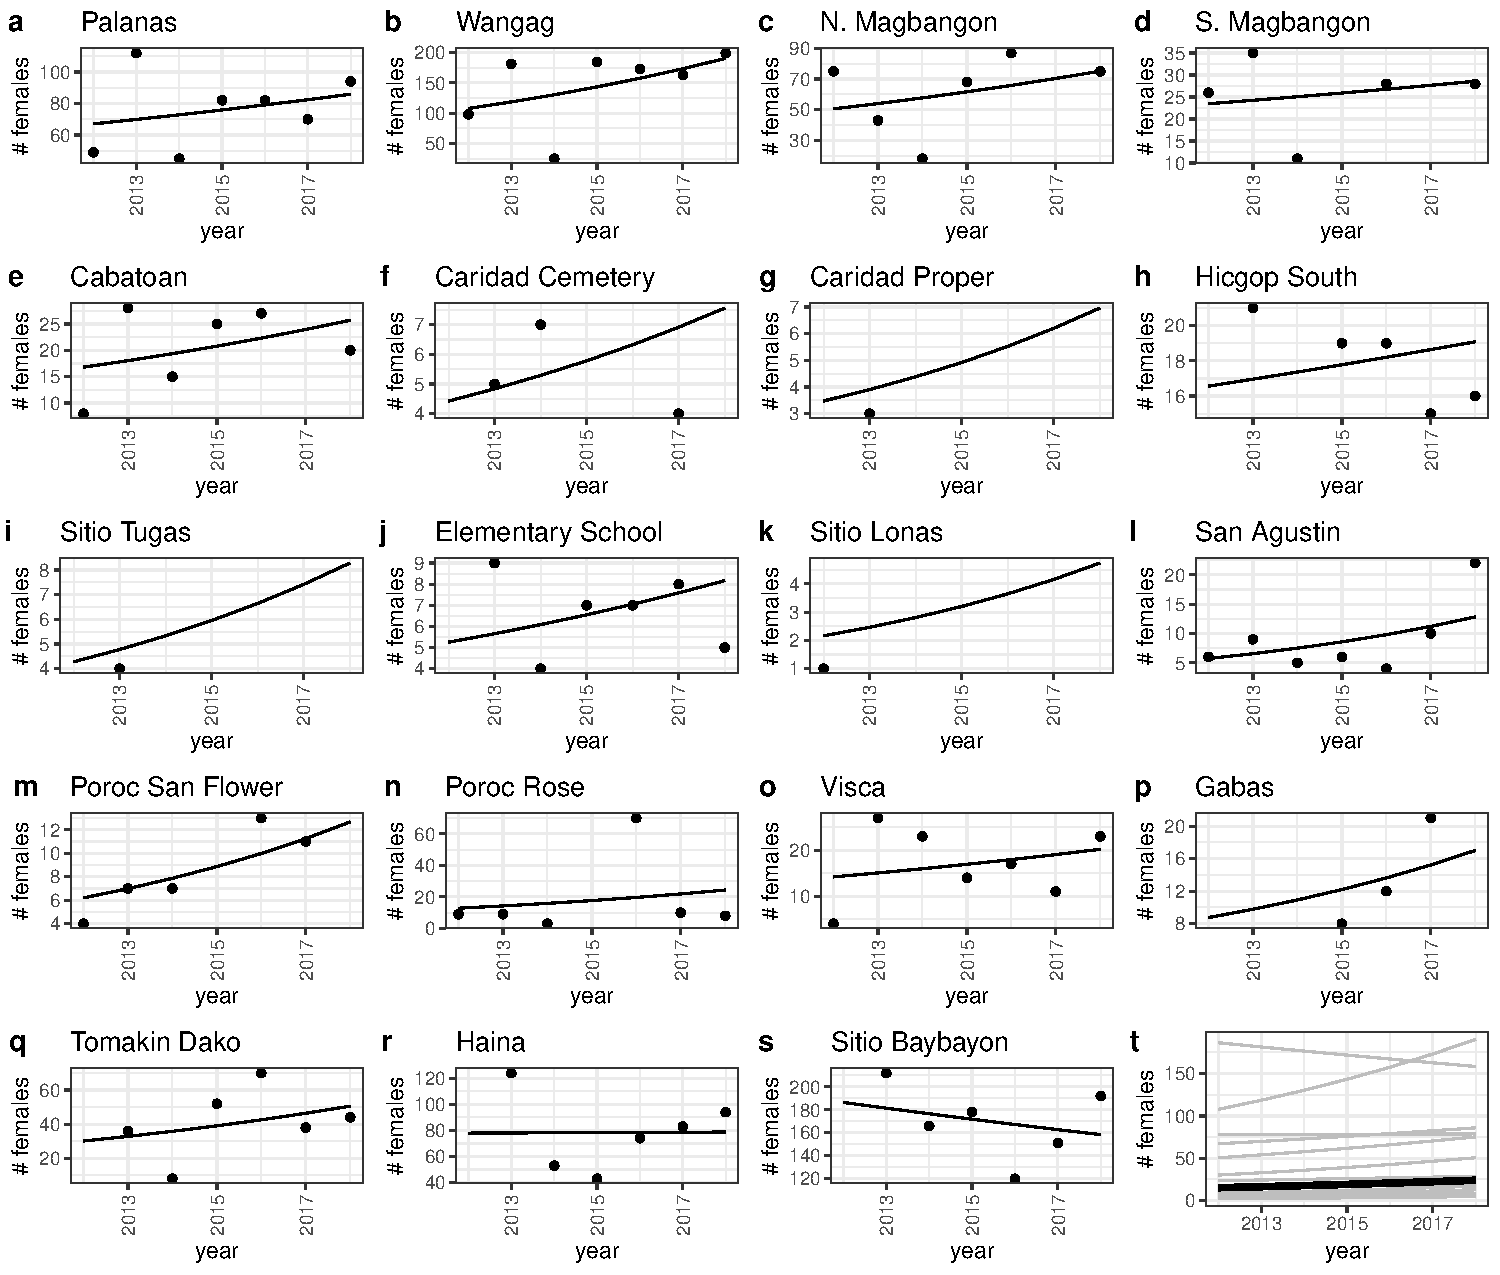
\includegraphics[width = 1.0\textwidth]{\detokenize{../Plots/FigureDrafts/Time_series_scaled_F_by_site_with_lines.pdf}}
% % 	\caption{The estimated number of females at each site over the sampling years for sites sampled in at least three years. The total number of females at each site was estimated by scaling up the number of females captured at each site in each year by the proportion of habitat sampled at that site that season (see \ref{APP_SEC_ProbHabSampled} for details) and by the average probability of capturing a fish (see \ref{APP_SEC_ProbR}). We show the estimated abundances and trend for each site individually (a-p) and a histogram of the slopes of abundance through time (q). \label{FIG_FthroughTime}}
% % \end{figure}

% From the mark-recapture analysis of tagged and genotyped fish, we estimate mean values of $L_\infty = 10.71 \text{cm}$ (range of estimates 10.50 - 10.90 cm) and $K = 0.864$ (range of estimates 0.785 - 0.944) for the von Bertalanffy growth curve parameters (eqn.\ \ref{EQN_VBL}, Fig.\ \ref{FIG_ParameterInputs}b, Table \ref{APP_TAB_Params}). For juvenile and adult (post-recruitment) survival on a log-odds scale, the best-fit model has an effect of size, with coefficient $b_a = 0.169 \pm 0.028$ SE and intercept $b_\phi = -1.83 \pm 0.231$ SE (eqn.\ \ref{EQN_Survival}). The accompanying best-fit model for log-odds recapture probability has a negative size effect and a negative effect of diver distance from the anemone (eqn.\ \ref{APP_EQN_MARKRecapture}, Fig.\ \ref{APP_FIG_RecapSizeDistEffect}).

% \begin{equation}
% \log(\frac{\phi}{1-\phi}) = b_\phi + b_a\text{size}. \label{EQN_Survival}
% \end{equation}

% Using our best estimates for growth, survival, and fecundity, we calculate a value for LEP of 1061, ranging from 39 to 10345 when we consider uncertainty in the inputs (Fig.\ \ref{FIG_Abun_LEP_LRP_LocalReplacement}b). Adult survival has the most effect on the value of LEP (Fig.\ \ref{APP_FIG_Uncertainty_LEP}), with higher values of LEP the higher annual survival of adults. 

% We estimate egg-recruit survival $S_e$ to be 7.8e-04, ranging from 1.2e-04 to 0.033 when we include uncertainty in the number of offspring assigned to parents and the probability of catching a fish (APPENDIX FIG!). When we compensate for density-dependence in our data, we estimate $S_e$ to be 0.0013, ranging from 2.1e-04 to 0.057. These are somewhat high values of egg-recruit survival compared to what we see elsewhere in the literature \citep[e.g.][]{rumrill_natural_1990, metaxas_quantifying_2009} \citep[though not unreasonable, e.g.][]{white2014planktonic, johnson2018integrating} because we scale up by the amount of habitat in our sampling area and count mortality due to dispersal to non-habitat in the dispersal probability, rather than in $S_e$. Uncertainty in the size of transition to breeding female $L_f$ has the largest effect on egg-recruit survival (Fig.\ \ref{APP_FIG_Uncertainty_RperE}); we only consider reproduction from females, to avoid double-counting, so the larger the transition size to female, the fewer tagged eggs we estimate were produced by genotyped parents and the higher egg-recruit survival. % REPHRASE THIS BETTER! THEN TALK ABOUT LRP - what that means for persistence potential.

% We estimate lifetime recruit production (LRP), the product of LEP and $S_e$, to be 0.83, with a range of 0.28 - 3.89 when we consider uncertainty in inputs. When we compensate for density-dependence, we estimate a value of 1.42 for LRP, with a range of 0.48 - 6.66. The value when we compensate for density-dependence and the range of uncertainty for both are above the threshold of one necessary for replacement before considering dispersal. This mean that individuals at our sites produce enough surviving offspring before considering dispersal to be able to replace themselves, but LRP does not tell us whether those offspring will settle within our sample sites and drive persistence. %This suggests that even without considering connectivity, the individuals at our sample populations do not produce enough offspring that survive to recruitment to replace themselves. When we consider uncertainty in our parameter estimates, we do see a few cases where LRP $>$ 1, but the majority are well below the threshold for replacement.

% We also estimate replacement for recruits from our sites returning to our sites,  $\text{LRP}_\text{local}$, which implicitly includes dispersal mortality, to be 0.09 (ranging from 0.03 to 0.44 when we include uncertainty) or 0.16 (0.05 to 0.76) when we compensate for density-dependence. With a value well below one, this suggests individuals at our sites do not replace themselves with recruits that settle in our sites, suggesting our sites do not persist as an independent network. When we calculate $\text{LRP}_\text{local}$ using all arriving recruits to our sites, however, rather than just those originating there, the best estimates are $> 1$ whether or not we compensate for density dependence (2.06, 1.22, respectively), suggesting that there is recruit-recruit replacement at our sites when we include immigrant recruits.

% We do not find any sites with SP $>$ 1, whether we compensate for density-dependence or not (Fig.\ \ref{FIG_SP_NP_realizedCmat}a), indicating that no site could persist in isolation. Given that our best estimate of LRP does not suggest replacement and only a fraction of those offspring stay at the natal site, this makes sense. We see the highest values of self-persistence at Haina ($\text{SP} = 0.079$, $0.13$ when compensating for density-dependence) and Wangag ($\text{SP} = 0.048$, $0.082$ when compensating for density-dependence), our two widest sites. 

% For network persistence, our best estimate of the dominant eigenvalue of the realized connectivity matrix $\lambda_c$ is 0.21 with a range of 0.07 - 0.92 (Fig.\ \ref{FIG_SP_NP_realizedCmat}), or 0.36 with a range 0.12 - 1.58 when we compensate for density-dependence (Fig.\ \ref{FIG_SP_NP_realizedCmat}). Our sites are likely not network persistent, as our best estimates and most of the values we see in our runs with uncertainty are below one, but network persistence is possible, as our range of estimates does exceed one when we compensate for density-dependence. We see that most of the connectivity occurs among the sites in the northern part of our sample area, from Palanas to Caridad Cemetery, and at the southern part of our sample area from Tomakin Dako to Sitio Baybayon (Fig.\ \ref{FIG_SP_NP_realizedCmat}b, d), where the largest sites are. 

% Based on our estimates of LRP, $\text{LRP}_\text{local}$, SP, and NP, it is possible but not likely that our set of sites is able to persist in isolation as a closed system. With our site configuration and dispersal kernel estimate, we would need a value of LRP of 3.99 (an egg-recruit survival of 0.0038 with our estimated value of LEP or a value of LEP of 5095 or 2975 with our estimated egg-recruit survival compensating and not compensating for density-dependence, respectively), to have a best estimate of $\lambda_c = 1$ and network persistence. 

\section*{Discussion}
In this first assessment of demographic persistence of a coastal marine metapopulation, we did not find strong evidence for either self-persistence of an individual patch or network persistence of the entire system as an isolated region. Self-persistence of one of the larger sites or network persistence of the group of sites is possible at the upper end of our estimates with uncertainty, but neither is suggested by our best estimates or 87.5\% of the estimate range. This inability to persist as an isolated region does not necessarily mean that the populations at our sites are declining, however. Our assessments of population trends - both abundance over time and replacement of recruits when we include immigrants - find that the population levels at our sites are stable or increasing slightly. Taken together, our metrics suggest that the sites in our region have stable populations on average but require input of immigrants to persist. The portion of coastline we sampled is likely a sink region of a larger metapopulation, given that there does not seem to be a long-term deline in the population. %We do not see strong evidence for the persistence of our sites as an isolated region. 

% Alternate text for paragrpah 1

% We do not see strong evidence for the persistence of our sites as an isolated region but find that they are relatively stable through time with immigration, suggesting they are a sink region within a larger metapopulation. We come to this conclusion by comparing metrics that assess persistence at three levels: 1) stability of abundance through time, 2) ability to persist as an isolated region at low abundance, and 3) ability to persist as an isolated region at current abundance levels. The positive abundance trend of an average site in our sampling region and the replacement of recruits when we include immigrant offspring suggest this region is persistent at the level of stable abundance. Our estimates of network persistence, self persistence, and local replacement with compensation for density dependence in early life indicate that our region is unlikely to be able to persist in isolation at low abundance. The estimates of those three metrics without density dependence compensation suggests that the region is also unable to persist locally at current abundance levels. Taken together as a spectrum, we suggest that this region cannot persist in isolation but receives enough input from outside areas to sustain a stable population.

% population abundance stability.  has a positive with without considering the origin in reOur estimates of network persistence, self-persistence, and local replacement suggest that local persistence of our group of sites is unlikely but within the range of possibility at the upper end of our estimates with uncertainty. When we compensate for density-dependence at early life stages, these three metrics tell us about persistence at low abundance. Without that density-dependence compensation, they tell us about our sites' ability to persist as a group at current abundance levels. Our 

% Though we do not think our sites are likely to persist Our estimates of abundance of through time at the sites 

% We find that though our sites have relatively stable abundances through time, they are not likely to be able to persist as an isolated region at either low abundances or their current population levels either at their current population levels or 

% . We see the possibility of self-persistence at two of the largest sites, Wangag and Haina, or network persistence at the upper end of our range of estimates with uncertainty, but local persistence of our region is not suggested by most of the range or our best estimates. Our estimates at abundance through time The abundances through time at our sites show a slight positive trend, suggesting that the population at our sites is not declining but relies on input of recruits from outside sites to persist. The ability of our sites to persist with immigration is confirmed by our estimate of local replacement using all arriving recruits, which is greater than one and suggests that recruits are replaced, just not by recruits of local origin. The portion of coastline we sampled is likely a sink portion of a larger metapopulation. 

% Continuum of persistence - what our different metrics mean (this is split between paragraph 1 right now and the one on density-dependence, could get pulled together?)

% What-ifs? What would our values need to be for our sites to persist? How do those/our values compare to those in the literature? THIS PARAGRAPH NEEDS HELP TO FLOW BETTER!!!
For our sites to be able to persist as a network on their own, either the number of surviving recruits produced by an average recruit (LRP) would need to be higher or more recruits would need to be retained within the region. To see a best estimate of network persistence with our existing site configuration and estimated connectivity, LRP would to be about three times higher than our best estimate, which is within our range of uncertainty (top 6.9\% of estimates) and similar to estimates of lifetime reproductive success that include dispersal to the natal reef in \textit{A. percula} in Kimbe Bay \citep{salles2020strong}, suggesting it is not an unreasonable level of production. Alternately, higher connectivity and retention of offspring among our sites could lead to network persistence. Though lack of sufficient connectivity and retention is thought to inhibit network persistence in other systems \citep[e.g., a collection of reserves for eastern oysters (\textit{Crassostrea virginica}) in the Pamlico Sound in North Carolina;][]{puckett2016metapopulation}, low production of surviving recruits due to poor habitat quality seems the more likely explanation in our system. Our dispersal kernel is comparable to those estimated for other species of reef fish, both similar in shape \citep[e.g.,][]{harrison2012larval, daloia2015patterns} and with a mean dispersal distance of a similar range to that estimated for \textit{A. percula} in Kimbe Bay \citep[13.3 and 18.9 km compared to our estimate of 8.2 km;][]{almany2017larval}, which has been found to be persistent without input from outside reefs \citep{salles_coral_2015}. Our sites have generally low reef health, however, due to anthropogenic effects such as pollution and silt from a nearby gravel mine, which affect habitat and reduce prodcution \citep[as in other clownfish systems;][]{salles2020strong, hayashi2019low}. Adult survival was lower at the two sites just downstream of the gravel mine (N.\ and S.\ Magbangon in Fig.\ \ref{APP_FIG_SurvBySizeAndSite}). %Habitat structure and quality affects prodution in other clownfish systemseffects on production have been seen both in other clownfish systems \citep[e.g.,][]{salles2020strong}, including effects of low habitat quality, e.g.,][]{hayashi2019low}. 

% Additionally, our sites are in an area that was hit in 2013 by Typhoon Haiyan, one of the strongest typhoons ever to make landfall, which destroyed much of the reef habitat in one of our northern sampling sites. This recent disturbance and generally low habitat quality could contribute to low production of surviving recruits in our sites \citep[seen in other populations with low habitat quality, e.g.,][]{hayashi2019low} necessitating subsidization by outside populations.  Lack of sufficient connectivity and retention was thought to inhibit network persistence for a collection of reserves for eastern oysters (\textit{Crassostrea virginica}) in the Pamlico Sound in North Carolina, despite demographic rates high for the species within the reserves \citep{puckett2016metapopulation}. % Even without low habitat quality, a metapopulation model of the damselfish \textit{Stegastes partitus}, also a reef fish with sedentary adults and dispersing larvae, in the Flordia Keys found that on average demographics had a stronger effect on whether a patch was a sink or a source within a metapopulation than its connectedness to other patches. RELATE TO DISPERSAL/RETENTION OF OTHER SPECIES - IS THIS POSSIBLE? HOW DO OTHER DISPERSAL KERNELS COMPARE TO OURS? MAYBE PRESENT BOTH OPTIONS, THEN MAKE SOME SORT OF COMMENT ABOUT WHICH WE THINK IS MOST LIKELY IN THIS SYSTEM? REWORK THIS PARAGRAPH ONCE HAVE THE CONTEXT NUMBERS - READS LIKE TOO MUCH ON HABITAT DISTURBANCE RIGHT NOW!

% % What-ifs? What would our values need to be for our sites to persist? How do those/our values compare to those in the literature?
% For our sites to be able to persist as a network on their own, either the number of surviving recruits produced by an average recruit (LRP) would need to be higher or more recruits would need to be retained within the region. With our existing site configuration and estimated connectivity, LRP would need to be at least 3.99 to see a best estimate of network persistence among our sites, which is within our range of uncertainty (top XX \%) but about 3-5 times higher than our best estimate. RELATE TO LITERATURE! HOW REASONABLE ARE THESE VALUES FOR A REEF FISH? Reproduction and survival at our sites might be lower than they could be due to generally low reef health and habitat quality in our sites from anthropogenic effects such as pollution and silt from a nearby gravel mine and habitat disturbance from storms. Our sites are in an area that was hit in 2013 by Typhoon Haiyan, one of the strongest typhoons ever to make landfall, which destroyed much of the reef habitat in one of our northern sampling sites. This recent disturbance and generally low habitat quality could contribute to low production of surviving recruits in our sites \citep[seen in other populations with low habitat quality, e.g.][]{hayashi2019low} necessitating subsidization by outside populations. Alternately, higher connectivity and retention of offspring among our sites could lead to network persistence. Lack of sufficient connectivity and retention was thought to inhibit network persistence for a collection of reserves for eastern oysters (\textit{Crassostrea virginica}) in the Pamlico Sound in North Carolina, depsite demographic rates high for the species within the reserves \citep{puckett2016metapopulation}. % Even without low habitat quality, a metapopulation model of the damselfish \textit{Stegastes partitus}, also a reef fish with sedentary adults and dispersing larvae, in the Flordia Keys found that on average demographics had a stronger effect on whether a patch was a sink or a source within a metapopulation than its connectedness to other patches. RELATE TO DISPERSAL/RETENTION OF OTHER SPECIES - IS THIS POSSIBLE? HOW DO OTHER DISPERSAL KERNELS COMPARE TO OURS? MAYBE PRESENT BOTH OPTIONS, THEN MAKE SOME SORT OF COMMENT ABOUT WHICH WE THINK IS MOST LIKELY IN THIS SYSTEM? REWORK THIS PARAGRAPH ONCE HAVE THE CONTEXT NUMBERS - READS LIKE TOO MUCH ON HABITAT DISTURBANCE RIGHT NOW!

% Context for LRP:
% \begin{itemize}
% 	\item Could likely calculate LRP from \cite{figueira2008small} and \cite{figueira2009connectivity}
% 	\item Check papers in \cite{burgess2014beyond}!
% \end{itemize}

% Context for dispersal kernel:
% \begin{itemize}
% 	\item previous research suggests 10km dispersal kernel spread for yellowtail clownfish \citep{pinsky2010using}
% 	\item \cite{hameed2016inverse}: \textit{Petrolisthes cinctipes}, porcelin crab, in N CA had mean dispersal distance of 6.9km (+-sd of 25km) despite 4-6 week PLD
%	\item \cite{figueira2009connectivity} has connectivity matricies and compare to others, could compare
% \end{itemize}

% For our sites to be able to persist as a network on their own, the number of surviving recruits produced by an average recruit - LRP - would likely need to be higher. With our estimated connectivity, LRP would need to be at least 3.99 to see network persistence among our sites, which is within the top of our range of uncertainty but about 3-5 times higher than our best estimates, without and with density-dependence compensation. Our best estimate of LRP when we compensate for density-dependence is greater than one, so higher connectivity and retention of offspring among our sites could lead to network persistence, but almost all surviving offspring would need to be retained. At our best estimate without density-dependence compensation, however, LRP is less than one - the average recruit only produces 0.83 of a surviving recruit of the same stage - so no amount of increased retention or connectivity, even retaining all of the recruits produced from our sites, would lead to network persistence.
 % Similarly, if other surrounding patch populations had a similar LRP, increasing the area of the network to include them would also not achieve network persistence. If nearby sites have higher egg production or survival to recruit, however, it might not take much of an increase in area considered to create a persistence network. Nearby reef sites such as Cuatro Islas have higher quality habitat and could be contributing recruits to our sites. ADD THIS BIT TO PARAGRAPH BELOW OR SEPARATE ONE

% % reconcile with dispersal distance, spatial what-ifs - paragraph edited with Malin's edits
% We do not find clear evidence for network persistence for our sites despite estimates of the mean dispersal distance of \textit{A. clarkii} from previous genetic work \citep[11 km,][]{pinsky2010using} and from our samples \citep{catalanoInPrepconnectivity} that are well within the 30 km span of our sites. Though the length of our sampling region is more than twice the mean dispersal distance, usually sufficient for persistence of a population in an isolated reserve \citep[e.g.][]{lockwood2002effects}, our sampling region contains only about 20\% habitat, rather than a continuous stretch. For a habitat configuration more like our system, habitat patches (reserves) spaced on a coastline with non-habitat in between, theory suggests that peristence requires about 40\% of the coastline to be preserved or a minimum patch size of 1.25 times the mean dispersal distance \citep{lockwood2002effects}. Our largest site, Haina, is only about 0.8km wide, about 10 (CHECK!) times less than the mean dispersal distance, so it is possible we do not have enough habitat in our region for network persistence. Additionally, the configuration our sites is such that the four largest sites are at the edge of our sampling region and send half of their recruits away from our sites. Our sensitivity test to proportion habitat suggests that about 2.75 times more habitat in our sampling region would give a best estimate with network persistence and a width of XX for the site with the highest adult survival would give self persistence. 

% reconcile with dispersal distance, spatial what-ifs - paragraph edited with Will's edits after Malin's edits
We do not find clear evidence for network persistence for our sites despite estimates of the mean dispersal distance of \textit{A. clarkii} from previous genetic work \citep[11 km,][]{pinsky2010using} and from our samples \citep[8.2 km,][]{catalanoInPrepconnectivity} that are well within the 30 km span of our sites. Though the length of our sampling region is more than twice the mean dispersal distance, usually sufficient for persistence of a population in an isolated reserve \citep[e.g.][]{lockwood2002effects}, our sampling region contains only about 20\% habitat, rather than a continuous stretch, which may be too low of habitat coverage to support network persistence. Our sensitivity test to proportion habitat suggests that about 2.75 times more habitat in our sampling region would give a best estimate with network persistence, with 50\% of our estimates showing persistence ($\lambda_{C_{DD}} \geq 1$) at about 30\% habitat. Our individual sites are likely too small to see self-persistence: the largest site, Haina, is only about 0.8km wide, about 10 times smaller than the mean dispersal distance. This is in contrast to the findings on reefs surrounding the isolated Kimbe Island, where the overall population of \textit{A. percula} and several lagoon subpopulations of similar size as our sites were self-persistent \citep{salles_coral_2015}. Our sites are in an area that was hit in 2013 by Typhoon Haiyan, one of the strongest typhoons ever to make landfall, so reef habitat has recently been destroyed in the area, including one of our northern sampling sites. The suggestion of a habitat shortage in our sampling region is partially dependent on our assumption that larvae land in non-habitat between patches and die. Larvae have some navigational and habitat-finding capabilities \citep[e.g.][]{elliott1995host, fisher2005swimming}, so we could be underestimating their ability to find habitat in our calculations, which would decrease the amount of habitat required for network persistence. % In our site with the highest LEP, a width of XX would be required for self-persistence. 

We suggest that our region is a sink area of a larger metapopulation but the area required for the larger persistent metapopulation depends on the production and connectivity of outside patches. If surrounding patch populations have a similar LRP and level of connectivity as our sites, increasing the area of the network to include them also would not achieve network persistence. If nearby sites have higher egg production or egg-recruit survival, however, it might not take much of an increase in area considered to create a persistent network. Nearby reef sites such as Cuatro Islas, with higher coral cover and less silt, could have higher survival of fish and be contributing recruits to our sites. % COULD CONSIDER ADDING BIT ABOUT POLLUTION HERE INSTEAD OF IN LRP PARAGRAPH ABOVE. ANYTHING WE CAN SAY ABOUT THE SCALE OF OTHER METAPOPS AS A COMPARISON?

An alternative to our sampled sites as a sink portion of a larger metapopulation is that variability in demography or dispersal on a longer scale than our sampling time could lead to persistence. For example, rockfish on the west coast of the United States have highly variable and episodic recruitment, where successful recruitment events occur on the decadal scale and sustain the population until the next strong recruitment event \citep[e.g.,][]{tolimieri2005roles}. Though perhaps not as extreme as in the California Current system, ocean connectivity is still variable in the Coral Triangle region surrouding our study sites, with estimates suggesting that 20 year simulations are necessary to capture the full extent \citep{thompson2018variability}. Our study, though relatively long term, could have missed a particularly strong recruitment event that would enable local persistence of the set of populations we sampled. 
% %%% FIGURE OUT WHERE TO PUT THIS IDEA OF LONGER-TERM PATTERNS OF VARIABILITY IN DEMOGRAPHY AS AN ALTERNATIVE TO A SINK!
% An alternative is that there are longer-term patterns of variability in the demography (perhaps in larval production or survival) that lead to persistence…perhaps there is a once-in-10-years sweepstakes success that then sustains the population for many years. Even this fairly long-term study may have missed such an event. (this may not be the spot in the paper to raise this possibility…maybe later)

% find sufficient for persistence of an isolated reserve, their estimate assumes continuous habitat within the reserve and our region is only about 20\% habitat. For a habitat configuration more similar to our system, habitat patches (reserves) spaced on a coastline with non-habitat in between, they find that either 40\% of the coastline needs to be preserved or a minimum patch size must be 1.25 times the mean dispersal distance to ensure persistence. Our largest site, Haina, is only about 0.8 km wide, about 10 times less than the mean dispersal distance, so it is possible we do not have enough habitat in our region for network persistence, exacerbated by our 4 largest sites being at the edges of our area and sending half of their recruits away from our sites. Our low, and possibly below-replacement, estimate for LRP also suggests that lack of persistence in these sites is not due to excessive dispersal out of the area but due to low production and survival of offspring. The reef health and habitat quality in our sites is generally low, due anthropogenic effects such as pollution and silt from a nearby gravel mine, and habitat disturbance due to storms. Our sites are in an area that was hit in 2013 by Typhoon Haiyan, one of the strongest typhoons ever to make landfall, which destroyed much of the reef habitat in some of our northern sampling areas. This recent disturbance and generally low habitat quality could contribute to low production of surviving recruits in our sites \citep[seen in other populations with low habitat quality, e.g.][]{hayashi2019low} necessitating subsidization by outside populations.

Though we estimate abundance trends and do not find overall declines, it is possible we could have missed declines due to our sampling design. Our sampling study was designed for mark-recapture analyses rather than a comprehensive habitat or abundance estimate so we did not sample all areas of all sites each year. We scale up the number of fish we caught to account for those we missed using the proportion of metal-tagged anemones we visited, which assumes that all tagged anemones are equally likely to be sampled. In reality, tags that no longer have anemones next to them are likely harder to find and sample. If anemones are disappearing over time at our sites, we might be overestimating the number of fish present and missing that our site are declining and not persistent even with outside input.

% uncertainty
NEED TO EDIT THIS UNCERTAINTY PARAGRAPH!
% Outline for uncertainty paragraph:
% 1: why is accounting for uncertainty important
% 2: what did we find 
% 3: compare to other sensitivity/elasticity assessments other people did 
Including uncertainty in our empirical estimates of demographic and dispersal parameters allows us to better understand how likely it is that the population is persistent and which processes contribute the most uncertainty. We see a wide range of estimated metric values, spanning of network persistence for our set of sites to far from it. In our study, demographic parameters, particularly adult survival, also have a large effect on whether or not we think the population is persistent. Other metapopulation studies also find higher sensitivity to demographic rather than connectivity parameters \citep[e.g., on source or sink status in bicolor damselfish;][]{figueira2009connectivity}, including particular sensitivity to adult survival \citep[on metapopulation growth rate in mussels;][]{carson2011evaluating}. Our estimates of connectivity are simpler than our estimates of demography, with no spatial variability \citep[which can be important in understanding demographic connectivity;][]{johnson2018integrating}, and a more thorough assessment could alter their relative effect on persistence, but this suggests that sufficient offspring production and survival has a larger effect on persistence at these relatively small scales of connectivity. Uncertainty in our sampling, particularly how likely we are to capture a fish, however, contributes the most uncertainty to whether we determine the population to be persistent, highlighting the challenge of estimating these metrics empirically. For a marine metapopulation, our system is relatively uncomplicated; as we accumulate more empirical assessments of metapopulations to compare to our expectations from theory and models, we will have to think carefully about how to handle uncertainty as we move to tackling larger and more complicated systems.

% Accounting for uncertainty in our field estimates of demographic processes and dispersal allows us to better understand how likely it is that the population is persistent within the range of our estimated parameters. We see a wide range of metric values, depending on the particular inputs we use  

% By including uncertainty in our estimates of demographic and dispersal parameters, we get a clearer picture of how likely persistence is at our sites and which processes contribute the most uncertainty. TAKE A BIT OF PARAGRAPH BELOW? THEN TALK ABOUT THOSE OTHER PAPERS

% We see considerable uncertainty in our estimate of persistence metrics depending on the particular input values we use (Figs.\ \ref{FIG_Abun_LEP_LRP_LocalReplacement}, \ref{APP_FIG_Uncertainty_NP}). Our highest estimate for LRP is about 24 times more than our lowest estimate and our highest NP estimate is about 22 larger than our lowest, spanning the range between network persistence for our set of sites to far from it. Measuring demographic and dispersal parameters in the field is challenging; in the face of limited and imperfect data, characterizing uncertainty and propagating it from our estimates of demographic and dispersal inputs through to our estimates of persistence metrics is important to contextualize our results. In our study, uncertainty in egg-recruit survival \citep[a commonly challenging parameter to estimate, e.g.][]{johnson2018integrating,hameed2016inverse}, partially driven by uncertainty in how likely we are to capture recruits during sampling (Fig.\ \ref{APP_FIG_Uncertainty_RperE}), has a large effect on whether or not we think our populations are persistent. For a marine metapopulation, our system is relatively uncomplicated and yet still hard in which to concretely assertain persistence. As we accumulate more empirical assessments of metapopulations to compare to our expectations from theory and models, we will have to think carefully about how to handle uncertainty as we move to tackling larger and more complicated systems. %Examples of when the empirical result doesn't match the model expectation?

% Caveats - density-dependence, could also discuss site-specific demographic parameters?
Persistence criteria, such as those detailed in \cite{hastings_persistence_2006} and \cite{burgess2014beyond}, ask whether a population at low abundance can grow and recover rather than going extinct. Density-dependence is often ignored at low abundances \citep{botsford2019population} so is not explicitly considered in persistence metrics. In real populations, however, it can be challenging to estimate density-independent demographic rates, as density-dependence is occurring in the population as it is sampled. In \textit{A. clarkii}, density-dependence is likely most important immediately post-settlement, as for many fish species, but is also relatively easy to measure at that point and accounted for in our analyses. Density-dependence could continue to be important throughout the life history, however, due to the social hierarchies in colonies of clownfish \citep[e.g.][]{buston2011determinants}. In other species of clownfish, individuals on the same anemone maintain strict size spacing, restricting their food intake and growth to avoid encroaching on the position of another fish and being attacked or evicted \citep[seen in \textit{A. percula},][]{buston2003forcible, buston2003social}. This suggests that while fish are in the pre-reproductive queue, density-dependence may lower growth rates compared to the growth of fish alone on an anemone, as would be the case in a population at low abundance. We include the primary effect of density-dependence on our estimate of egg-recruit survival but other estimates, particularly growth and survival, would also likely be higher in the absence of density-dependence and increase LRP.

% Either as part of the paragraph above or as a new paragraph, talk about how our findings that abundance is stable through time is somewhat dependent on the anemone habitat available being constant (which it might not be in recent years). We can find empty tags, so scaling by proportion tags sampled should give us the right estimate, but in reality tags without anemones are harder to find (and maintain) so unsampled tags are probably more likely to not have anemones (or clownfish on the anemones) than sampled tags. Talk about habitat degredation noticed in most recent field season, what relaxing this assumption might mean for our results.

% Comment from Will - talk about LRP_local difference from lambda somewhere! "You don’t really mention LRP-local here, but it would be good someplace in the ms to talk about how LRP-local and lambda differ as persistence metrics. LRP-local is basically assuming that the entire metapopulation is a single well-mixed unit, while the lambda value is accounting for the spatial structure and multi-generation dynamics."

% Paragraph 6: Wrap-up - NEED TO RE_WRITE THIS IN LIGHT OF NEW RESULTS!! Malin suggested cutting entirely because pretty repetitive of what came before...
% Our estimates of persistence metrics suggest that it is possible but not likely that the region of sites we sample persist as a network without outside input, despite covering an area more than twice the estimated mean dispersal distance for our focal species. Our estimate of LRP near the threshold of one required for replacement (slightly $ < 1$ when we do not correct for density-dependence, slightly $ > 1$ when we do), suggests that dispersal is not likely the primary reason our sites do not persist as a network. If density-dependence is strongly present in our data such that our corrected estimate is the best, then our sites could persist if there were no losses to dispersal. Otherwise, our sites do not produce enough offspring for replacement regardless of dispersal patterns, possibly due to worsening habitat quality. This is a reminder that dispersal is only part of the persistence story for metapopulations; even areas that seem large enough to contain a persistent network based on dispersal distance will not be able to persist in isolation if they have low production and survival of offspring. We do find recruits coming back to our region, and even to their natal site, but broader connectivity to more productive sites likely enables our sites to persist.

Understanding persistence is critical for management of spatial-structured populations, such as siting marine protected areas XX, assessing habitat fragmentation risks, and conserving species in the face of climate change XX. Though models and theory provide us with expectations, we are only recently beginning to be able to tackle these questions of persistence empirically in model systems such as clownfish and other sedentary tropical reef fish \citep[e.g.,][]{salles_coral_2015, johnson2018integrating}. With parentage analyses now being extended to temperate species \citep[e.g.,][]{baetscher2019dispersal} and better understanding of how biophysical models compare to larval dispersal patterns \citep{bode2019validation} we are beginning to move beyond model species and investigate persistence in harvested and spatially-managed systems \citep[e.g.,][]{garavelli2018population}. Our study shows the importance of long term sampling and careful consideration of the different demographic processes that affect our metric calculations, such as density-dependence and sampling biases, to understand marine population dynamics in empirical systems.

% %%% TO ADD TO DISCUSSION !
% These are somewhat high values of egg-recruit survival compared to what we see elsewhere in the literature \citep[e.g.][]{rumrill_natural_1990, metaxas_quantifying_2009} \citep[though not unreasonable, e.g.][]{white2014planktonic, johnson2018integrating} because we scale up by the amount of habitat in our sampling area and count mortality due to dispersal to non-habitat in the dispersal probability, rather than in $S_e$. 

% % What did we learn about metapopulation theory? Think about both marine and non-marine systems here
% % Papers to discuss: Johnson et al. 2018, Salles et al. 2015, 

% %%% NEED A GOOD CONCLUDING PARAGRAPH!
% Note from Will - also, he is happy to take a crack at writing it: "I think we need a short but strong closing paragraph here that reminds us why it is important to know about persistence (spatial management! conservation in the face of climate change! etc). Remind us that for a long time we did not have a way to tackle this problem but are beginning to do it using model systems like clownfish. Same types of parentage analysis are now being extended to temperate species (e.g. Baetscher et al; I will send you a copy) so we are beginning to extend beyond clownfish. This work shows the importance of long term study and of thinking carefully about the implications of different demographic processes that influence calculations (e.g, DD, recruit sampling biases) in order to understand marine population dynamics."


% % DISCUSSION IN PREVIOUS DRAFT

% We do not see strong evidence for persistence in our metric estimates. We see no evidence for self-persistence where an individual site could persist alone and weak evidence for network persistence; it is possible at the upper end of our range of estimates with uncertainty but not suggested by most of the range or our best estimates (Fig.\ \ref{FIG_SP_NP_realizedCmat}). The abundances through time at our sites do not show a clear directional change, however, suggesting that the population at our sites is relatively constant but relies on input of recruits from outside sites to persist. The portion of coastline we sampled is likely a sink portion of a larger metapopulation. 

% For our sites to be able to persist as a network on their own, the number of surviving recruits produced by an average recruit - LRP - would likely need to be higher. With our estimated connectivity, LRP would need to be at least 3.99 to see network persistence among our sites, which is within the top of our range of uncertainty but about 3-5 times higher than our best estimates, without and with density-dependence compensation. Our best estimate of LRP when we compensate for density-dependence is greater than one, so higher connectivity and retention of offspring among our sites could lead to network persistence, but almost all surviving offspring would need to be retained. At our best estimate without density-dependence compensation, however, LRP is less than one - the average recruit only produces 0.83 of a surviving recruit of the same stage - so no amount of increased retention or connectivity, even retaining all of the recruits produced from our sites, would lead to network persistence. Similarly, if other surrounding patch populations had a similar LRP, increasing the area of the network to include them would also not achieve network persistence. If nearby sites have higher egg production or survival to recruit, however, it might not take much of an increase in area considered to create a persistence network. Nearby reef sites such as Cuatro Islas have higher quality habitat and could be contributing recruits to our sites.   

% % reconcile with dispersal distance
% We do not find clear evidence for network persistence for our sites despite estimates of the mean dispersal distance of \textit{A. clarkii} from previous genetic work \citep[11 km,][]{pinsky2010using} and from our samples \citep[8.25 km, with 95\% confidence interval 7.41 to 9.36,][]{catalanoInPrepconnectivity} that are well within the 30 km span of our sites. Though the width of our sampling region is more than twice the mean dispersal distance, which \cite{lockwood2002effects} find sufficient for persistence of an isolated reserve, their estimate assumes continuous habitat within the reserve and our region is only about 20\% habitat. For a habitat configuration more similar to our system, habitat patches (reserves) spaced on a coastline with non-habitat in between, they find that either 40\% of the coastline needs to be preserved or a minimum patch size must be 1.25 times the mean dispersal distance to ensure persistence. Our largest site, Haina, is only about 0.8 km wide, about 10 times less than the mean dispersal distance, so it is possible we do not have enough habitat in our region for network persistence, exacerbated by our 4 largest sites being at the edges of our area and sending half of their recruits away from our sites. Our low, and possibly below-replacement, estimate for LRP also suggests that lack of persistence in these sites is not due to excessive dispersal out of the area but due to low production and survival of offspring. The reef health and habitat quality in our sites is generally low, due anthropogenic effects such as pollution and silt from a nearby gravel mine, and habitat disturbance due to storms. Our sites are in an area that was hit in 2013 by Typhoon Haiyan, one of the strongest typhoons ever to make landfall, which destroyed much of the reef habitat in some of our northern sampling areas. This recent disturbance and generally low habitat quality could contribute to low production of surviving recruits in our sites \citep[seen in other populations with low habitat quality, e.g.][]{hayashi2019low} necessitating subsidization by outside populations.

% % uncertainty
% We see considerable uncertainty in our estimate of persistence metrics depending on the particular input values we use (Figs.\ \ref{FIG_Abun_LEP_LRP_LocalReplacement}, \ref{APP_FIG_Uncertainty_NP}). Our highest estimate for LRP is about 24 times more than our lowest estimate and our highest NP estimate is about 22 larger than our lowest, spanning the range between network persistence for our set of sites to far from it. Measuring demographic and dispersal parameters in the field is challenging; in the face of limited and imperfect data, characterizing uncertainty and propagating it from our estimates of demographic and dispersal inputs through to our estimates of persistence metrics is important to contextualize our results. In our study, uncertainty in egg-recruit survival \citep[a commonly challenging parameter to estimate, e.g.][]{johnson2018integrating,hameed2016inverse}, partially driven by uncertainty in how likely we are to capture recruits during sampling (Figs.\ \ref{APP_FIG_Uncertainty_RperE}, \ref{APP_FIG_Uncertainty_RperE_DD}), has a large effect on whether or not we think our populations are persistent. For a marine metapopulation, our system is relatively uncomplicated and yet still hard in which to concretely assertain persistence. As we accumulate more empirical assessments of metapopulations to compare to our expectations from theory and models, we will have to think carefully about how to handle uncertainty as we move to tackling larger and more complicated systems. %Examples of when the empirical result doesn't match the model expectation?

% % Caveats - density-dependence, could also discuss site-specific demographic parameters?
% Persistence criteria, such as those detailed in \cite{hastings_persistence_2006} and \cite{burgess2014beyond}, ask whether a population at low abundance can grow and recover rather than going extinct. Density-dependence is often ignored at low abundances \citep[e.g.][]{caswell_matrix_2001, hastings_simple_2006} so is not explicitly considered in persistence metrics. In real populations, however, it can be challenging to estimate density-independent demographic rates, as density-dependence is occurring in the population as it is sampled. In \textit{A. clarkii}, density-dependence is likely most important in early life stages, as for many fish species, but could play an important role throughout the life history due to the social hierarchies in colonies of clownfish \citep[e.g.][]{buston2011determinants}. In other species of clownfish, individuals on the same anemone maintain strict size spacing, restricting their food intake and growth to avoid encroaching on the position of another fish and being attacked or evicted \citep[seen in \textit{A. percula},][]{buston2003forcible, buston2003social}. This suggests that while fish are in the pre-reproductive queue, density-dependence may lower growth rates compared to the growth of fish alone on an anemone, as would be the case in a population at low abundance. We attempt to account for the primary effect of density-dependence on our estimate of egg-recruit survival but other estimates, particularly growth and survival, would also likely be higher in the absence of density-dependence and increase LRP.

% % Paragraph 6: Wrap-up
% Our estimates of persistence metrics suggest that it is possible but not likely that the region of sites we sample persist as a network without outside input, despite covering an area more than twice the estimated mean dispersal distance for our focal species. Our estimate of LRP near the threshold of one required for replacement (slightly $ < 1$ when we do not compensate for density-dependence, slightly $ > 1$ when we do), suggests that dispersal is not likely the primary reason our sites do not persist as a network. If density-dependence is strongly present in our data such that our compensated estimate is the best, then our sites could persist if there were no losses to dispersal. Otherwise, our sites do not produce enough offspring for replacement regardless of dispersal patterns, possibly due to worsening habitat quality. This is a reminder that dispersal is only part of the persistence story for metapopulations; even areas that seem large enough to contain a persistent network based on dispersal distance will not be able to persist in isolation if they have low production and survival of offspring. We do find recruits coming back to our region, and even to their natal site, but broader connectivity to more productive sites likely enables our sites to persist.


% Our estimates of survival probabilities are similar to those estimated for other species of clownfish, particulary our relationship with size where small fish have a low annual survival and the largest fish have a high annual survival (CITATIONS, Buston paper, also compare to Salles et al. 2015). Our fecundity estimates are lower than those for \textit{A. clarkii} in temperate areas, almost XX times lower (CITATIONS, Ochi papers - 17,500 eggs/yr/female, from Bell 1976).

% Density-dependence notes: Settling clownfish can be ”driven from the anemone within hours of their arrival [38,47]” - p.1884 in Buston et al. (2011), citations are Buston (2003a) and Elliott et al. (1995)

% Context for dispersal kernel:
% \begin{itemize}
% 	\item previous research suggests 10km dispersal kernel spread for yellowtail clownfish \citep{pinsky2010using}
% 	\item \cite{hameed2016inverse}: \textit{Petrolisthes cinctipes}, porcelin crab, in N CA had mean dispersal distance of 6.9km (+-sd of 25km) despite 4-6 week PLD
% \end{itemize}

% Context for larval mortality or egg-recruit mortality:
% \begin{itemize}
% 	\item check \cite{white2014planktonic}
% 	\item check estimate in \cite{johnson2018integrating}
% \end{itemize}

% Context for adult mortality
% \begin{itemize}
% 	\item \cite{salles_coral_2015}: check paper, possibly 0.18-0.49 for J, 0.09-0.44 for M, 0.19-0.55 for F (are the ranges for subpops? biannual mortality rates?), orange clownfish (\textit{Ampiphrion percula}) in Kimbe Bay
% 	\item \cite{buston2003social} (or possibly the other 2003 Buston paper...), 12.9\% mortality per year for \textit{Ampiprion percula} in Papua New Guinea
% \end{itemize}

\newpage{}

\section*{Figures}

% Figure 1 - schematic
\begin{figure}[H] % Schematic
	\centering
	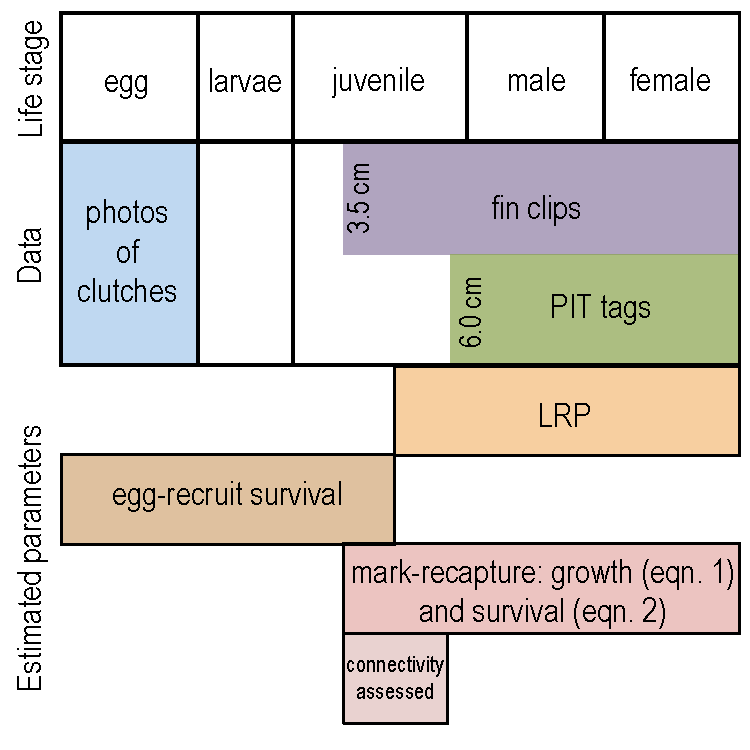
\includegraphics[width = 1.0\textwidth]{\detokenize{../Plots/Schematic/Schematic.pdf}}
	\caption{The data collected for fish at each life stage and how they match to the equations and metrics estimated. We consider recruits to be offspring in their first year of settlement, represented by the 3.5-6.0 cm range. \label{FIG_Schematic}} 
\end{figure}

% Figure 2 - map + photo
\begin{figure}[H] % Map + clownfish photo
	\centering
	\includegraphics[width = 1.0\textwidth]{\detokenize{../Plots/FigureDrafts/Map_and_photo.pdf}}
	\caption{a) Map of the sites along the coast of Leyte in the Philippines. From north to south, the patches are: 1) Palanas, 2) Wangag, 3), North Magbangon, 4) South Magbangon, 5) Cabatoan, 6) Caridad Cemetery, 7) Caridad Proper, 8) Hicgop South, 9) Sitio Tugas, 10) Elementary School, 11) Sitio Lonas, 12) San Agustin, 13) Poroc San Flower, 14) Poroc Rose, 15) Visca, 16) Gabas, 17) Tomakin Dako, 18) Haina, and 19) Sitio Baybayon. b) Zoomed-in map of the two northern-most sites, Palanas and Wangag, to show anemone arrangement with anemones colored as occupied by \textit{A.\ clarkii} (green), occupied by other clownfish species (orange), or unoccupied by clownfish (grey). c) An example anemone occupied by \textit{A.\ clarkii} in a typical habitat at the sites. The metal anemone tag is visible just above the anemone on the rock.  \label{FIG_Map_and_photo}} 
\end{figure}

% Figure 3 - demographic and dispersal inputs
\begin{figure}[H] % demographic parameters: survival curve, growth curve, dispersal kernel, transition size to female 
	\centering
	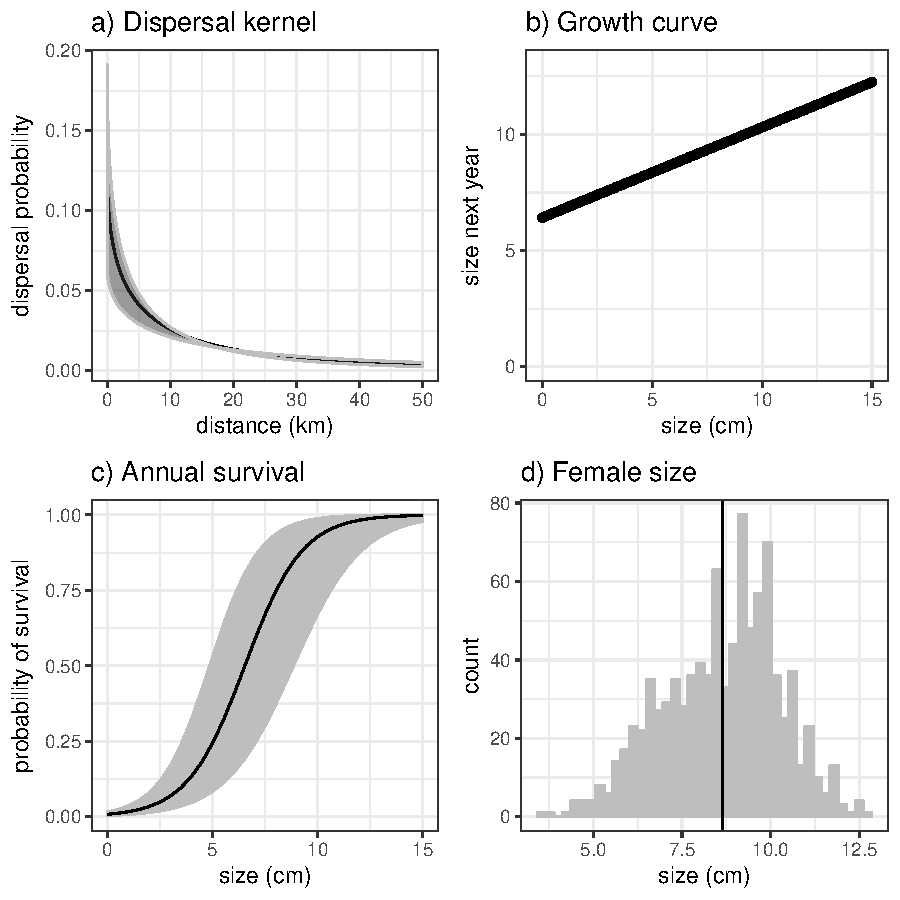
\includegraphics[width = 1.0\textwidth]{\detokenize{../Plots/FigureDrafts/Parameter_inputs.pdf}}
	\caption{Best estimates (solid black line) and uncertainty (grey) for dispersal (a), growth, including the 1:1 line in thick black (b), post-recruit annual survival at Palanas as an example site (c), and size at female transition (d) parameters. Best est  \label{FIG_ParameterInputs}}
\end{figure}

% Figure 4 - abudance trends, LEP, LRP, local replacement metrics
\begin{figure}[H] % abudance trends and LEP, LRP LRP_local shown with uncertainty, line for best estimate (using mean offspring size as recruit size)
	\centering
	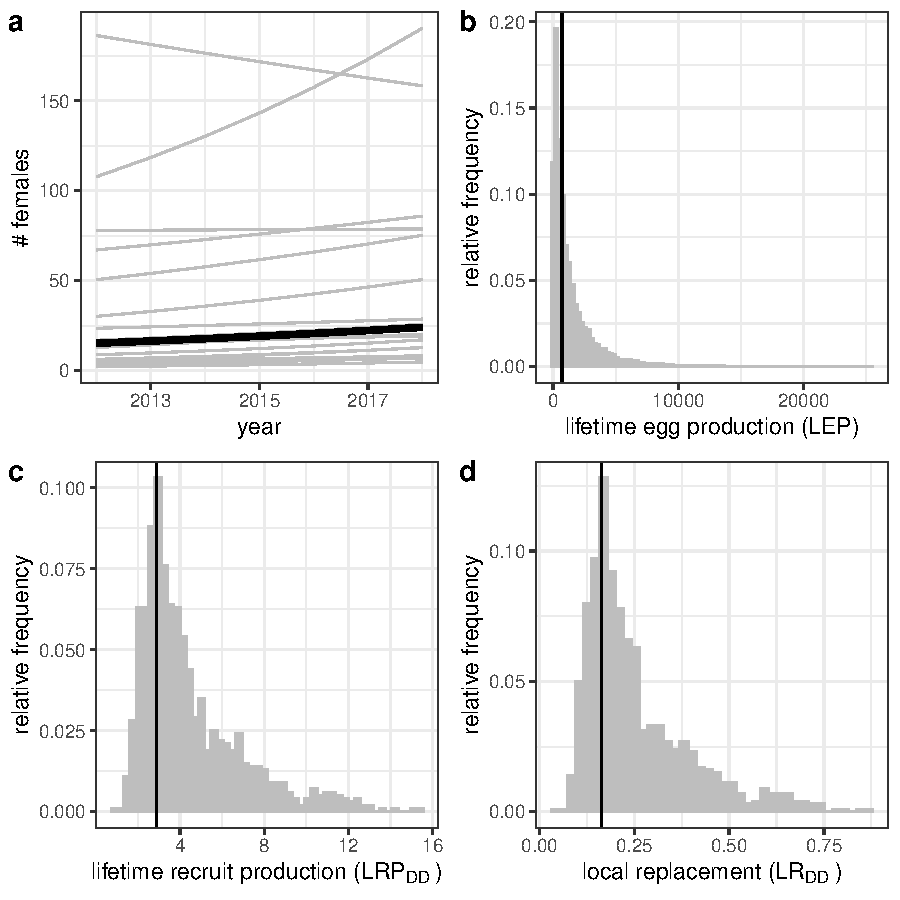
\includegraphics[width = 1.0\textwidth]{\detokenize{../Plots/FigureDrafts/Abundance_LEP_LRP_LocalReplacement_FreqPlots.pdf}}
	\caption{Estimates of a) estimated abundance of females over time at each individual site (grey lines) and for an average site (black line), b) individual-site LEP for all sites with the best estimate averaged across sites (black line), c) average $\text{LRP}_{DD}$ across sites, and d) local replacement, showing the best estimate (black solid line) and range of estimates considering uncertainty in the inputs (grey). Estimates of LRP and local replacement include compensation for density-dependent mortality in early life stages. \label{FIG_Abun_LEP_LRP_LocalReplacement}}
\end{figure}

% % Old SP figure
% \begin{figure}[H] % SP with line for best estimate (using mean offspring size as recruit size)
% 	\centering
% 	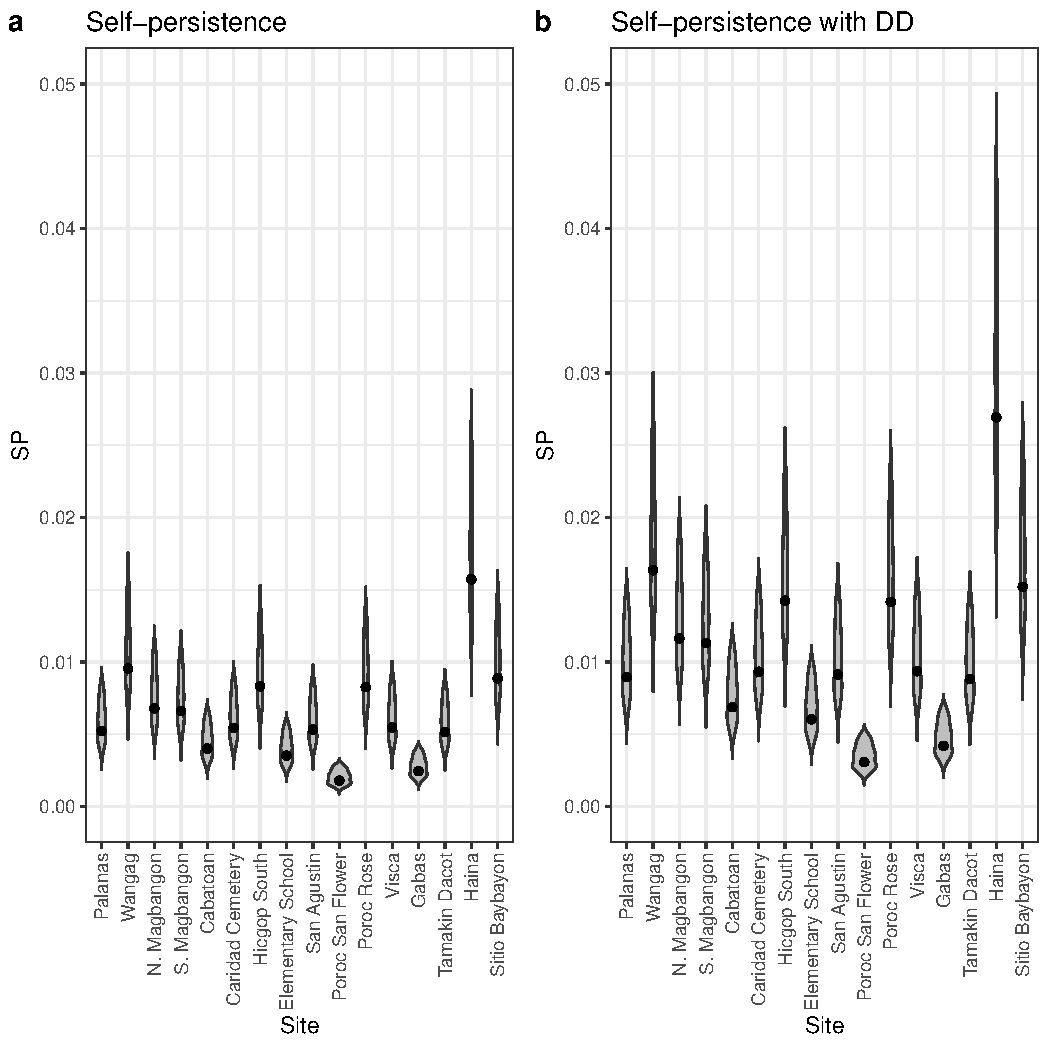
\includegraphics[width = 1.0\textwidth]{\detokenize{../Plots/FigureDrafts/SP_hists_by_site_noSLSTCP.pdf}}
% 	\caption{Values of self-persistence at each site, showing the best estimate (black point) and range of estimates considering uncertainty in the input paramters. No site reaches the value SP $\geq$ 1 necessary to be self-persistent. The estimates in (b) attempt to compensate for density-dependence in early life stages in our data, while the estimates in (a) do not. \label{FIG_SP}}
% \end{figure}

% Figure 5 - SP, realized connectivity matrix, and NP
\begin{figure}[H] % NP with line for best estimate (using mean offspring size as recruit size), realized connectivity matrix for best estimate - should re-do without Sitio Lonas, Sitio Tugas, Caridad Proper!
	\centering
	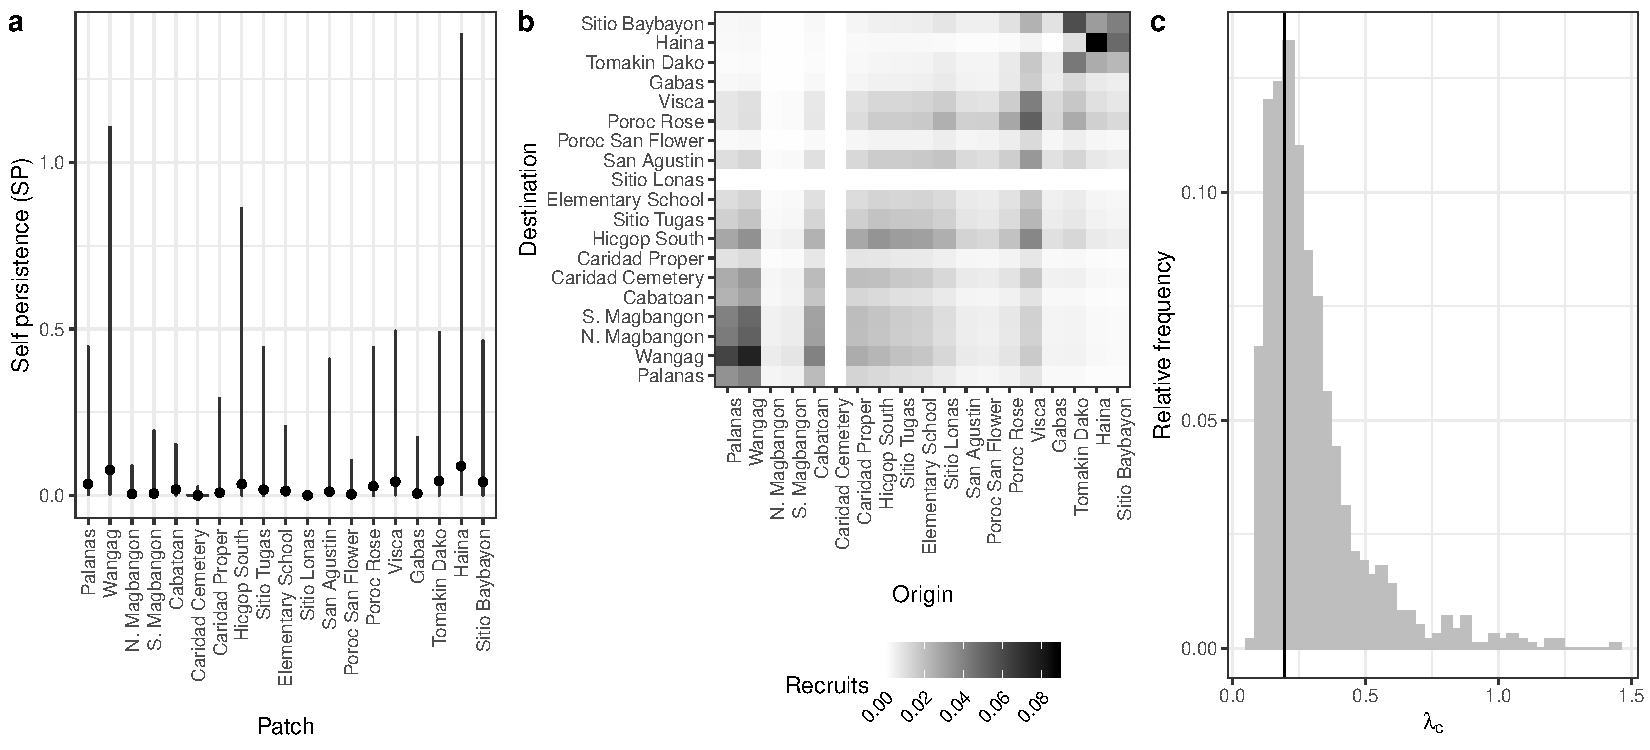
\includegraphics[width = 1.0\textwidth]{\detokenize{../Plots/FigureDrafts/SP_NP_connMatrixR_freq.pdf}}
	\caption{Values of self-persistence (a), realized connectivity among sites (b), and network persistence (c). All estimates include compensation for density-dependence in early life stages. For self-persistence (a) and network persistence (c), the best estimate is shown with in black (point for (a), line for (c)) and the range of estimates considering uncertainty is shown in grey. \label{FIG_SP_NP_realizedCmat}}
\end{figure}

% Figure 6 - what-if, changing proportion habitat sampled
\begin{figure}[H] 
	\centering
	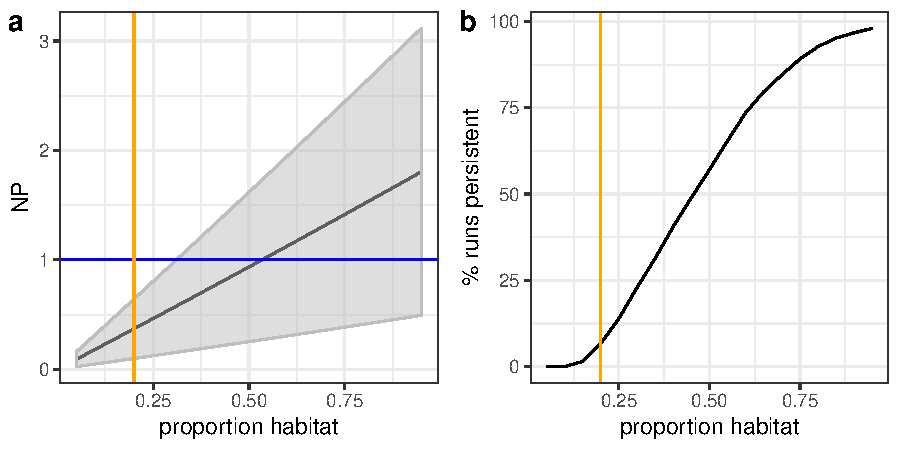
\includegraphics[width = 1.0\textwidth]{\detokenize{../Plots/FigureDrafts/NP_perc_hab_perc_persist_sd_ribbon.pdf}}
	\caption{Sensitivity of network persistence to the proportion of the sampling region that is habitat. (a) The best estimate of $\lambda_{c_{DD}}$ with the standard deviation of the estimates with uncertainty for 19 patches of equal size and spacing with adult survivals for an average patch. (b) The percentage of estimates from the runs in (a) with $\lambda_{c_{DD}} \geq 1$ with increasing proportion habitat. \label{FIG_WI_PERC_HAB}}
\end{figure}
\newpage{}

{\LARGE Appendix}

\appendix

\renewcommand{\theequation}{A\arabic{equation}}
% redefine the command that creates the equation number.
\renewcommand{\thetable}{A\arabic{table}}
\setcounter{equation}{0}  % reset counter 
\setcounter{figure}{0}
\setcounter{table}{0}
\numberwithin{equation}{section}
\numberwithin{figure}{section}

\section{Summary of parameters} %% HAVEN'T UPDATED THIS WITH NEW VALUES YET!!

%[\textit{Need to clarify somewhere what kind of distributions are going into the uncertainty runs (drawn from data, uniform across a range, 95\% confidence bounds, etc.)}]
% Make table prettier
\begin{centering}
\begin{longtable}{|p{1.1in}|p{1.2in}|p{1.2in}|p{1in}|p{1.5in}|}
\hline 
\textbf{Parameter} & \textbf{Description} & \textbf{Best estimate} & \textbf{Range in uncertainty runs} & \textbf{Notes} \\ \hline
$k_d$ & scale parameter in dispersal kernel & -2.33 & -2.81 to -1.22 & eqn.\ \ref{EQN_integratingDK}, estimated using methods in \cite{bode2018estimating} in Catalano et al.\ (in prep) \\ \hline
$\theta$ & shape parameter in dispersal kernel & 1.19 & 0.63 to 2.04 & eqn.\ \ref{EQN_integratingDK}, estimated using methods in \cite{bode2018estimating} in Catalano et al.\ (in prep) \\ \hline
$L_\infty$ & average asymptotic size (cm) in von Bertalanffy growth curve & 10.70 cm & 9.81 to 11.65 cm & eqn.\ \ref{EQN_VBL} \\ \hline
$K$ & growth coefficient in von Bertalanffy growth curve &  0.864 & 0.80 to 0.91 & eqn.\ \ref{EQN_VBL} \\ \hline  
$b_{\phi_{Cabatoan}}$ & intercept for adult survival at 0 cm at Cabatoan & -1.78 & $\pm$ 0.33 standard error & on a log-odds scale, eqn.\ \ref{APP_EQN_Survival} \\ \hline 
$i_{\phi_{Cardidad Cemetery}}$ & addition to intercept for survival at Caridad Cemetery & -19.61 & $\pm$ 2994 standard error & on a log-odds scale, eqn.\ \ref{APP_EQN_Survival} \\ \hline
$i_{\phi_{Elementary School}}$ & addition to intercept for survival at Elementary School & -0.11 & $\pm$ 0.41 standard error & on a log-odds scale, eqn.\ \ref{APP_EQN_Survival} \\ \hline
$i_{\phi_{Gabas}}$ & addition to intercept for survival at Gabas & -0.42 & $\pm$ 0.58 standard error & on a log-odds scale, eqn.\ \ref{APP_EQN_Survival} \\ \hline
$i_{\phi_{Haina}}$ & addition to intercept for survival at Haina & 0.12 & $\pm$ 0.35 standard error & on a log-odds scale, eqn.\ \ref{APP_EQN_Survival} \\ \hline
$i_{\phi_{Hicgop South}}$ & addition to intercept for survival at Hicgop South & -0.06 & $\pm$ 0.46 standard error & on a log-odds scale, eqn.\ \ref{APP_EQN_Survival} \\ \hline
$i_{\phi_{N. Magbangon}}$ & addition to intercept for survival at N. Magbangon & -1.31 & $\pm$ 0.38 standard error & on a log-odds scale, eqn.\ \ref{APP_EQN_Survival} \\ \hline
$i_{\phi_{Palanas}}$ & addition to intercept for survival at Palanas & 0.24 & $\pm$ 0.26 standard error & on a log-odds scale, eqn.\ \ref{APP_EQN_Survival} \\ \hline
$i_{\phi_{Poroc Rose}}$ & addition to intercept for survival at Poroc Rose & -0.19 & $\pm$ 0.44 standard error & on a log-odds scale, eqn.\ \ref{APP_EQN_Survival} \\ \hline
$i_{\phi_{Poroc San Flower}}$ & addition to intercept for survival at Poroc San Flower & -0.52 & $\pm$ 0.48 standard error & on a log-odds scale, eqn.\ \ref{APP_EQN_Survival} \\ \hline
$i_{\phi_{San Agustin}}$ & addition to intercept for survival at San Agustin & -0.47 & $\pm$ 0.50 standard error & on a log-odds scale, eqn.\ \ref{APP_EQN_Survival} \\ \hline
$i_{\phi_{Sitio Baybayon}}$ & addition to intercept for survival at Sitio Baybayon & 0.02 & $\pm$ 0.26 standard error & on a log-odds scale, eqn.\ \ref{APP_EQN_Survival} \\ \hline
$i_{\phi_{S. Magbangon}}$ & addition to intercept for survival at S. Magbangon & -1.08 & $\pm$ 0.48 standard error & on a log-odds scale, eqn.\ \ref{APP_EQN_Survival} \\ \hline
$i_{\phi_{Tomakin Dako}}$ & addition to intercept for survival at Tomakin Dako & 0.39 & $\pm$ 0.33 standard error & on a log-odds scale, eqn.\ \ref{APP_EQN_Survival} \\ \hline
$i_{\phi_{Visca}}$ & addition to intercept for survival at Visca & 0.33 & $\pm$ 0.35 standard error & on a log-odds scale, eqn.\ \ref{APP_EQN_Survival} \\ \hline
$i_{\phi_{Wangag}}$ & addition to intercept for survival at Wangag & 0.35 & $\pm$ 0.25 standard error & on a log-odds scale, eqn.\ \ref{APP_EQN_Survival} \\ \hline
$b_a$ & size effect for adult survival & 0.15 & $\pm$ 0.03 standard error & on a log-odds scale, eqn.\ \ref{APP_EQN_Survival} \\ \hline
%$b_{p_r}$ & intercept for recapture probability from mark-recapture analysis & 2.10 & $\pm$ 0.849 standard error & on a log-odds scale, not used in persistence estimates \\ \hline
%$b_1$ & size effect for recapture & -0.161 & $\pm$ 0.088 standard error & on a log-odds scale, not used in persistence estimates \\ \hline
%$b_2$ & distance effect for recapture & -0.196 & $\pm$ 0.023 standard error & on a log-odds scale, not used in persistence estimates \\ \hline
$\beta_e$ & coefficient for eyed eggs & -0.608 & & eqn.\ \ref{EQN_Fec}, Yawdoszyn et al.\ (in prep) \\ \hline
$\beta_l$ & size effect in eggs-per-clutch relationship & 2.39 & & eqn.\ \ref{EQN_Fec}, Yawdoszyn et al.\ (in prep) \\ \hline
$b$ & intercept in eggs-per-clutch relationship at female size 0 cm & 1.17 & & eqn.\ \ref{EQN_Fec}, Yawdoszyn et al.\ (in prep) \\ \hline
$c_e$ & egg clutches per year & 11.9 & & eqn.\ \ref{EQN_Fec}, \cite{holtswarth2017fecundity} \\ \hline
$\text{size}_\text{recruit}$ & size (cm) of recruited offspring & mean of size of offspring in parentage analysis = 4.37 cm & 3.5 - 6.0 cm & drawn from uniform distribution across range \\ \hline
$\text{size}_{\text{recruit}, sd}$ & standard deviation of size of a recruit & 0.1 & & used in discretization of IPM for LEP \\ \hline
$\text{size}_{sd}$ & standard deviation distribution of sizes of a fish in the next year & 1.45 & & used in discretization of IPM for LEP, estimated from range of sizes for fish starting at 7.4-7.6 cm and recaptured a year later \\ \hline
$L_s$ & minimum size in LEP IPM & 0 cm & & eqn.\ \ref{EQN_LEP} \\ \hline
$U_s$ & maximum size in LEP IPM & 15 cm & & eqn.\ \ref{EQN_LEP} \\ \hline
%$S_e$ & egg-recruit survival & & &  \\ \hline
%$E_c$ & eggs per clutch & depends on female size (eqn.\ \ref{EQN_Fec}) & & relationship from Yawdoszyn et al.\ (in prep) \\ \hline
$L_f$ & size at transition to female & 9.32 cm & 5.2 - 12.7 cm & drawn from distribution in data \\ \hline
$R_m$ & number of offspring matched to parents & 62	offspring & & eqn.\ \ref{EQN_EggRecruitSurv} \\ \hline
$N_g$ & number of genotyped parents & 1719 fish & & eqn.\ \ref{EQN_EggRecruitSurv} \\ \hline
$P_h$ & proportion of sites sampled cumulatively across time & 0.41 & & eqn.\ \ref{EQN_EggRecruitSurv}, details in \ref{APP_SEC_ProbHabSampled} \\ \hline
$P_d$ & proportion of dispersal kernel area from each site covered by our sampling region & 0.28 & & eqn.\ \ref{EQN_EggRecruitSurv}, details in \ref{APP_SEC_PropDispKernelSampled} \\ \hline 
$P_c$ & probability of capturing a fish & 0.56 & drawn from beta distribution with parameters $\alpha_{P_c} = 1.44$ and $\beta_{P_c} = 1.13$ & eqn.\ \ref{EQN_EggRecruitSurv}, details in \ref{APP_SEC_ProbR} \\ \hline
$P_s$ & proportion of our sampling region that is habitat & 0.20 & & eqn.\ \ref{EQN_EggRecruitSurv}, details in \ref{APP_SEC_PropHabInSampledRegion} \\ \hline
$\text{DD}$ & proportion of habitat that would be available without density-dependence at settlement & 1.71 & & eqn.\ \ref{EQN_EggRecruitSurv} \\ \hline
$p_U$ & proportion of anemones unoccupied by clownfish & 0.53 & & used to estimate DD \\ \hline
$p_A$ & proportion of anemones occupied by \textit{A. clarkii} & 0.38 & & used to estimate DD \\ \hline
\caption{Summary of parameter symbols, definitions, and values.}\label{APP_TAB_Params} 
\end{longtable}
\end{centering}

\section{Method details}

\subsection{Proportion of habitat sampled} \label{APP_SEC_ProbHabSampled}

We used tagged anemones to estimate the proportion of habitat sampled at each site in each year ($P_{h_{i,t}}$). We tagged each anemone that is home to \textit{A. clarkii}, with a metal tag, which is relatively permanent and easy to re-sight (the anemone tag is visible above the anemone in Fig.\ \ref{FIG_Map_and_photo}c), so we consider the total number of metal tags at each site to be the total number of anemones that are habitat. We divide the number of tagged anemones visited each sampling year by the total number of metal tags at that site to get the proportion of habitat sampled. We use proportion of anemones rather than proportion of total site area because anemones, and therefore habitat quality, are unevenly distributed across the site; areas we did not visit are likely to have a lower density of anemones than the areas we did sample.

For scaling the number of tagged recruited offspring to account for areas of our sites we did not sample, we use the overall proportion habitat sampled across all sites and sampling years ($P_h$). We sum the metal-tagged anemones we visited across all sites and years to get the total number of metal-tagged anemones we visited while sampling. We then divide that by the number of anemones we could have sampled, the sum of total metal-tagged anemones across all sites multiplied by the number of sampling years, to get the overall proportion habitat sampled across our sites and sampling years.

%\textit{Add details about how sometimes it is >1 if the site doesn't have metal tags? Mention plastic tags?}

\begin{table}
\begin{centering}
\begin{tabular}{|l|r|r|r|r|r|r|r|r|}
\hline 
\multicolumn{2}{|c|}{} & \multicolumn{7}{|c|}{\% Habitat surveyed} \\ \hline
Site & \# Total anems & 2012 & 2013 & 2014 & 2015 & 2016 & 2017 & 2018 \\ \hline
Cabatoan & 26 & 42 & 58 & 58 & 65 & 73 & 0 & 62 \\ \hline
Caridad Cemetery & 4 & 0 & 75 & 50 & 0 & 50 & 50 & 50 \\ \hline
Elementary School & 8 & 0 & 100 & 38 & 88 & 88 & 88 & 100 \\ \hline
Gabas & 9 & 0 & 0 & 0 & 44 & 44 & 67 & 0 \\ \hline
Haina & 104 & 0 & 6 & 13 & 13 & 10 & 56 & 80 \\ \hline
Hicgop South & 18 & 0 & 67 & 22 & 28 & 56 & 83 & 78 \\ \hline
N. Magbangon & 105 & 5 & 12 & 40 & 63 & 63 & 0 & 5 \\ \hline
S. Magbangon & 34 & 41 & 56 & 32 & 0 & 65 & 0 & 71 \\ \hline
Palanas & 137 & 29 & 58 & 47 & 63 & 85 & 86 & 86 \\ \hline
Poroc Rose & 13 & 100 & 100 & 69 & 31 & 23 & 69 & 69 \\ \hline
Poroc San Flower & 11 & 100 & 82 & 73 & 73 & 55 & 82 & 64 \\ \hline
San Agustin & 17 & 94 & 65 & 71 & 65 & 100 & 82 & 76 \\ \hline
Sitio Baybaon & 260 & 0 & 14 & 30 & 33 & 30 & 41 & 80 \\ \hline
Tomakin Dako & 50 & 0 & 24 & 22 & 36 & 34 & 60 & 68 \\ \hline
Visca & 13 & 100 & 100 & 23 & 38 & 62 & 85 & 62 \\ \hline
Wangag & 296 & 18 & 32 & 42 & 34 & 26 & 49 & 68 \\ \hline
\end{tabular}
\end{centering}
\caption{Table showing the percent of metal-tagged anemones surveyed at each site in each sampling year.}\label{APP_TAB_PercHabSampled}
\end{table}

\newpage{}

\subsection{Probability of capturing a fish, from recapture dives} \label{APP_SEC_ProbR}

We use mark-recapture data from recapture dives done within a sampling season to estimate the probability of capturing a fish. During some of the sampling years, portions of the sites were sampled again within a few weeks of the original sampling dives. We assume there is no mortality of tagged fish between the original sampling dives and the recapture dives because they are so close in time and that fish do not change their behavior or reponse to divers, so therefore assume that the probability of recapturing a fish is the same as the probablity of capturing a fish on a sampling dive. For each recapture dive, we use GPS tracks of the divers to identify the anemones covered in the recapture dive and the set of PIT-tagged fish encountered on those anemones during the original sampling dives. We estimate the probability of capture $P_c$ as the number of tagged fish caught during the capture dive $m_2$ divided by the total number of fish caught on the recapture dive $n_2$: $P_c = \frac{m_2}{n_2}$. The value of $P_c$ from each recapture dive is reported in Table \ref{APP_TAB_RecapDives}.

We use the mean $P_c$ across all 14 recapture dives, covering XX sites in 3 sampling seasons (2016, 2017, 2018), as our best estimate. Because there are so few recapture dives compared to the number of times we calculate the metrics to show the range of uncertainty, we represent the probability of capture as a distribution, rather than sampling directly from the values calculated for each recapture dive. The distribution of capture probabilities across the 14 dives is quite skewed so we represent it as a beta distribution, using the mean $\mu_{P_c}$ and variance $V_{P_c}$ of the set of 14 values to find the appropriate $\alpha_{P_c}$ and $\beta_{P_c}$ parameters, where 

\begin{eqnarray}
\alpha_{P_c} &=& (\frac{1-\mu_{P_c}}{V_{P_c}} - \frac{1}{\mu_{P_c}}) \mu_{P_c}^2 \\
\beta_{P_c} &=& \alpha_{\mu_{P_c}} \times \frac{1}{\mu_{P_c} - 1}. \label{APP_EQN_ProbCapBetaDistParams}  % Should I cite a source for this?
\end{eqnarray}

% Should I include a table of the recapture probs for each recapture dive, including site and year?
The mean of the individual capture probability values is $\mu_{P_c} = 0.56$, with variance $V_{P_c} = 0.069$, which gives beta distribution parameters $\alpha_{P_c} = 1.44$ and $\beta_{P_c} = 1.13$. We sample 1000 values from the beta distribution, then truncate the sample to only values larger than the lowest value of $P_c$ estimated in an individual dive (0.20), to avoid extremely low values that are sometimes randomly sampled from the distribution but are unrealistically low. We then sample with replacement from the truncated set to get a vector of values the length of the number of runs.

\textit{Talk to Katrina to fill out table with data that went into recapture calcs}

\begin{table}
\begin{centering}
\begin{tabular}{|l|r|r|r|r|}
\hline
Site & Year & $m_2$ & $n_2$ & $P_c$ \\ \hline
& & & & 0.56 \\ \hline
& & & & 0.26 \\ \hline
& & & & 0.89 \\ \hline
& & & & 0.67 \\ \hline
& & & & 0.20 \\ \hline
& & & & 0.83 \\ \hline
& & & & 0.47 \\ \hline
& & & & 0.20 \\ \hline
& & & & 0.83 \\ \hline
& & & & 1.0 \\ \hline
& & & & 0.33 \\ \hline
& & & & 0.58 \\ \hline
& & & & 0.63 \\ \hline
& & & & 0.41 \\ \hline
\end{tabular}
\end{centering}
\caption{Table showing the site, year, number of fish caught on sample dives on the anemones resampled during the recapture dive ($m_2$), number of fish caught on the recapture dive ($n_2$) for each recapture dive.} \label{APP_TAB_RecapDives}
\end{table}

\newpage{}

\subsection{Scaling up recruits}

To estimate the total number of offspring produced by our genotyped parents that survive to recruitment, we scale up the number of matched offspring caught during sampling ($R_m$) to account for recruits we could have missed (Fig.\ \ref{APP_FIG_RecruitScalingSchematic}). We scale up by 1) the cumulative proportion of habitat we sampled at our sites over time ($P_h$) to account for recruits at anemones we did not sample (details in \ref{APP_SEC_ProbHabSampled}), 2) the probability of capturing a fish if we sampled its anemone ($P_c$) to account for fish that escaped during sampling (details in \ref{APP_SEC_ProbR}), 3) the proportion of the dispersal kernel from our sites within of our sampling region ($P_d$) to account for fish that dispersed outside of our sampling area (details in \ref{APP_SEC_PropDispKernelSampled}), and 4) the proportion habitat in our sampling region ($P_s$) to avoid counting mortality of fish dispersing to non-habitat within our region twice (in both the estimate of total recruits and in the integrated dispersal kernel) (details in \ref{APP_SEC_PropHabInSampledRegion}), and 5) the proportion of anemones occupied by \textit{A. clarkii} ($DD$) to account for density-dependent mortality of settling recruits.

\begin{figure}[H] % Scaling up recruits
	\centering
	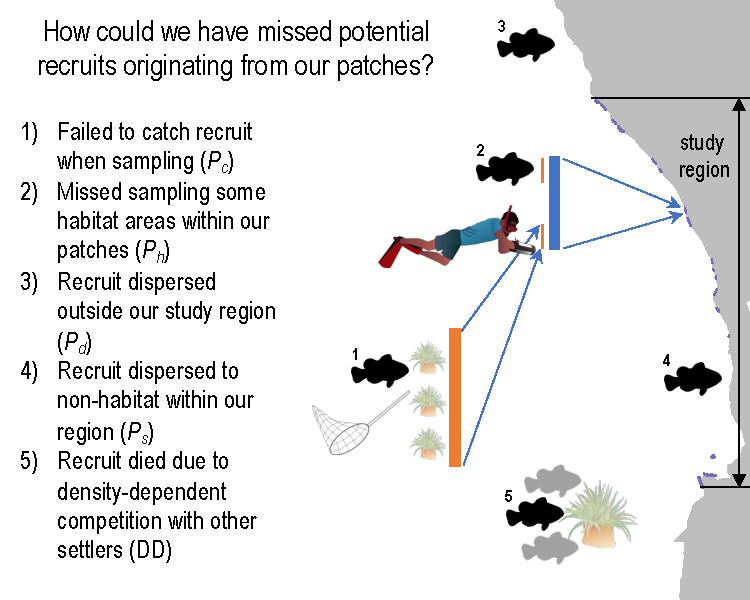
\includegraphics[width = 1.0\textwidth]{\detokenize{../Plots/UndercountingRecruits/RecruitScalingSchematic.pdf}}
	\caption{Schematic of five ways we could have missed recruits while sampling and used to scale up our raw estimate of recruits from matched offspring. \label{APP_FIG_RecruitScalingSchematic}}
\end{figure}

\newpage{}

\paragraph{Proportion of dispersal kernel area sampled} \label{APP_SEC_PropDispKernelSampled}

To account for recruits that dispersed outside our sampling region, we find the proportion of the dispersal kernels from all parents that falls within our sampling region. For each of the nineteen sites, we find the area ($A_i$) under the kernel from the center of the site to the north edge of the sampling area ($d_N$) (northern-most tagged anemone at Palanas, the northern-most site) and the center of the site to the south edge of the sampling area ($d_S$) (southern-most tagged anemone at Sitio Baybayon, the southern-most site), then multiply by the number of genotyped parents at that site ($N_{g_i}$). We add the total areas together, then divide by the sum of the total area under the dispersal kernel in both directions (1 when kernel is normalized to 0.5) multiplied by the total number of genotyped parents ($N_g$) to get the proportion of the total dispersal kernel area covered by our sampling region ($P_d$):

\begin{equation} 
%p_{A, B}(d) = \int_{d_1}^{d_2} e^k e^{-(e^k d)^\theta}  dd. \label{EQN_integratingDK}
A_i(d) = N_{g_i} \int_{0}^{d_N} z e^{-(zd)^\theta}  dd, \label{EQN_DK_area_within_sampling_region}
\end{equation}

\begin{equation}
P_d = \frac{\sum_{i=1}^{19} A_i}{N_g}.
\end{equation}

% \begin{equation}
% %p(d) = e^k e^{-(e^k d)^\theta}. \label{EQN_DispKernel}
% p(d) = ze^{-(zd)^\theta}. \label{EQN_DispKernel}
% \end{equation}

\begin{figure}[H] % Proportion of dispersal kernel area from each site sampled
	\centering
	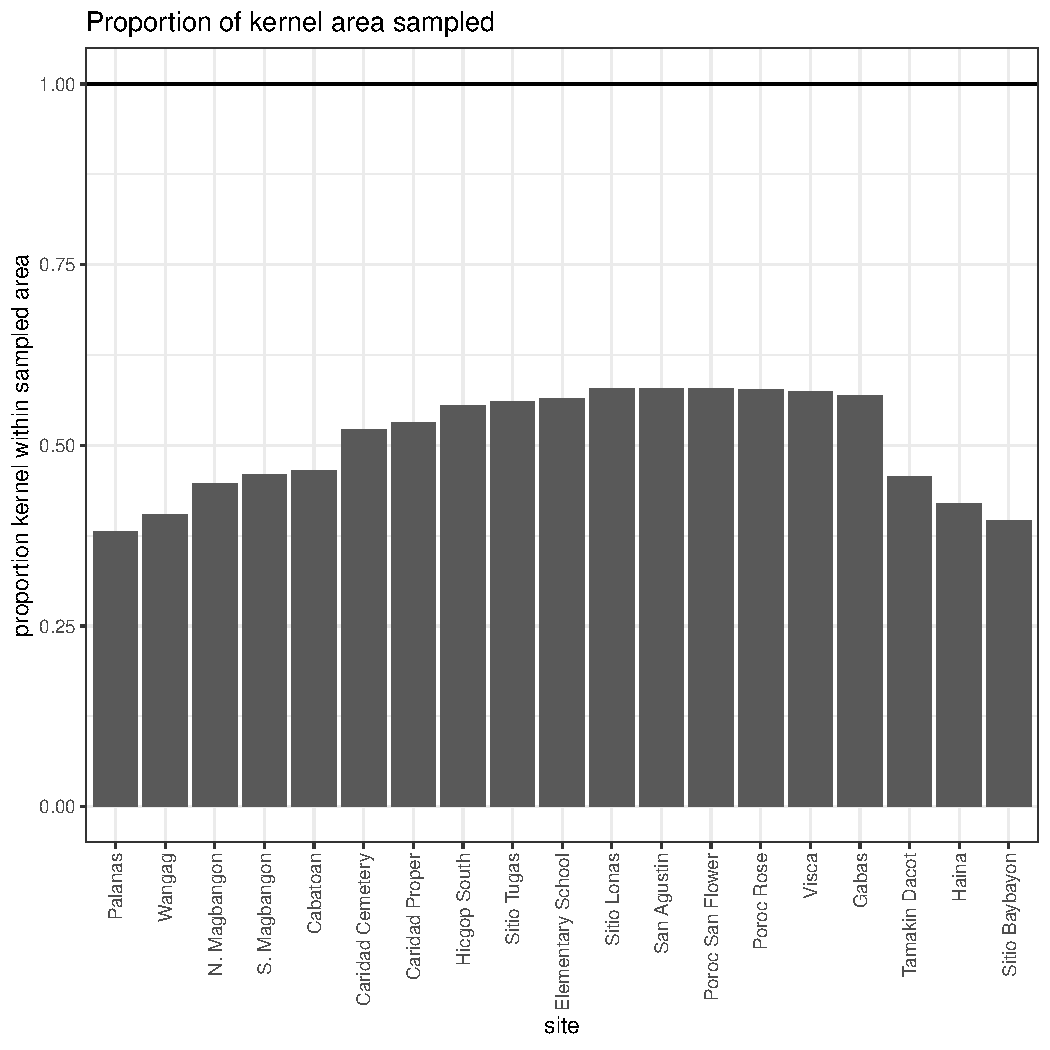
\includegraphics[width = 1.0\textwidth]{\detokenize{../Plots/FigureDrafts/Prop_of_kernel_area_sampled_by_site.pdf}}
	\caption{Proportion of the dispersal kernel area from the center of each site covered by our sampling. Our overall proportion is weighted by the number of parents at each site. \label{APP_FIG_PropDispKernelAreaSampled}}
\end{figure}

\newpage{}

\paragraph{Proportion habitat in sampling area} \label{APP_SEC_PropHabInSampledRegion}

We assume that larvae are unable to navigate to habitat if they attempt to settle on an unsuitable patch, though clownfish larvae do likely have some ability both to sense good settlement areas, either by detecting host anemones \citep{elliott1995host, arvedlund1999host} or conspecifics \citep[e.g.][for coral reef fish more broadly]{lecchini2005experimental}, and swim in particular direction \citep[e.g.][]{bellwood2001relative, fisher2005swimming}. To avoid counting mortality due to settling on non-habitat twice - once in scaling up our matched recruits, which only includes those who settled on habitat, and once in integrating the dispersal kernel, we scale our estimate of total surviving recruits from our patches by the proportion of our sampling region that is habitat ($P_s$). We find $P_s$ by summing the lengths of all of our sites, which run approximately north-south, and dividing that by the total distance north-south of our sampling region, giving $P_s = 0.20.$

%CHECK THAT CLIMATE CHANGE AND DISPERSAL FOLDER FOR CITATIONS - THAT PAPER THAT SAID OA AFFECTS REEF FISH SENSORY ABILITIES PROBABLY HAS GOOD CITATIONS. ALSO 1992 paper I just downloaded and other that is open.
\newpage{}

\subsection{Full set of MARK models} \label{APP_MARKModels}
We consider the following set of models in MARK for survival ($\phi$) and recapture ($p$) probability, including effects of size ($S$), minimum distance from diver to anemone during surveys ($D$), time ($t$), and site ($i$) (Table \ref{APP_TAB_MARKmodels}):

\begin{table}
\begin{centering}
\begin{tabular}{|p{2in}|p{2.5in}|p{0.75in}|p{0.75in}|}
\hline 
\textbf{Model} & \textbf{Model description} & \textbf{AICc} & \textbf{dAICc} \\ \hline
$\phi \sim S$, $p \sim S+D$ & survival size, recapture size+distance & 3348.861 & 0 \\ \hline
$\phi \sim S$, $p \sim D$ & survival size, recapture distance & 3359.998 & -11.1371 \\ \hline
$\phi$, $p \sim D$ & survival constant, recapture distance & 3383.175 & 34.3141 \\ \hline
$\phi$, $p \sim S+D$ & survival constant, recapture size+distance & 3384.959 & 36.0981 \\ \hline
$\phi \sim t$, $p$ & survival time, recapture constant & 3408.342 & 59.4816 \\ \hline
$\phi \sim i$, $p$ & survival site, recapture constant & 3440.842 & 91.98112 \\ \hline
$\phi \sim i$, $p \sim S+D$ & survival site, recapture size+distance & 3440.842 & 91.98112 \\ \hline
$\phi$, $p \sim t$ & survival constant, recapture time & 3453.609 & 104.74839 \\ \hline
$\phi \sim S$, $p \sim S$ & survival size, recapture size & 3527.710 & 178.84940 \\ \hline
$\phi$, $p$ & survival constant, recapture constant & 3570.908 & 222.04690 \\ \hline
\end{tabular}
\end{centering}
\caption{}\label{APP_TAB_MARKmodels}
\end{table}


% From the mark-recapture analysis of tagged and genotyped fish, we estimate mean values of $L_\infty = 10.71 \text{cm}$ (range of estimates 10.50 - 10.90 cm) and $K = 0.864$ (range of estimates 0.785 - 0.944) for the von Bertalanffy growth curve parameters (eqn.\ \ref{EQN_VBL}, Fig.\ \ref{FIG_ParameterInputs}b, Table \ref{APP_TAB_Params}). For juvenile and adult (post-recruitment) survival on a log-odds scale, the best-fit model has an effect of size, with coefficient $b_a = 0.169 \pm 0.028$ SE and intercept $b_\phi = -1.83 \pm 0.231$ SE (eqn.\ \ref{EQN_Survival}). The accompanying best-fit model for log-odds recapture probability has a negative size effect and a negative effect of diver distance from the anemone (eqn.\ \ref{APP_EQN_MARKRecapture}, Fig.\ \ref{APP_FIG_RecapSizeDistEffect}).

The best model for post-recruitment annual survival $\phi$ has a positive size effect ($b_a = 0.169 \pm 0.028$ SE UPDATE THESE NUMBERS!) with intercepts varying by site (eqn.\ \ref{APP_EQN_Survival}, Fig.\ \ref{APP_FIG_SurvBySizeAndSite}). The best model for recapture probability $p_r$ has a negative effect of size ($b_1 = -1.816 \pm 0.080$ SE UPDATE THESE NUMBERS!) and a negative effect of diver distance from anemone ($b_2 = -0.171 \pm 0.021$ SE UPDATE THESE NUMBERS!), with intercept $b_{p_r} = 17.93 \pm 0.858$ SE UPDATE THESE NUMBERS! (eqn.\ \ref{APP_EQN_MARK_Recapture}, Fig.\ \ref{APP_FIG_RecapSizeDistEffect}), suggesting divers are less likely to recapture larger fish and those at anemones far from areas sampled.

\begin{equation}
\log(\frac{\phi}{1-\phi}) = b_{\phi_i} + b_a\text{size}. \label{APP_EQN_Survival}
\end{equation}

\begin{equation}
\log(\frac{p_r}{1-p_r}) = b_{p_r} + b_1\text{size} + b_2d. \label{APP_EQN_MARK_Recapture}
\end{equation}

\begin{figure}[H] % site+size survival 
	\centering{}
	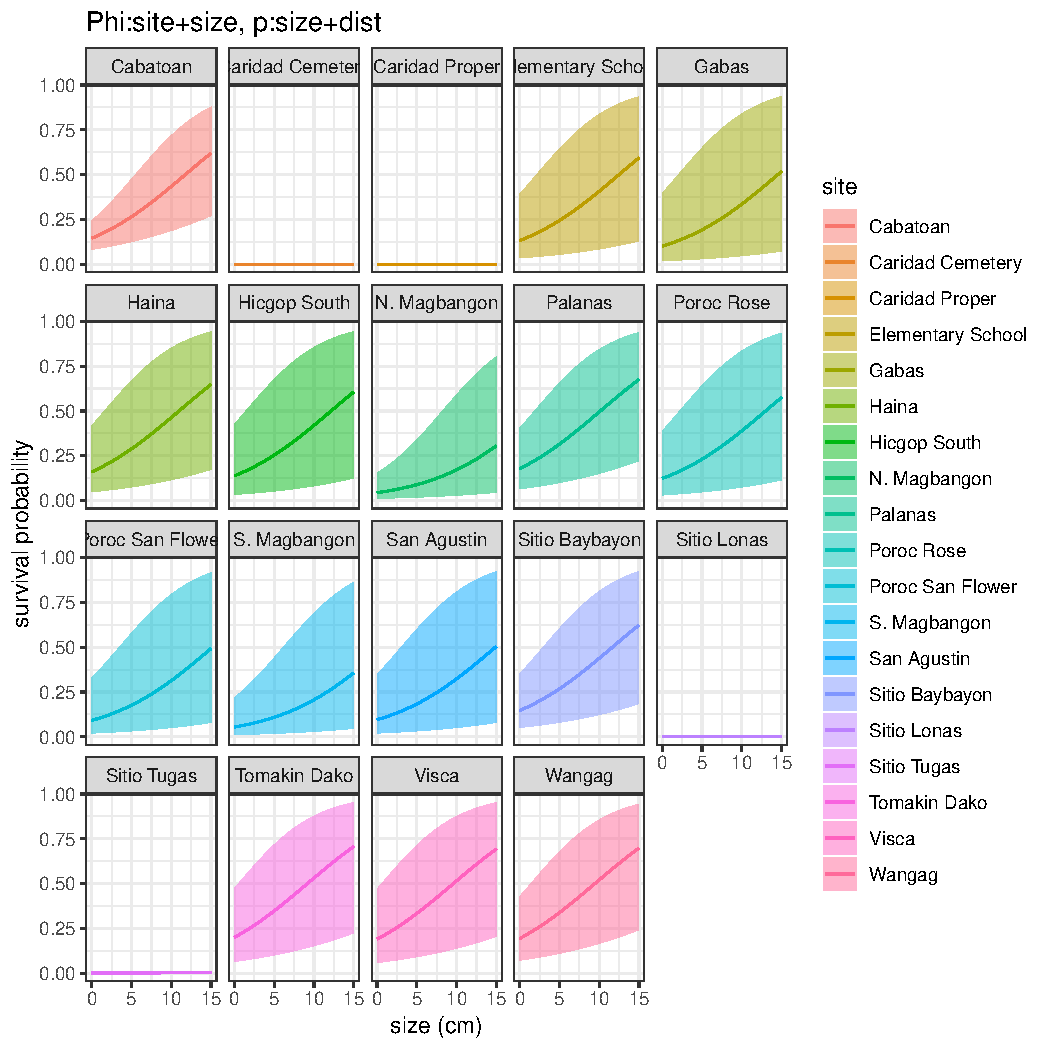
\includegraphics[width = 1.0\textwidth]{\detokenize{../Plots/FigureDrafts/APP_FIG_surv_by_size_and_site_Phisiteplussize_psizeplusdist.pdf}}
	\caption{Annual survival by size at each site. \label{APP_FIG_SurvBySizeAndSite}}
\end{figure}

% \paragraph{Recapture model} 
% The best model for log-odds recapture probability, accompanying the survival model in eqn.\ \ref{EQN_Survival}, has a size effect ($b_1 = -1.816 \pm 0.080$ SE, Fig.\ \ref{APP_FIG_RecapSizeDistEffect}a) and a negative effect of diver distance from the anemone ($b_2 = -0.171 \pm 0.021$ SE, Fig.\ \ref{APP_FIG_RecapSizeDistEffect}b), with intercept $b_{p_r} = 17.93 \pm 0.858$ SE:

% \begin{equation}
% \log(\frac{p_r}{1-p_r}) = b_{p_r} + b_1\text{size} + b_2d. \label{APP_EQN_MARK_Recapture}
% \end{equation}
% \begin{eqnarray}
% \log(\frac{\phi}{1-\phi}) &=& b_\phi + b_a\text{size} \\
% \log(\frac{p_r}{1-p_r}) &=& b_{p_r} + b_1\text{size} + b_2d. \label{EQN_Survival}
% \end{eqnarray}
%These results suggest that larger fish have higher annual survival, which is similar to survival estimates in other clownfish species (check Buston paper). 

% The negative effect of both size and distance suggest that divers are less likely to recapture larger fish and those at anemones far from areas sampled. %, with the chance of recapturing an average-sized fish falling below 5\% if a diver stays farther than XX from its home anemone.

% Add plot of distances to anems in different years?
% Add plot of effect of size and distance on recapture probability?
\begin{figure}[H] % 4 relationships among parameters
	\centering
	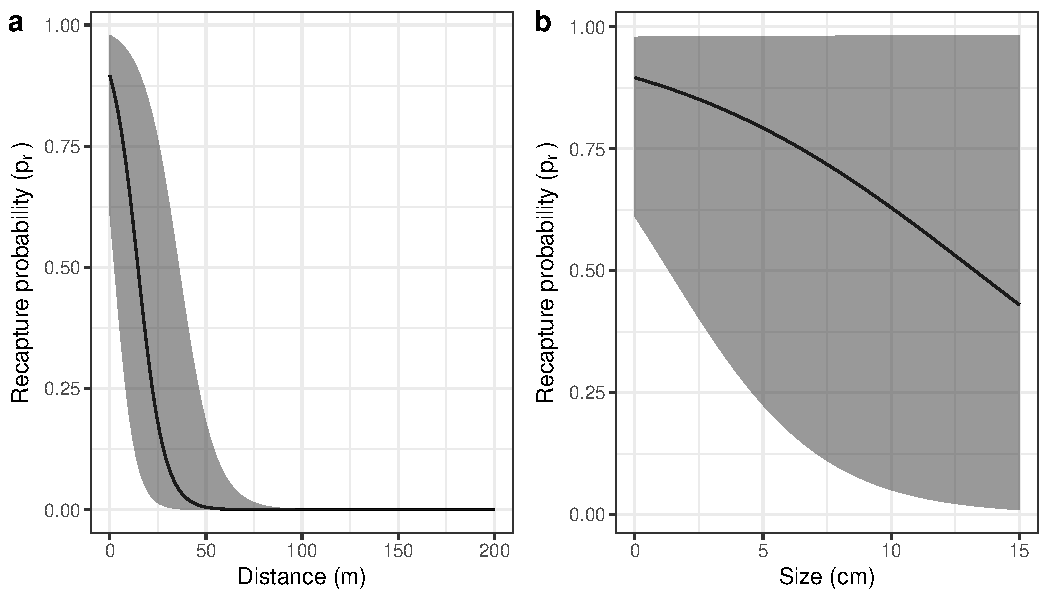
\includegraphics[width = 1.0\textwidth]{\detokenize{../Plots/FigureDrafts/APP_FIG_recap_effects_Phisiteplussize_psizeplusdist.pdf}}
	\caption{Effects of a) minimum distance between divers and the anemone where the fish was first caught and b) fish size on the probability the fish will be recaptured, estimated along with survival in a mark-recapture analysis. Size has a slightly negative effect on the probability of recapture - larger fish are stronger swimmers and more likely to flee the anemone when divers approach, but with high uncertainty at larger sizes. Distance also has a negative effect on recapture, as fish tend to stay close to their anemones and are not likely to be recaught if divers do not get close the their anemone. \label{APP_FIG_RecapSizeDistEffect}}
\end{figure}

% From the mark-recapture analysis of tagged and genotyped fish, we estimate mean values of $L_\infty = 10.71 \text{cm}$ (range of estimates 10.50 - 10.90 cm) and $K = 0.864$ (range of estimates 0.785 - 0.944) for the von Bertalanffy growth curve parameters (eqn.\ \ref{EQN_VBL}, Fig.\ \ref{FIG_ParameterInputs}b, Table \ref{APP_TAB_Params}). For juvenile and adult (post-recruitment) survival on a log-odds scale, the best-fit model has an effect of size, with coefficient $b_a = 0.169 \pm 0.028$ SE and intercept $b_\phi = -1.83 \pm 0.231$ SE (eqn.\ \ref{EQN_Survival}). The accompanying best-fit model for log-odds recapture probability has a negative size effect and a negative effect of diver distance from the anemone (eqn.\ \ref{APP_EQN_MARKRecapture}, Fig.\ \ref{APP_FIG_RecapSizeDistEffect}).

\newpage{}

\section{Result details and sensitivity}

\subsection{Abundance trends by site}

We use the number of females captured at each site in each sampling year, scaled by the proportion of habitat sampled at that site in that year and by the probability of capturing a fish, to estimate abundance trends for each site (Fig.\ \ref{APP_FIG_AbundanceBySite}).

\begin{figure}[H]  % Scaled estimates of females and trends by site
	\centering
	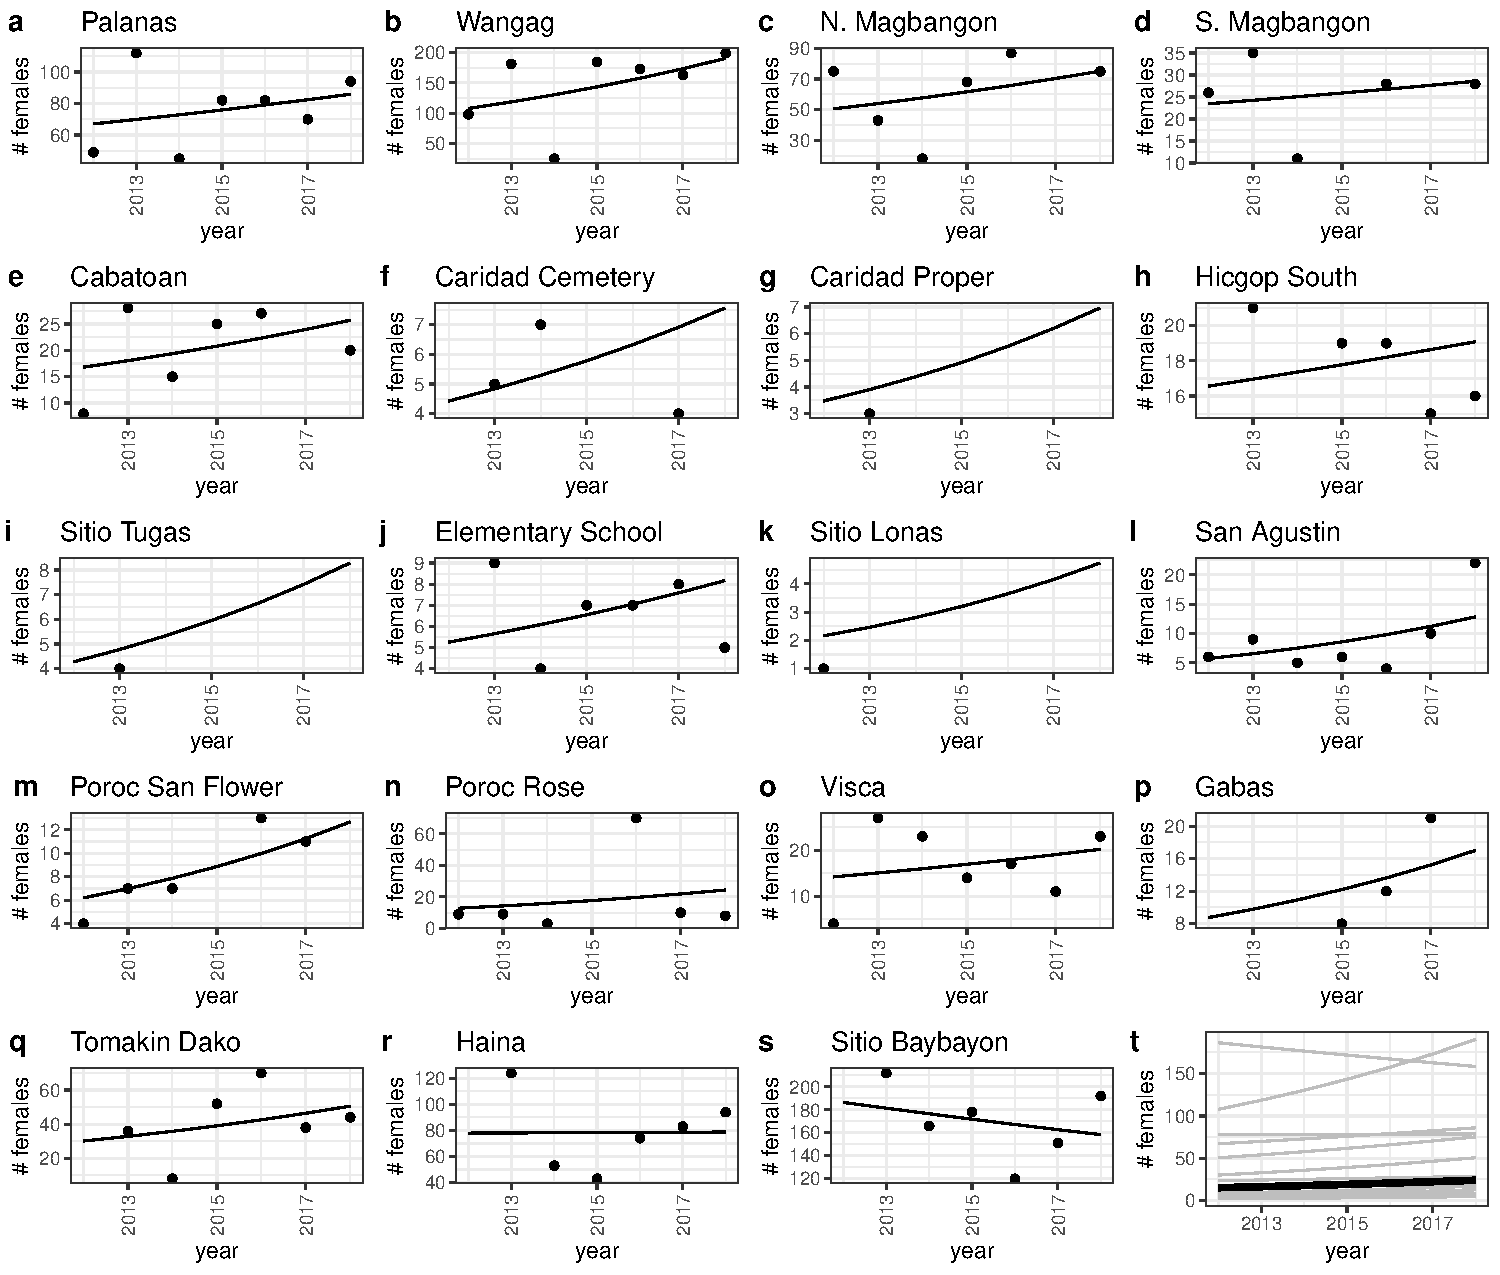
\includegraphics[width = 1.0\textwidth]{\detokenize{../Plots/FigureDrafts/Time_series_scaled_F_by_site_with_lines.pdf}}
	\caption{Scaled number of females captured (black dots) and abundance trends (black lines) by site from a mixed effects model with site as a random effect. \label{APP_FIG_AbundanceBySite}}
\end{figure}

\newpage{}

\subsection{Compensating for density dependence} \label{APP_SEC_noDD}
Estimating persistence metrics without compensating for density-dependence in our data gives us an understanding of whether individuals at our sites are able to replace themselves and whether our sites persist as in isolation at the current abundance levels, rather than at low abundance. Without compensation for early life density-dependence, all of our metrics show that the set of sites we sample is less likely to persist as an isolated network. We estimate egg-recruit survival ($S_e$) to be 7.8e-04 [1.2e-04, 0.033] and average lifetime recruit production ($\text{LRP}$) across sites to be 0.83 [0.28, 3.89], with XX\% of LRP estimates $\geq 1$. (Fig.\ \ref{APP_FIG_LRP_LocalReplacement_noDD}c). Our estimate of local replacement (LR), which estimates replacement for recruits from our sites returning to our sites implictly including dispersal, is 0.09 [0.03, 0.44]. 

When we calculate LR using all arriving recruits to our sites, however, rather than just those originating there, the best estimate is $> 1$ (1.22, with XX\% of values with uncertainty > 1), suggesting that there is recruit-recruit replacement at our sites when we include immigrant recruits.

We do not find any sites with a best estimate or uncertainty range of SP $>$ 1 (Figs.\ \ref{APP_FIG_SP_NP_realizedCmat_noDD}a), with the exception of the wide uncertainty bounds on SP for Caridad Cemetery. Our best estimate of the dominant eigenvalue of the realized connectivity matrix $\lambda_c$ is 0.21 [0.07, 0.92] with $p(\lambda \geq 1 = XX$ (Fig.\ \ref{APP_FIG_SP_NP_realizedCmat_noDD}c). 

\begin{figure}[H] % LRP and local replacement without DD compensation
	\centering
	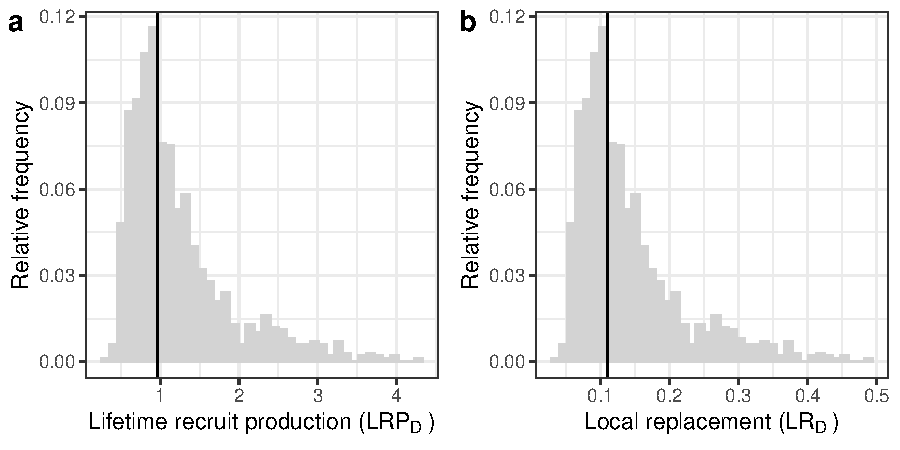
\includegraphics[width = 1.0\textwidth]{\detokenize{../Plots/FigureDrafts/APP_FIG_LRP_LocalReplacement_withoutDDconsidered_freq.pdf}}
	\caption{Estimates of a) LRP, and b) local replacement without compensating for density dependence in early life stages in our data, showing the best estimate (black solid line) and range of estimates considering uncertainty in the inputs. These estimates compare to those in \ref{FIG_Abun_LEP_LRP_LocalReplacement}c,d, where we correct for additional mortality in early life due to density dependence. \label{APP_FIG_LRP_LocalReplacement_noDD}}
\end{figure} 

\begin{figure}[H] % SP, realized connectivity matrix, NP without DD compensation
	\centering
	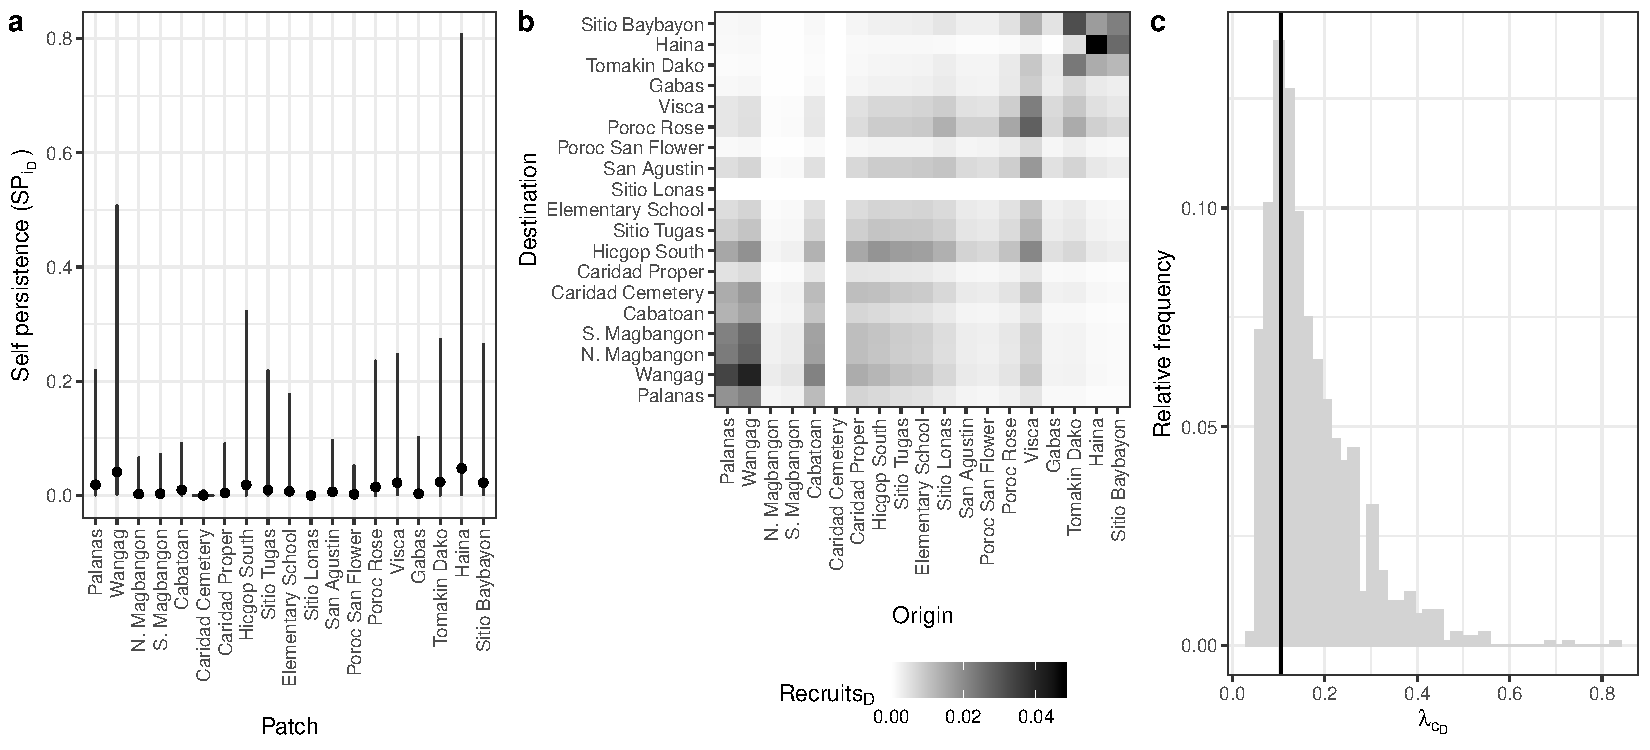
\includegraphics[width = 1.0\textwidth]{\detokenize{../Plots/FigureDrafts/APP_FIG_SP_NP_connMatrixR_withoutDDcompensation_freq.pdf}}
	\caption{Values of self-persistence (a), realized connectivity among sites (b), and network persistence (c) without compensation for density-dependence in early life stages in our data. For self-persistence (a) and network persistence (c), the best estimate is shown with in black (point for (a), line for (c)) and the range of estimates considering uncertainty is shown in grey. These estimates compare to those in \ref{FIG_SP_NP_realizedCmat} where we attempt to compesate for density dependence in early life stages. \label{APP_FIG_SP_NP_realizedCmat_noDD}}
\end{figure} 

\newpage{}

\subsection{LEP and LRP by site}

WRITE SOME TEXT!

\begin{figure}[H] % LEP by site
	\centering
	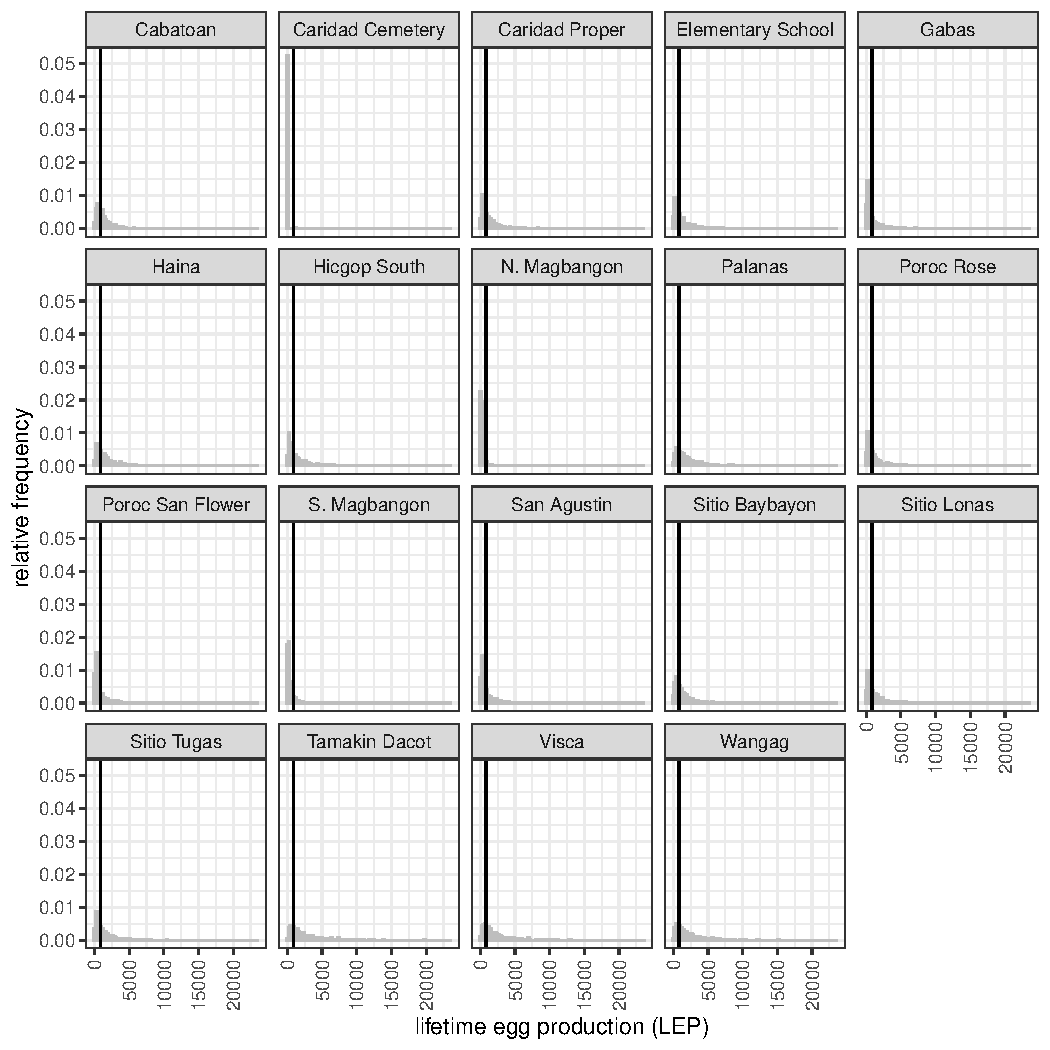
\includegraphics[width = 1.0\textwidth]{\detokenize{../Plots/FigureDrafts/APP_FIG_LEP_by_site.pdf}}
	\caption{Write a caption. \label{APP_FIG_LEP_by_site}}
\end{figure}

\begin{figure}[H] % LRP by site
	\centering
	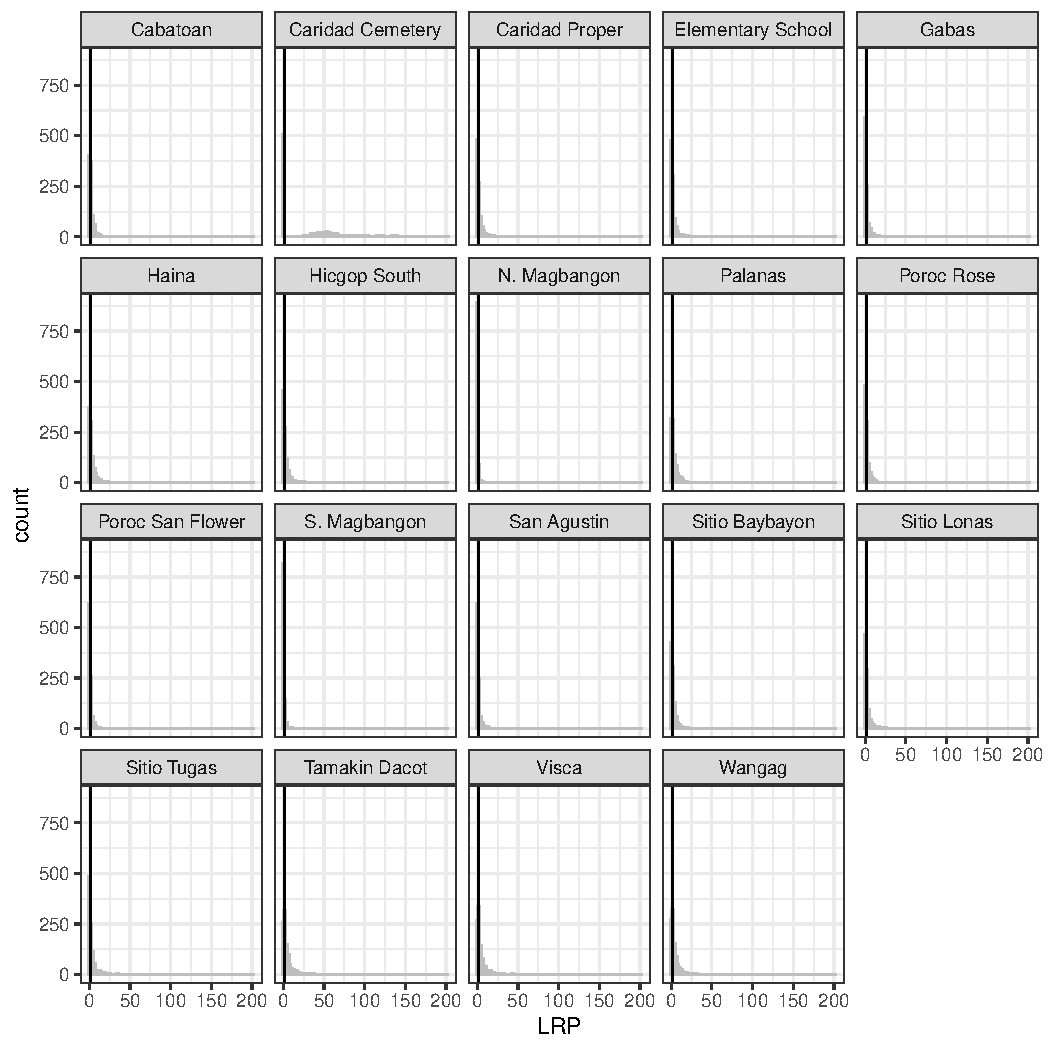
\includegraphics[width = 1.0\textwidth]{\detokenize{../Plots/FigureDrafts/APP_FIG_LRP_by_site.pdf}}
	\caption{Write a caption. \label{APP_FIG_LRP_by_site}}
\end{figure}

% \subsection{What-if analyses}

% To compare our replacement-based persistence results, which do not suggest that our sites make up a persistent metapopulation, with our abundance trends (Fig.\ \ref{FIG_FthroughTime}, which suggest that population abundances at our site have been relatively stable over our sampling period, we estimate recruits arriving at our sites per recruit there, regardless of the origin of the arriving recruits. We repeat our metric estimates but use all offspring genotyped at our sites, scaled by proportion habitat sampled within our sites $P_h$ and the probability of capturing a fish $P_c$, as our estimate of recruited tagged offspring. We find a value of $\text{LRP}_\text{local} = 1.22$ without compensating for density dependence and 2.06 if we do, both of which are $> 1$, suggesting our sites have persistent populations, though cannot necessarily persist alone, as our NP values are still $>1$.

% \paragraph{All genotyped offspring at our sites originated from our sites}

% \begin{figure}[H] % Do we see replacement if we consider all recruits when looking at recuits-per-recruit?
% 	\centering
% 	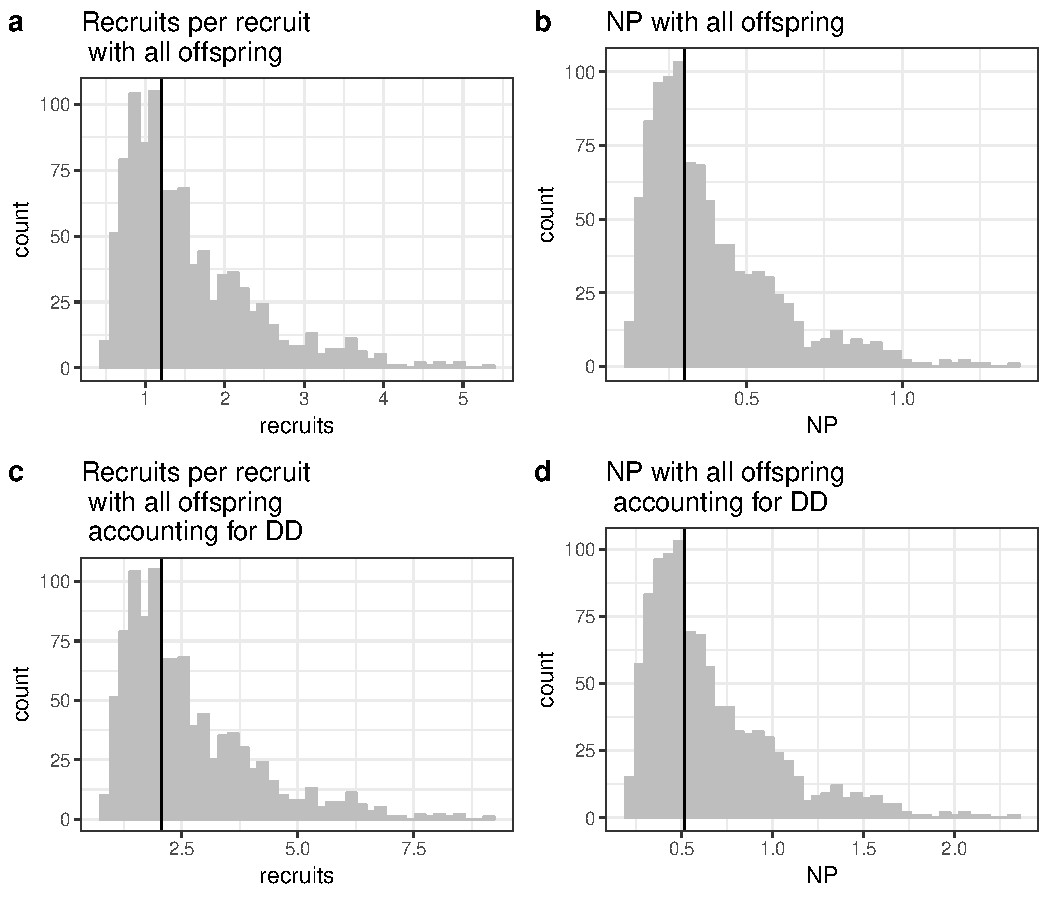
\includegraphics[width = 1.0\textwidth]{\detokenize{../Plots/PersistenceMetrics/Whatifs/LEP_R_and_NP_histograms_whatif_all_offspring.pdf}}
% 	\caption{a) Recruits per recruit when we consider all arriving recruits to have originated from our sites. b) Range of values of NP considering all arriving recruits to be offspring from our sites, with the best estimate in a black solid line. \label{APP_FIG_AllOffspringWhatIf}}
% \end{figure}

\subsection{Sensitivity to parameters}

The range of parameters not shown in the main text (Fig.\ \ref{FIG_ParameterInputs}):

\begin{figure}[H] % Range of parameter inputs for uncertainty runs
	\centering
	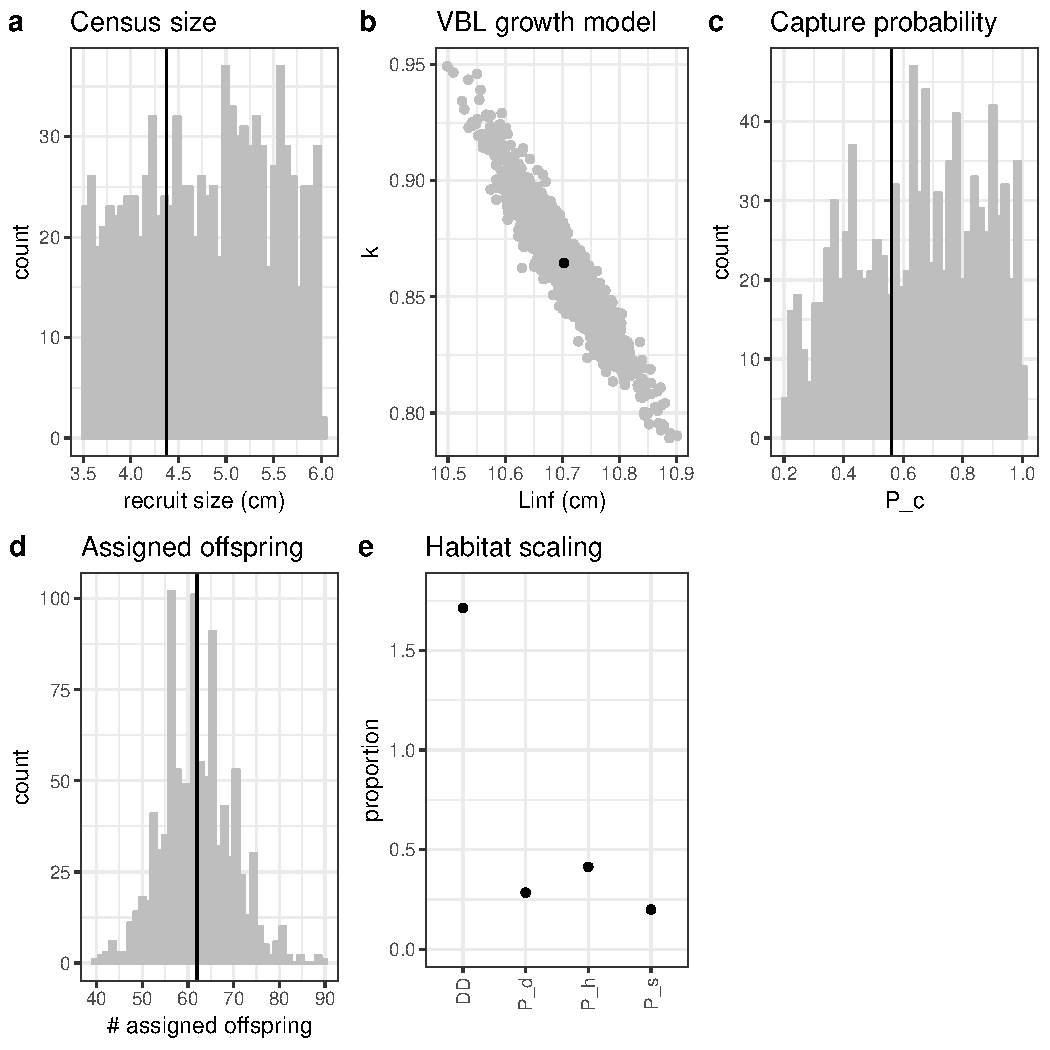
\includegraphics[width = 1.0\textwidth]{\detokenize{../Plots/FigureDrafts/APP_FIG_Parameter_inputs.pdf}}
	\caption{Range of parameter inputs for uncertainty runs with all uncertainty included, where the black line or point is the value used for the best estimate: a) $\text{size}_\text{recruit}$, the census size at which fish are considered to have recruited after egg-recruit survival occurs; b) the parameters $L\infty$ and $K$ of the von Bertalanffy growth model; c) $P_c$, the probability of capturing a fish; d) number of offspring assigned back to parents in the parentage analysis; e) factors that scale the number of estimated recruits from our site based on density-dependence in settler success (DD), proportion of the dispersal kernel captured by our sampling region ($P_d$), the cumulative proportion of our sites we sampled over time ($P_h$), and the proportion of our sampling area that is habitat ($P_s$). \label{APP_FIG_UncertaintyInputs}}
\end{figure}

% Range of parameters used as input for uncertainty runs

% \begin{figure}[H] % Range of parameter inputs for uncertainty runs
% 	\centering
% 	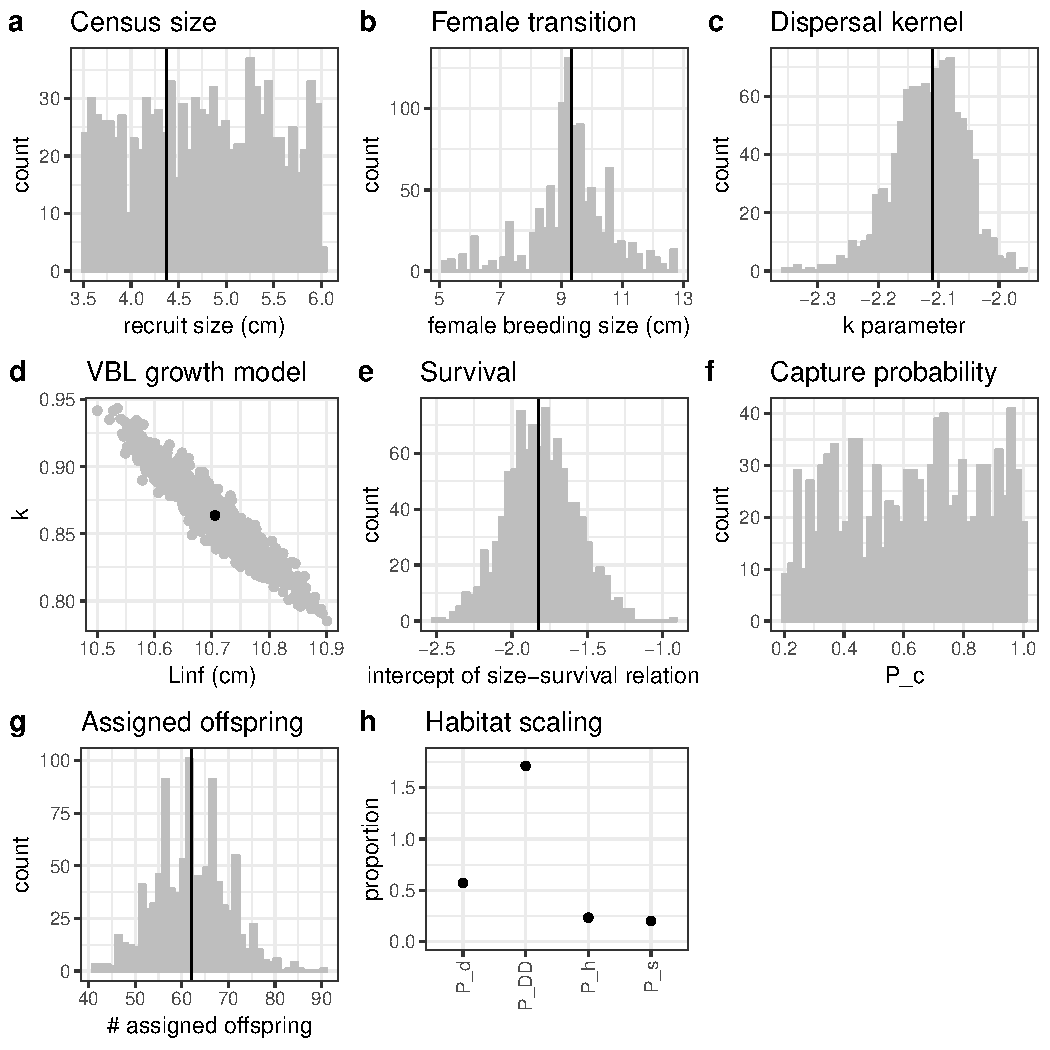
\includegraphics[width = 1.0\textwidth]{\detokenize{../Plots/FigureDrafts/Uncertainty_inputs.pdf}}
% 	\caption{Range of parameter inputs for uncertainty runs with all uncertainty included: a) $\text{size}_\text{recruit}$, the census size at which fish are considered to have recruited after egg-recruit survival occurs; b) $L_f$, the size at which fish transition from male to female and their reproductive output is included in the estimate of lifetime egg production (LEP); c) $k_d$, the scale parameter in the dispersal kernel; d) the parameters $L\infty$ and $K$ of the von Bertalanffy growth model; e) the intercept $b_\phi$ of the adult size-dependent survival relationship; f) $P_c$, the probability of capturing a fish; g) number of offspring assigned back to parents in the parentage analysis; h) factors that scale the number of estimated recruits from our site based on density-dependence in settler success (DD), proportion of the dispersal kernel captured by our sampling region ($P_d$), the cumulative proportion of our sites we sampled over time ($P_h$), and the proportion of our sampling area that is habitat ($P_s$). \label{APP_FIG_UncertaintyInputs}}
% \end{figure}

% % Relationships among parameters - MAKE A NEW ONE OF THESE???

% \begin{figure}[H] % 4 relationships among parameters
% 	\centering
% 	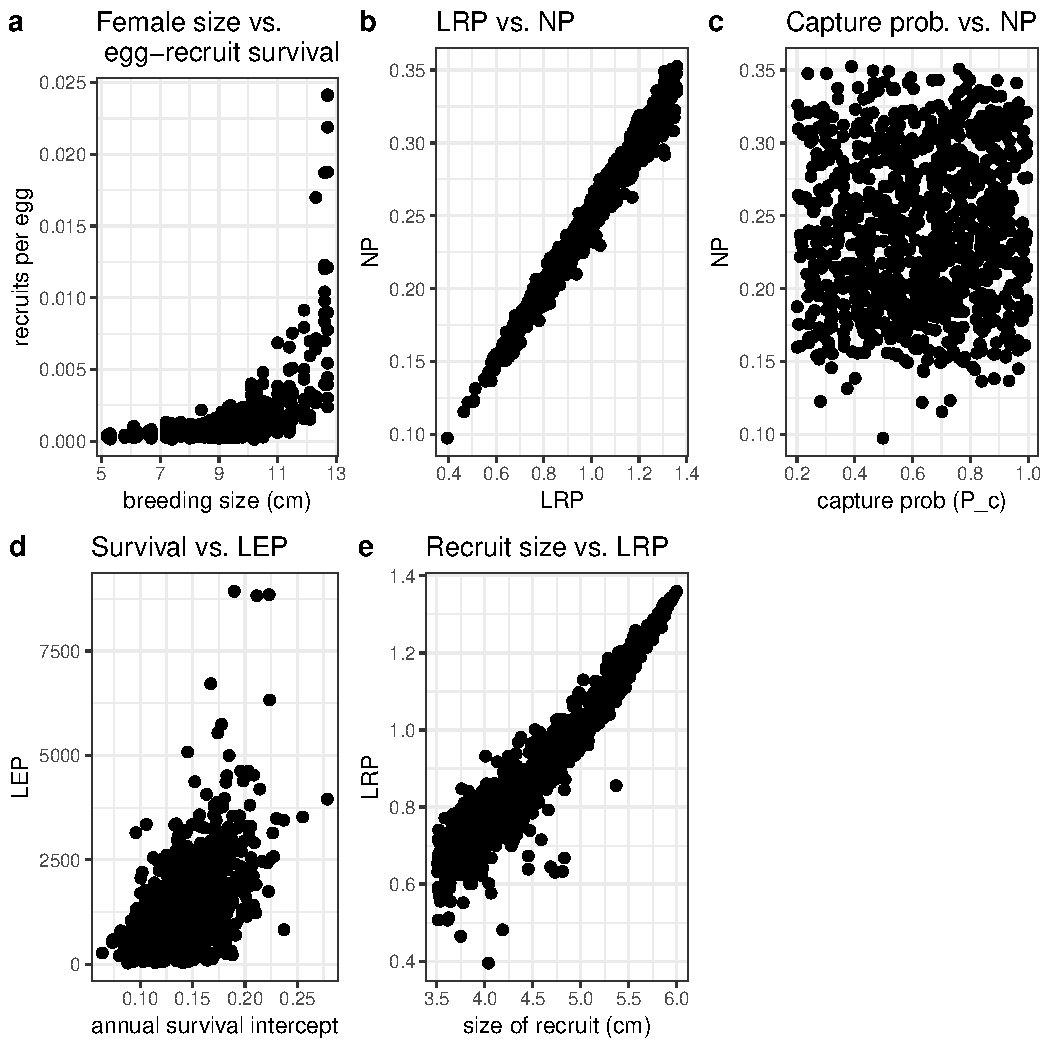
\includegraphics[width = 1.0\textwidth]{\detokenize{../Plots/FigureDrafts/Param_metric_relationships.pdf}}
% 	\caption{Relationships among parameters and metrics. a) We only count reproductive effort by fish in the female stage so the higher the transition size to breeding female, the fewer eggs parents are considered to produce, which increases the estiamted egg-recruit survival. b) LRP strongly affects NP by changing the number of potential recruits dispered through the connectivity matrix. c) The probability of capturing a fish does not have a clear relationship to NP. d) LEP is higher with higher survival estimates because fish are more likely to survive longer as reproducing adults. e) The size we consider to be a recruit marks the transition of mortality included in egg-recruit survival to mortality being captured by annual adult survival. Because we do not have the data to change egg-recruit survival to account for different recruit sizes, increasing the recruit size increases LRP by wrapping more mortality into the egg-recruit survival estimate, rather than LEP. \label{APP_FIG_ParamMetricRelationships}}
% \end{figure} % Think about a better way to explain (e) and whether we should even include it.

\subsection{Effects of different types of uncertainty on metrics}

% WRITE AN OVERALL SUMMARY, REFERENCE FIGS BELOW! (all have DD included)

%\paragraph{Effects of different types of uncertainty on LEP)}

% WRITE A SUMMARY!!
% Annual survival post-recruitment provides drives most of the uncertainty in LEP, as lower survivals keep fish from reaching and staying at large breeding sizes, with higher fecundity. The transition size to breeding female also drives uncertainty in LEP - the higher the transition size to female, the less time the fish has at a size where its reproduction is counted in LEP. 

\begin{figure}[H] % Uncertainty in LEP
	\centering
	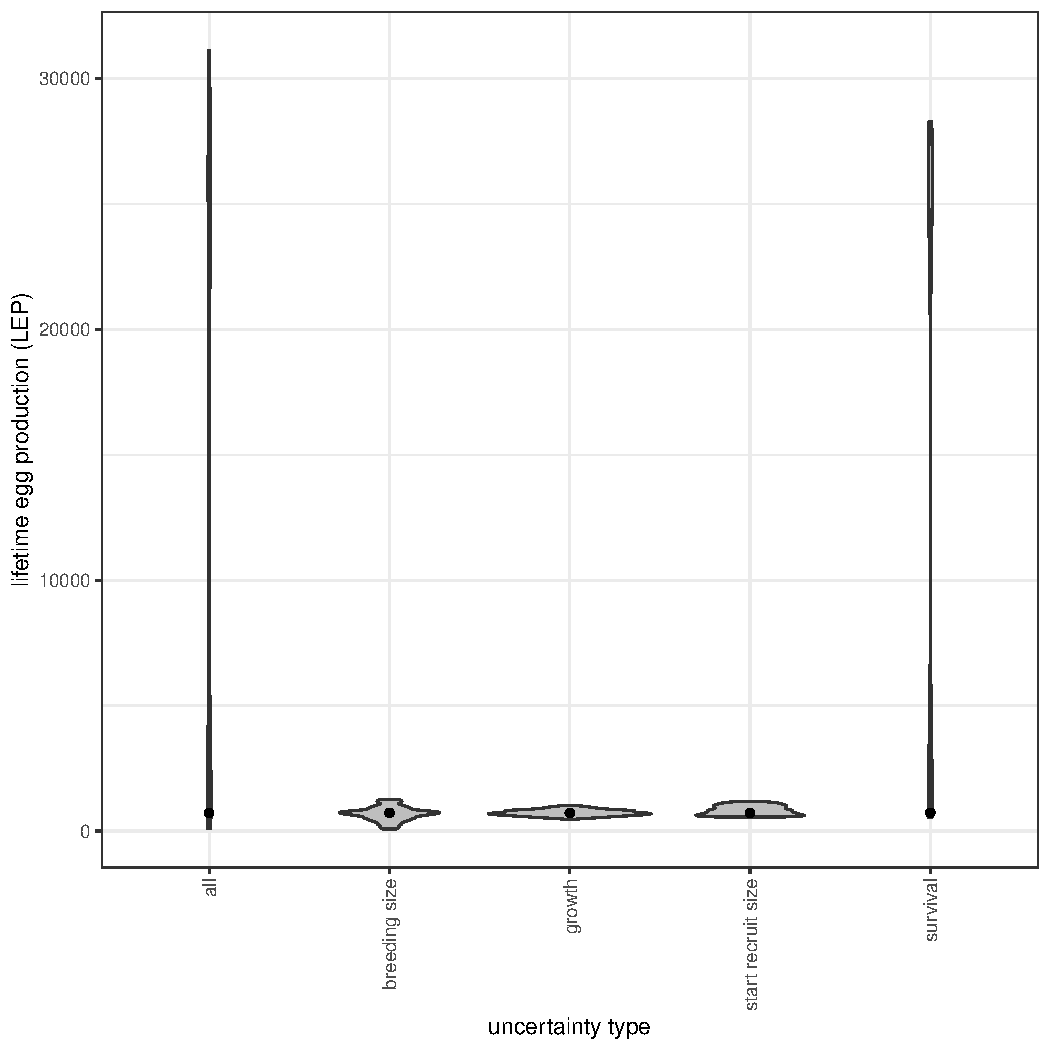
\includegraphics[width = 1.0\textwidth]{\detokenize{../Plots/FigureDrafts/LEP_uncertainty_by_param.pdf}}
	\caption{The contribution of different sources of uncertainty in LEP. \label{APP_FIG_Uncertainty_LEP}}
\end{figure}

%\paragraph{Effects of different types of uncertainty on LRP}

%WRITE A SUMMARY!
% Most of the uncertainty in LRP comes from uncertainty in the size of a recruit. This is an artifact of our sampling, where we are unable to estimate egg-recruit survival differently to account for changes in the size of a recruit, so raising the size of a recruit reduces the mortality included in LRP without increasing the mortality included in egg-recruit survival, as it should in an ideal situation.

\begin{figure}[H] % Uncertainty in LEP_R 
	\centering
	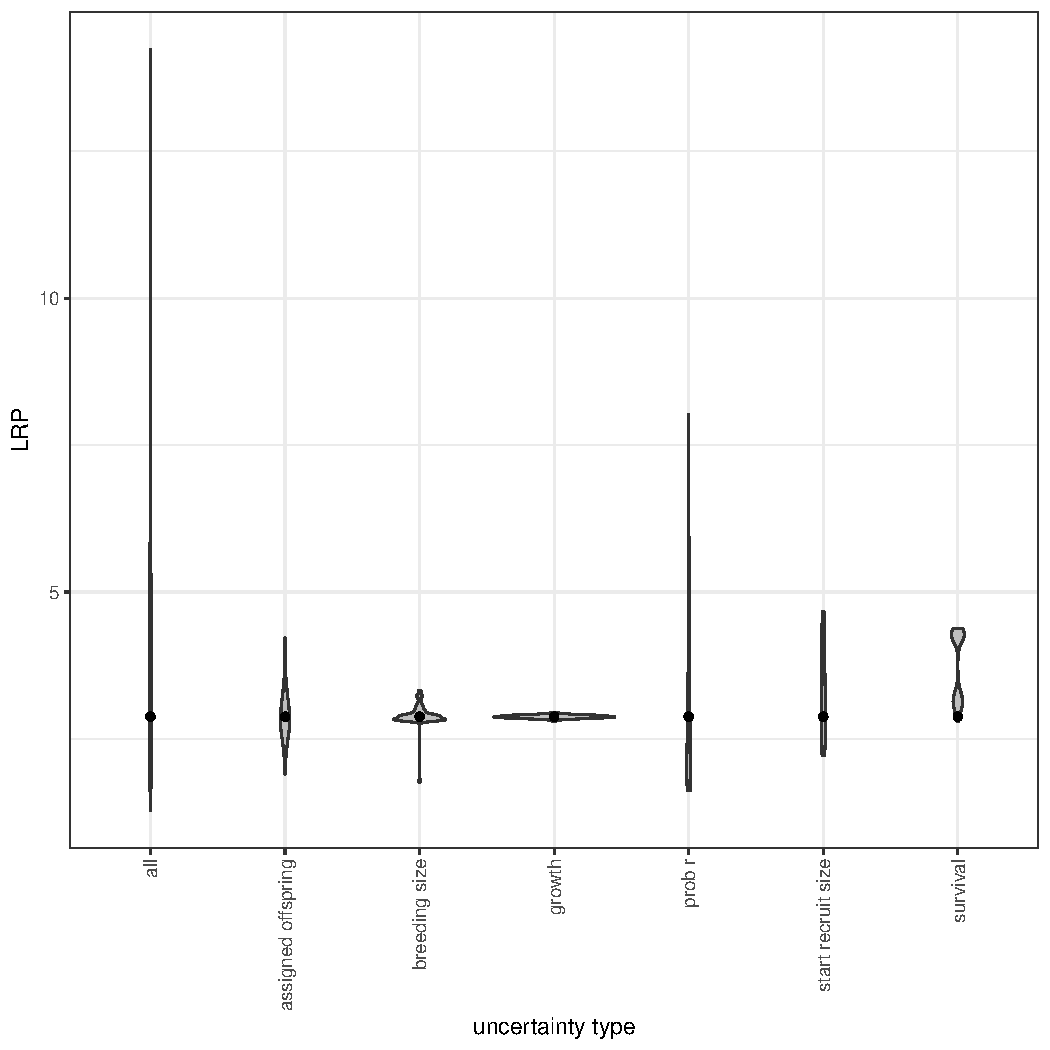
\includegraphics[width = 1.0\textwidth]{\detokenize{../Plots/FigureDrafts/LRP_uncertainty_by_param.pdf}}
	\caption{The contribution of different sources of uncertainty in LRP. \label{APP_FIG_Uncertainty_LEP_R}}
\end{figure}

% old note: check plots, weird that assigned offspring and prob_r are just points (unless I don't understand how violins work? Shouldn't they be essentially horizonal lines if all runs have the same value, kind of like growth? Also, why does breeding size have such a different shape for LRP and LEP? Seems weird...
% \begin{figure}[H] % Uncertainty in LEP_R with DD accounted for
% 	\centering
% 	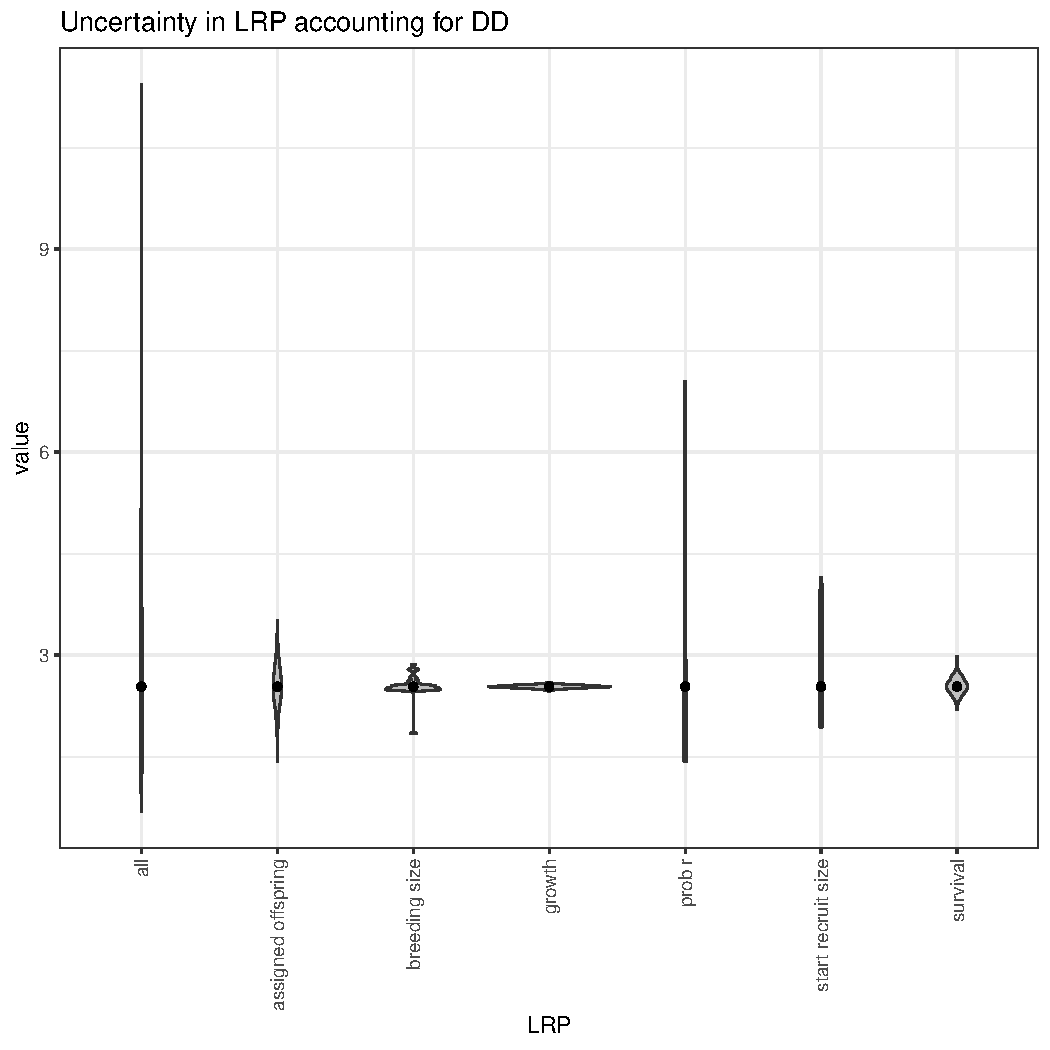
\includegraphics[width = 1.0\textwidth]{\detokenize{../Plots/FigureDrafts/LEP_R_uncertainty_breakdown_with_DD.pdf}}
% 	\caption{The contribution of different sources of uncertainty in LRP, when we account for density-dependence in egg-recruit survival. \label{APP_FIG_Uncertainty_LEP_R_DD}}
% \end{figure}

%\paragraph{Egg-recruit survival ($S_e$)}

% WRITE A SUMMARY!! 
\begin{figure}[H] % Uncertainty in recruits-per-egg
	\centering
	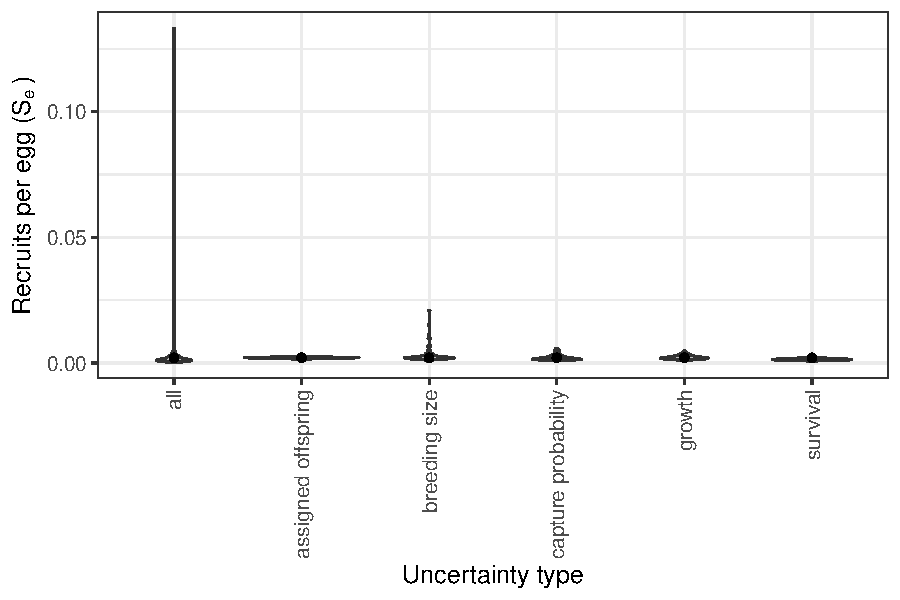
\includegraphics[width = 1.0\textwidth]{\detokenize{../Plots/FigureDrafts/RperE_uncertainty_by_param.pdf}}
	\caption{The contribution of different sources of uncertainty in egg-recruit survival. \label{APP_FIG_Uncertainty_RperE}}
\end{figure}

% \begin{figure}[H] % Uncertainty in recruits-per-egg with DD accounted for
% 	\centering
% 	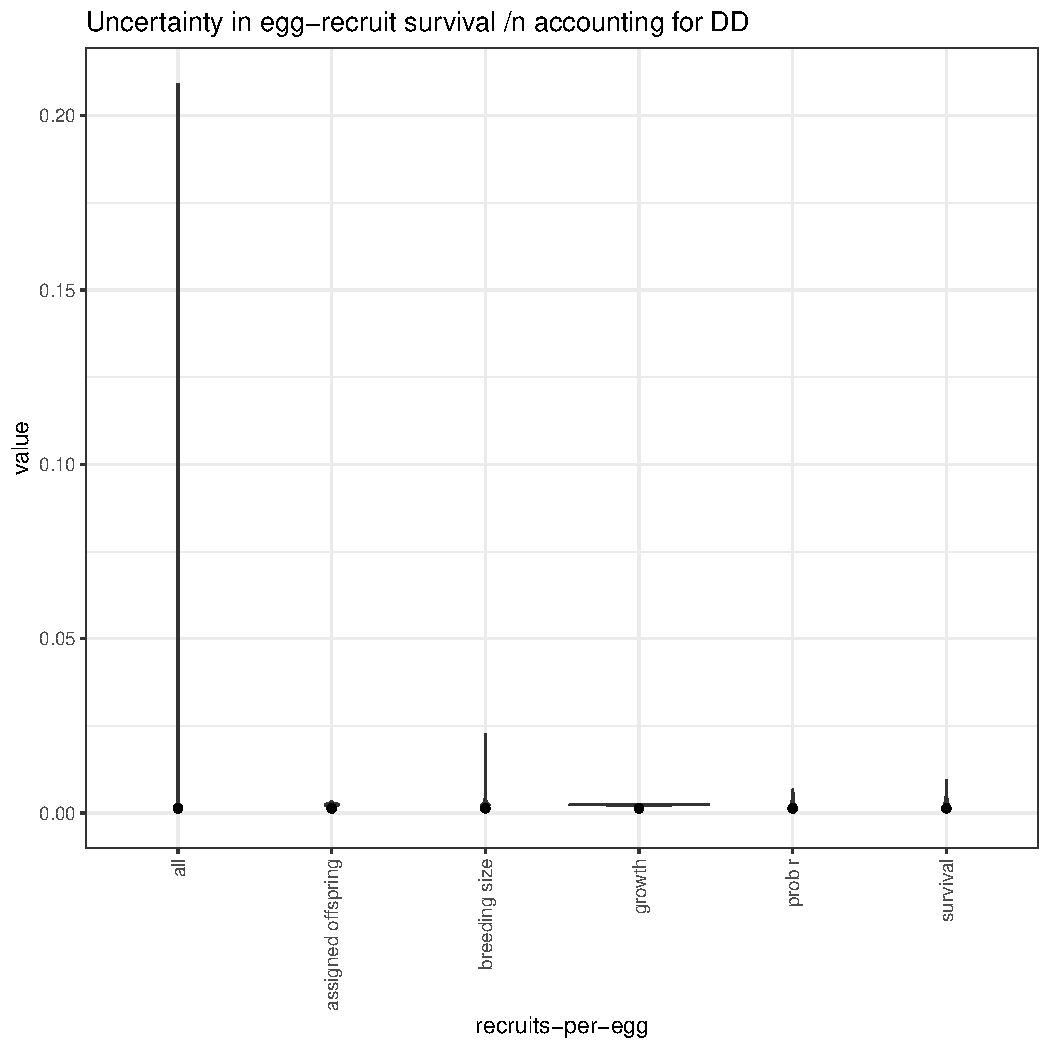
\includegraphics[width = 1.0\textwidth]{\detokenize{../Plots/FigureDrafts/RperE_uncertainty_breakdown_DD.pdf}}
% 	\caption{The contribution of different sources of uncertainty in egg-recruit survival when we account for density-dependence in egg-recruit survival. \label{APP_FIG_Uncertainty_RperE_DD}}
% \end{figure}

%\paragraph{Network persistence (NP)}

% WRITE A SUMMARY!
\begin{figure}[H] % Uncertainty in NP
	\centering
	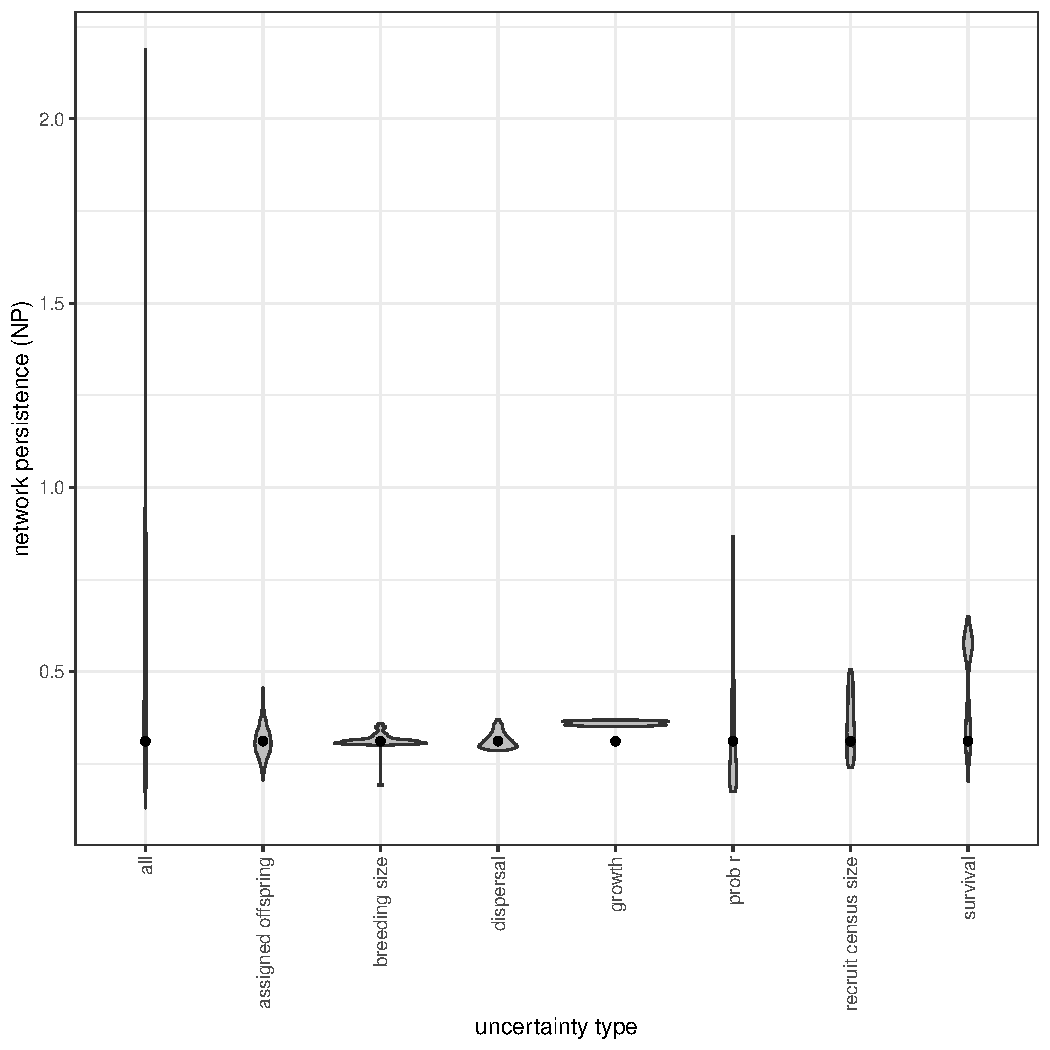
\includegraphics[width = 1.0\textwidth]{\detokenize{../Plots/FigureDrafts/NP_uncertainty_by_param.pdf}}
	\caption{The contribution of different sources of uncertainty in NP. \label{APP_FIG_Uncertainty_NP}}
\end{figure}

% \begin{figure}[H] % Uncertainty in NP with DD accounted for
% 	\centering
% 	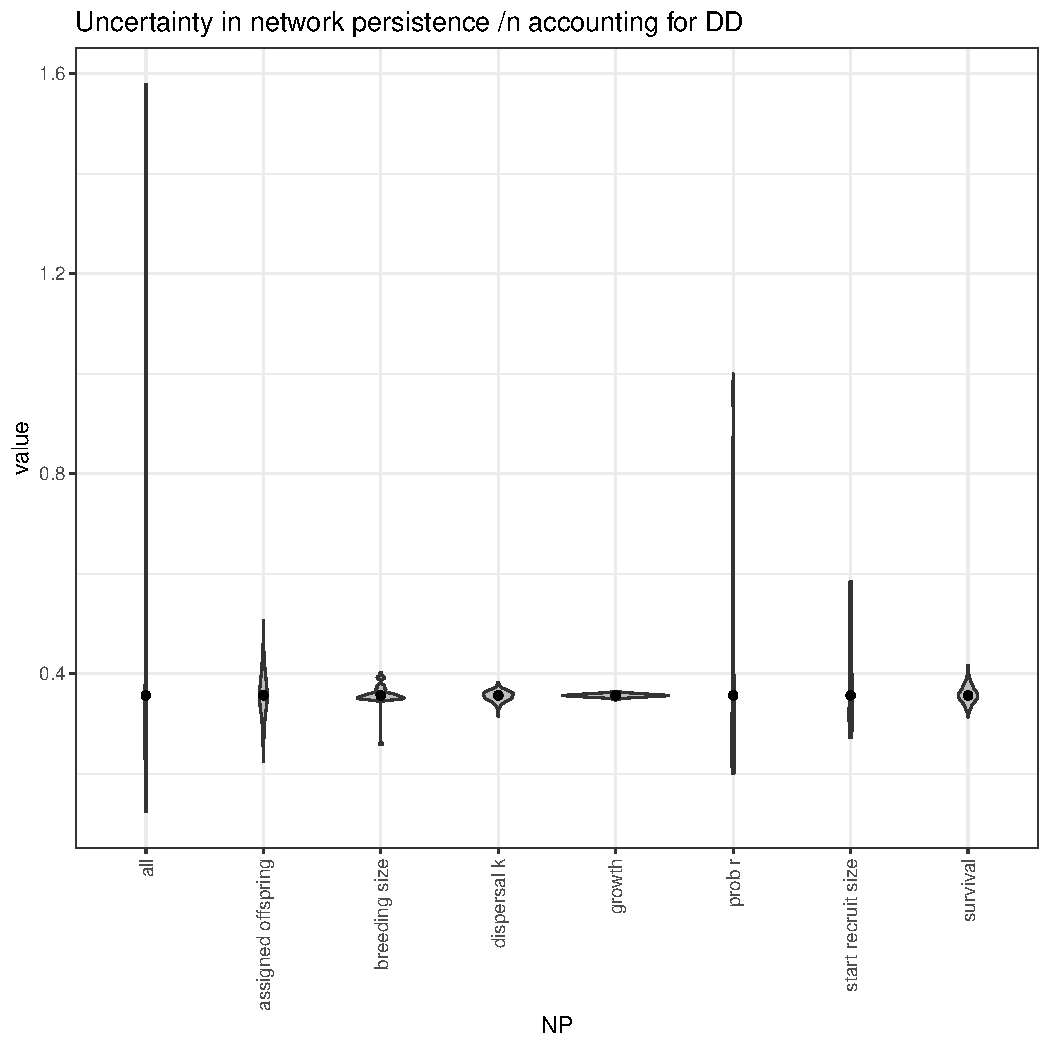
\includegraphics[width = 1.0\textwidth]{\detokenize{../Plots/FigureDrafts/NP_uncertainty_breakdown_DD.pdf}}
% 	\caption{The contribution of different sources of uncertainty in NP when we account for density-dependence in egg-recruit survival. \label{APP_FIG_Uncertainty_NP_DD}}
% \end{figure}

\newpage{}

%\bibliography{../../../BibTexReferences}
\bibliography{BibTexReferences}
\bibliographystyle{plainnat}

% NEED TO ADD IAN IMAGES REFERENCES
% SCUBA diver in scaling up recruits figure: \url{https://ian.umces.edu/imagelibrary/displayimage-5410.html}, downloaded 11/22/19
\end{document}